\documentclass[11pt, a4paper,oneside]{book}

\usepackage{caption}
\usepackage{a4wide}
\usepackage{makeidx}
\usepackage{float}
\usepackage{listings}
\usepackage{color}
\usepackage{textcomp}
\usepackage{alltt}
\usepackage{amsmath}
\usepackage{times}
\usepackage{ifpdf}
\usepackage{graphicx}
\usepackage{color} %colors in text
\usepackage{textcomp} % 
\usepackage[T1]{pbsi} %hand writting nice 
\usepackage[T1]{fontenc} %more fonts
\usepackage{mathrsfs} % letters for math
\usepackage{amsmath} % math formulas
\usepackage[all]{xy} % for drawing
\usepackage{listings}
\usepackage{amssymb}
%\usepackage[parfill]{parskip}
\definecolor{gray}{rgb}{0.7,0.7,0.7} 
\usepackage{enumerate} %for enumerate
\usepackage{subfigure}
\usepackage{epsfig}
\usepackage{float}
\usepackage{algorithm}
\usepackage[noend]{algorithmic}
\usepackage[dvipdfm]{hyperref}
\usepackage{multicol}
\usepackage{sectsty}
\usepackage{multirow}
%\ifpdf
%\usepackage[pdftex,
%            pagebackref=true,
%            colorlinks=true,
%            linkcolor=blue,
%            unicode
%           ]{hyperref}
%\else
%\usepackage[ps2pdf,
%            pagebackref=true,
%            colorlinks=true,
%            linkcolor=blue,
%            unicode
%           ]{hyperref}
%\usepackage{pspicture}
%\fi
\usepackage[utf8]{inputenc}
\makeindex
\setcounter{tocdepth}{3}
%\usepackage[light,condensed,math]{kurier}
%\renewcommand{\thechapter}{\Roman{chapter}}
%DEFINE NEW COMMANDS_________________________________________________________
%\newcommand{\clearemptydoublepage}{%
%  \newpage{\pagestyle{empty}\cleardoublepage}%
%}
\newcommand{\ds}{\displaystyle}
\newcommand{\todo}[1]{\textcolor{red}{\textbf{#1}}}
\newcommand{\fade}[1]{\textcolor{gray}{\textbf{#1}}}
\newcommand{\myemph}[1]{{\normalfont\emph{#1}}}
\newcommand{\tit}{\textit}

\usepackage[left=4cm, right=4cm, top=4cm, bottom=3.9cm]{geometry}
%____________________________________________________________________________
\begin{document}
	%THE TITLE PAGE & STUFF_________________________________________________________________
	%\fontfamily{arial}\selectfont
	%\fontfamily{courier-ttf}\selectfont
	%\fontfamily{comicsans}\selectfont
	%\fontfamily{franklingothic}\selectfont
	%\fontfamily{impact}\selectfont Impact
	%\fontfamily{palatino-ttf}\selectfont
	%\fontfamily{sylfaen}\selectfont 
	%\fontfamily{tahoma}\selectfont
	%\fontfamily{times-ttf}\selectfont 
	%\fontfamily{trebuchet}\selectfont 
	%\fontfamily{verdana}\selectfont 
	\fontfamily{georgia}\selectfont\normalsize

	\hypersetup{pageanchor=false}
	\begin{titlepage}
	\begin{figure}[!hbtp]
		\begin{flushright}
			
\epsfig{file=images/uva.eps, width=0.3\linewidth}
		\end{flushright}
	\end{figure}
	\vspace*{2cm}
	\begin{center}
	\rule{\linewidth}{1px}\\[10pt]
	\Huge{Texture Synthesis for Material Classification}
	\rule{\linewidth}{1px}\\[10pt]
	\vspace*{1cm}
	\large{Master\rq s Thesis in Artificial Intelligence -- Intelligent Systems}
	\large
	\vspace*{4cm}
	\begin{multicols}{2}
		\begin{flushleft}
			{\emph{Author:}\\
			Jasper van Turnhout\\
			\textit{jturnhou@science.uva.nl}\\ 
			Student number: 0312649}  
		\end{flushleft}
		\begin{flushleft}
			{\emph{Supervisors:}\\
			\href{mailto:Th.Gevers@uva.nl}{Prof. dr. Theo Gevers}\\
			\href{mailto:geusebroekuva.nl}{Dr. Jan-Mark Geusebroek}\\
			Informatics Institute, Faculty of Science, University of Amsterdam\\
			}
		\end{flushleft}
	\end{multicols}
	\end{center}
	\vspace*{6cm}
	\end{titlepage}
	%ABSTRACT PAGE____________________________________________________________________________
	\thispagestyle{empty}
	\section*{Abstract}
		Research description comes here
	%CONTENT PAGE____________________________________________________________________________
	\newpage
	\pagenumbering{roman}
	\tableofcontents
	%CHAPTERS & SUB-CHAPTERS____________________________________________________________________
	\newpage
	\pagenumbering{arabic}
	\hypersetup{pageanchor=true}
	\chapter{Introduction}
	\hypertarget{Introduction}{
}

For human perception, recognizing materials is a very important aspect in our visual system. We can do this flawlessly for a great number of different materials. As a human, we can easily determine whether a surface is smooth, rough, soft or hard by just looking at it. We are also capable of recognizing  materials under great variety of visual conditions. For example, when observing a car from an arbitrary point of view, we always perceive the surface of the car differently when considering the light reflected on the metallic surface which differs from viewpoint to viewpoint. Yet, we have no problem in classifying this surface as metal. The same accounts for many other materials we perceive on a daily base.

Material recognition is a field of research in computer vision with the goal to develop classification systems that can identify various material categories observed in daily life. Examples of such categories are metal, wood, fabric, plastic and glass. Material recognition differs and should not be confused with object recognition and texture recognition. This difference is illustrated in figure \ref{fig:ObjectRecognition} and \ref{fig:TextureRecognition}. A system capable of recognizing materials can greatly enhance the performance of object recognition or scene recognition.

Research has been done on several different material databases and good recognition accuracies have been reported. However, there are suggestions that the accuracies reported are all database dependent \cite{ExploringFeatures} since none of these databases could possibly capture the large variation in appearance of material classes. The large variation of a material class is also addressed as the intra-class variation. 

In this research, we investigate how realistic image synthesis can be employed to create synthetic image data for various material classes. With the aid of image synthesis it is possible to generate infinite amounts of data with arbitrary viewpoint and illumination conditions. This makes it possible to create image data that is not present in material databases, thus making it possible to increase the intra-class variation of material classes.

This chapter gives a short introduction to the problem of material recognition and how image synthesis can be applied to improve recognition performance.

\begin{figure}[htbp!]
	\begin{center}
		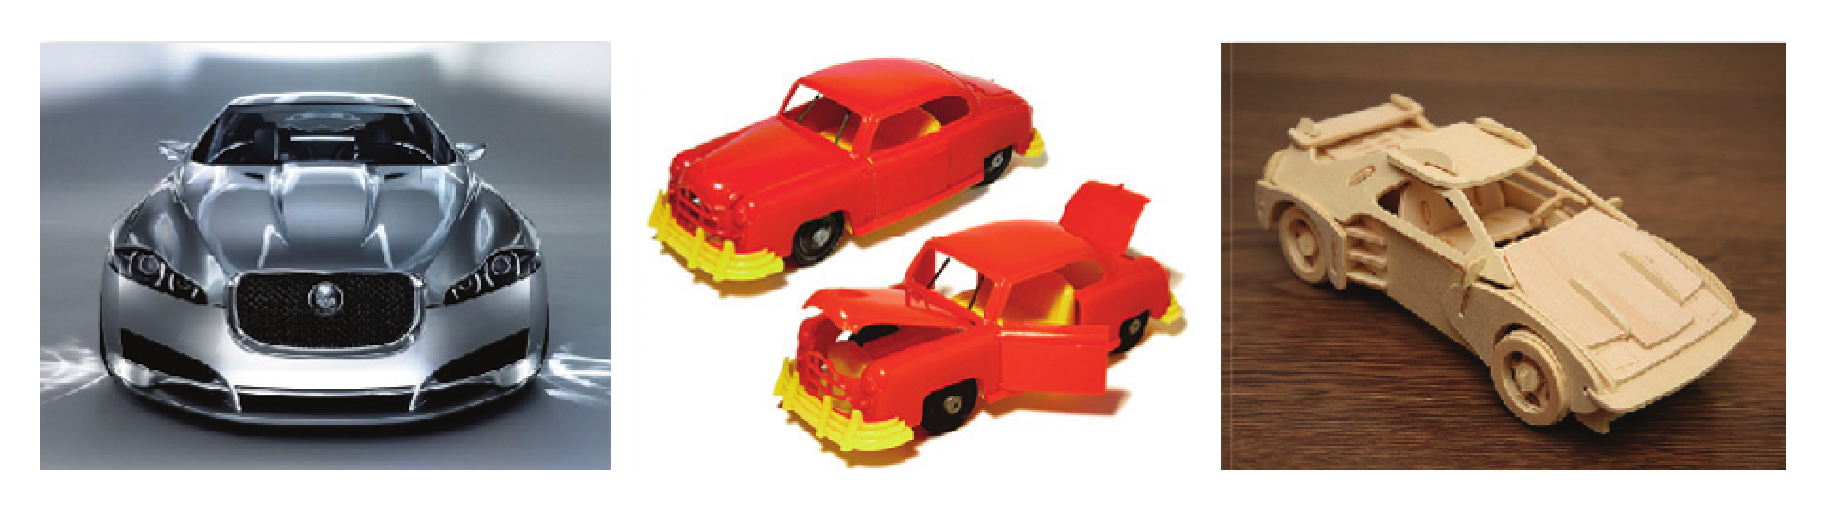
\epsfig{file=images/ObjectRecognition.eps, width=0.6\linewidth}
	\end{center}
	\caption{{\it Object recognition and material recognition: all three pictures depict the same object. However, they are made from metal, plastic and wood respectively. Image adapted from \cite{ExploringFeatures}.}}
	\label{fig:ObjectRecognition}
\end{figure}

\begin{figure}[htbp!]
	\begin{center}
		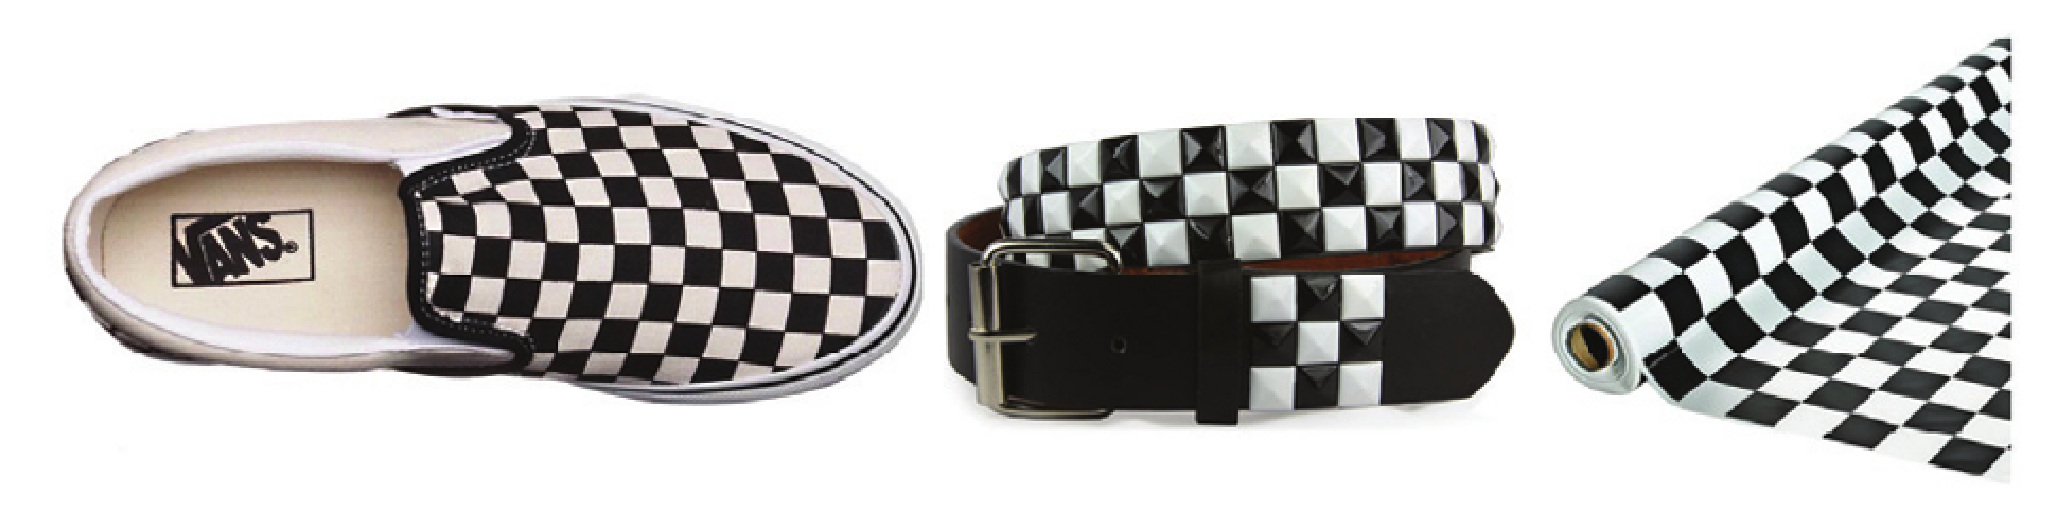
\epsfig{file=images/TextureRecognition.eps, width=0.6\linewidth}
	\end{center}
	\caption{{\it Texture recognition and material recognition: all three pictures depict the same pattern. However, they are made from fabric, plastic and paper respectively. Image adapted from \cite{ExploringFeatures}.}}
	\label{fig:TextureRecognition}
\end{figure}

\section{Material Recognition}
Material recognition is defined as the task to correctly classify a novel image from a material surface. When building a system for material recognition, prediction of a material class is done preferably on a single image of a material surface. This creates a difficult task as the variation in appearances of materials is considerably enhanced by illumination differences or arbitrary viewpoints. Some examples of how much a surface can vary are shown in figure \ref{fig:PhoTexExamples}.

In recent research, material databases have been created containing various illumination and viewpoint conditions that try to capture the large variety within each  material class. The difficulty is to obtain robust features from the image data that covers various occurrences of materials with different spatial properties as well as distinct illumination properties. 

\begin{figure}[htbp!]
	\begin{center}
		\subfigure[aab]{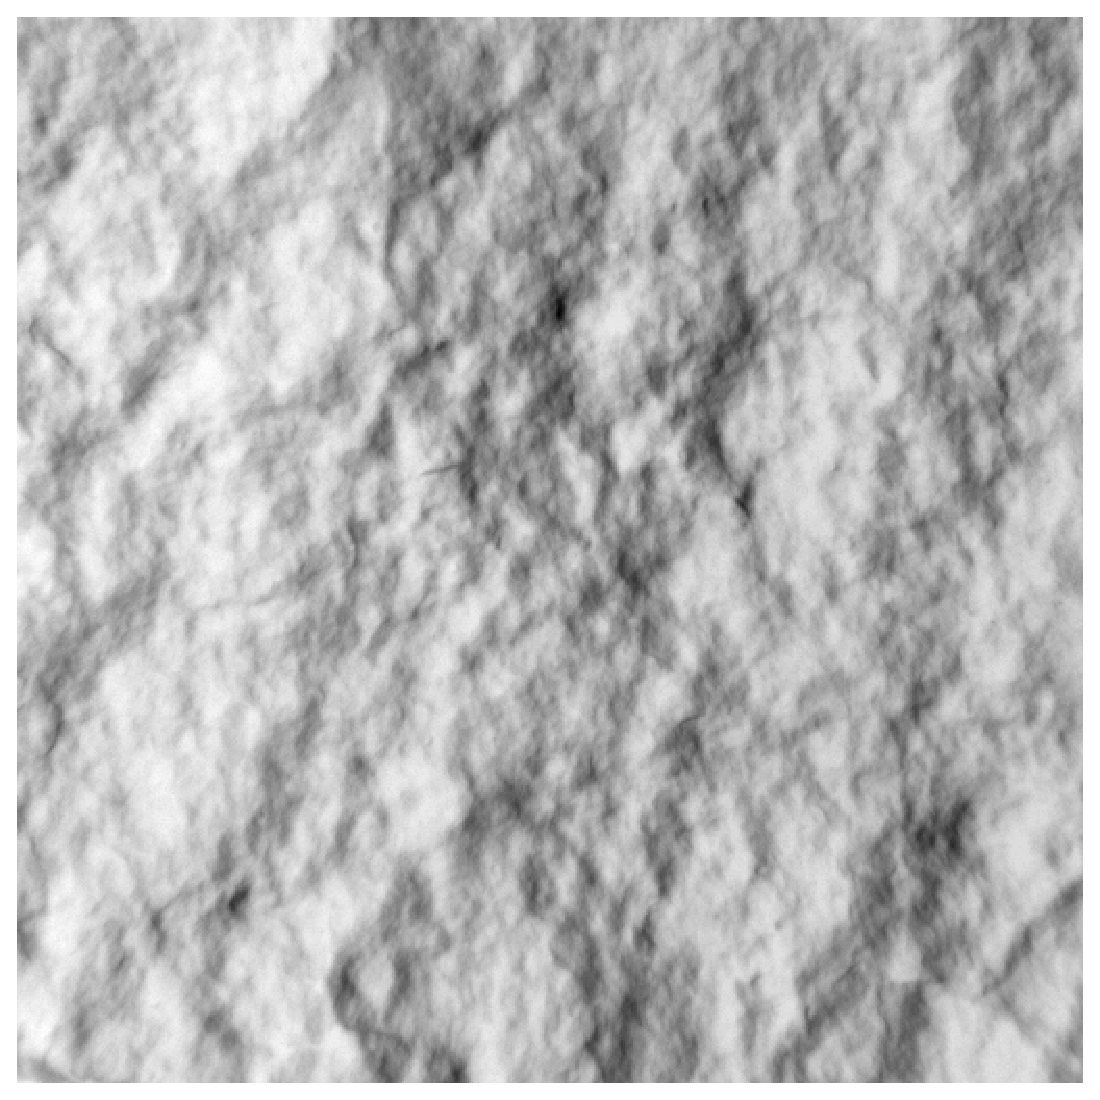
\epsfig{file=images/examples/0.aab.0.30.0.eps, width=0.15\linewidth}}\label{fig:aab1}
		\subfigure[acd]{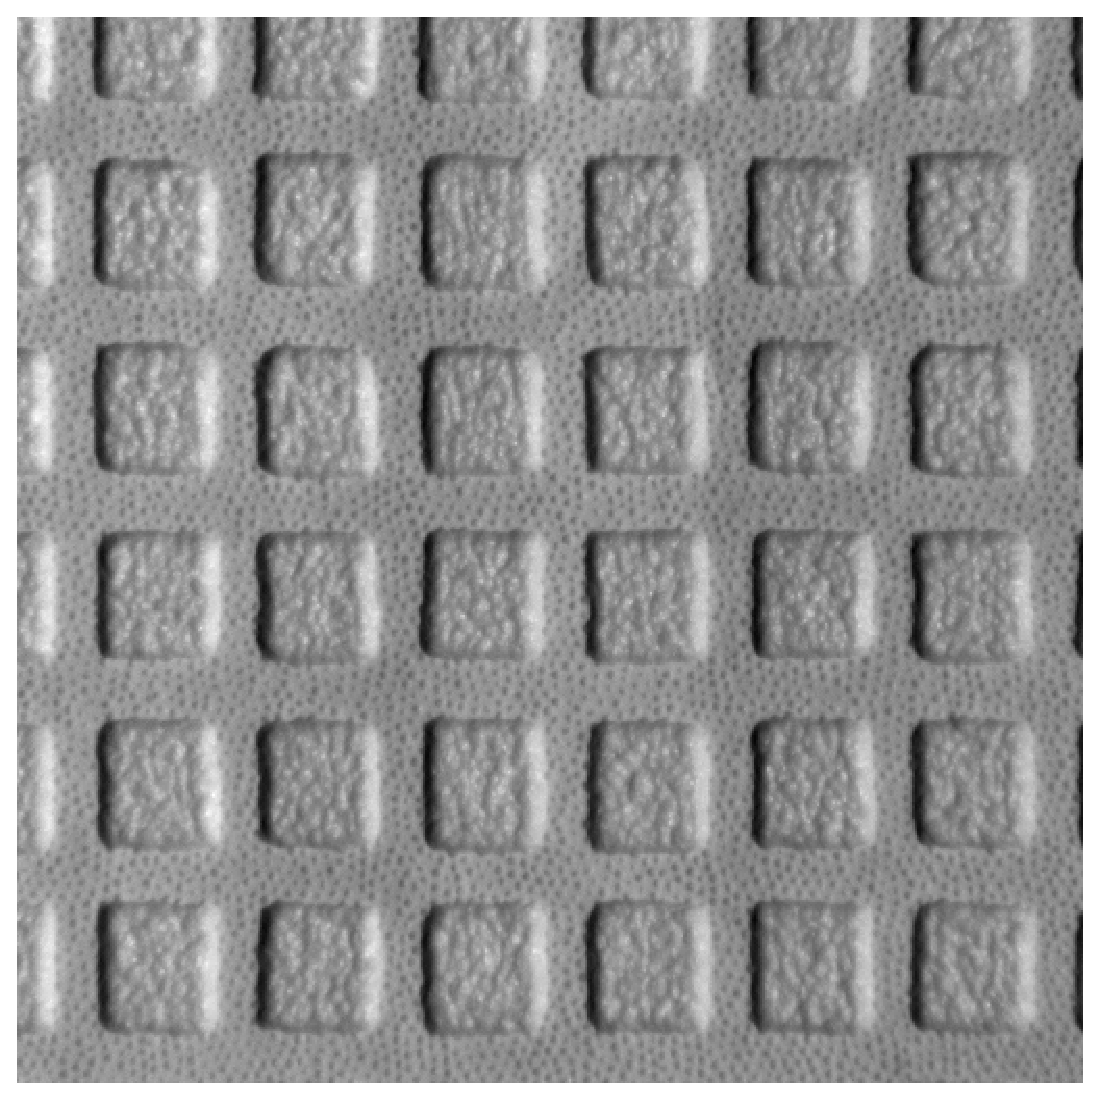
\epsfig{file=images/examples/1.acd.0.30.0.eps, width=0.15\linewidth}}\label{fig:acd1}
		\subfigure[adh]{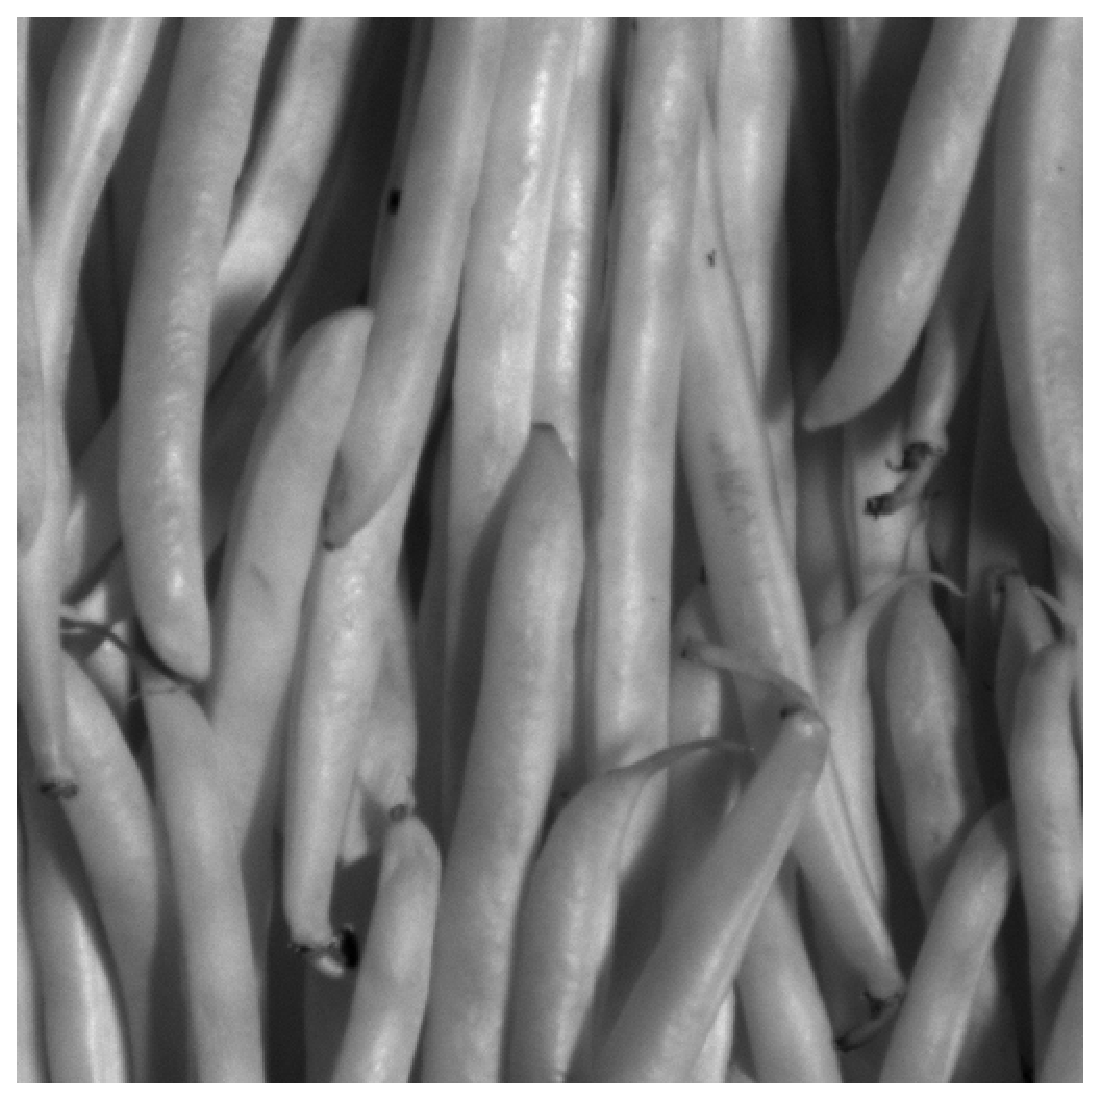
\epsfig{file=images/examples/2.adh.0.30.0.eps, width=0.15\linewidth}}\label{fig:adh1}

		\subfigure[aab]{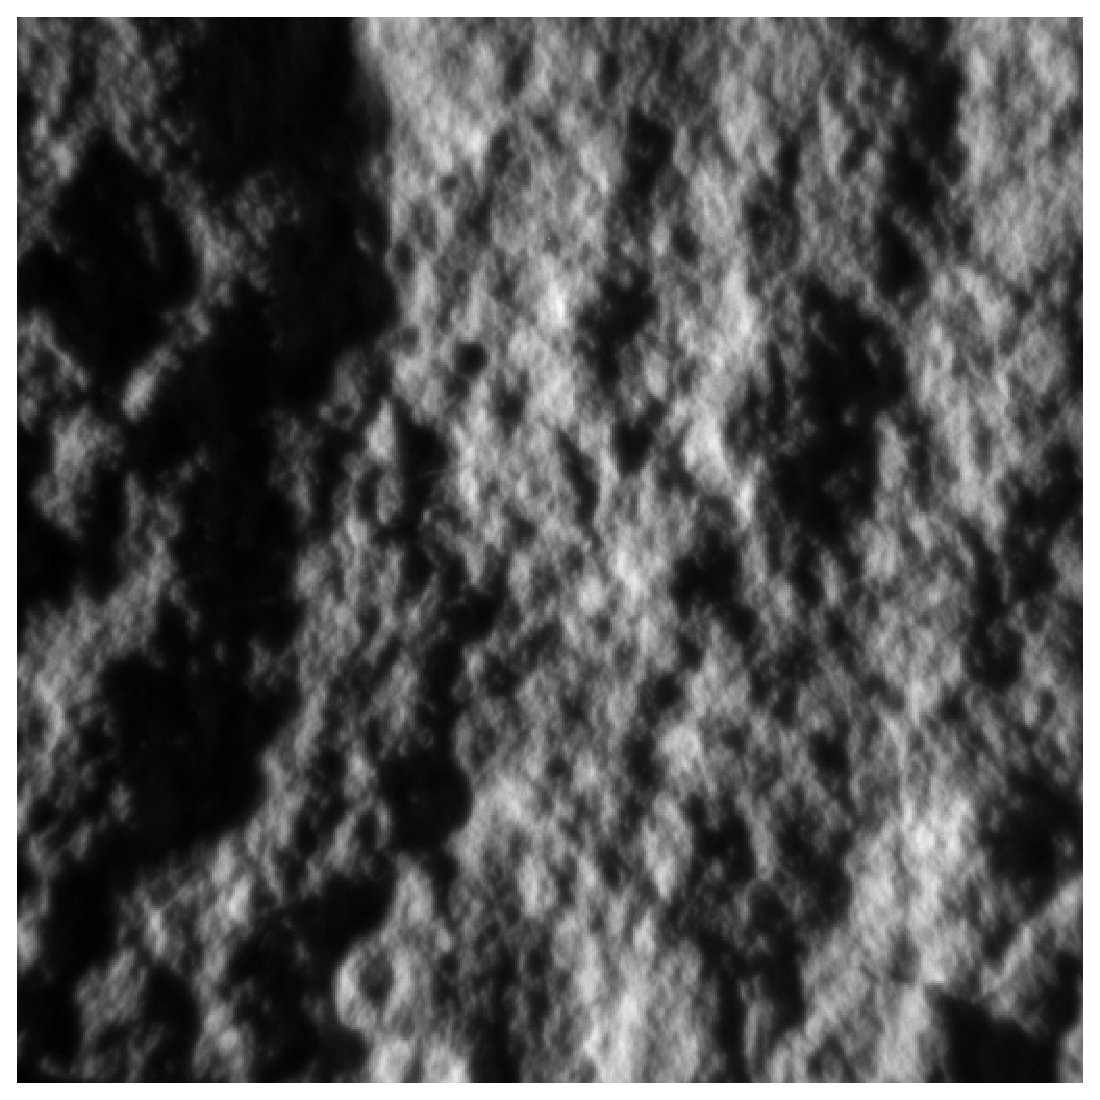
\epsfig{file=images/examples/0.aab.0.75.180.eps, width=0.15\linewidth}}\label{fig:aab2}
		\subfigure[acd]{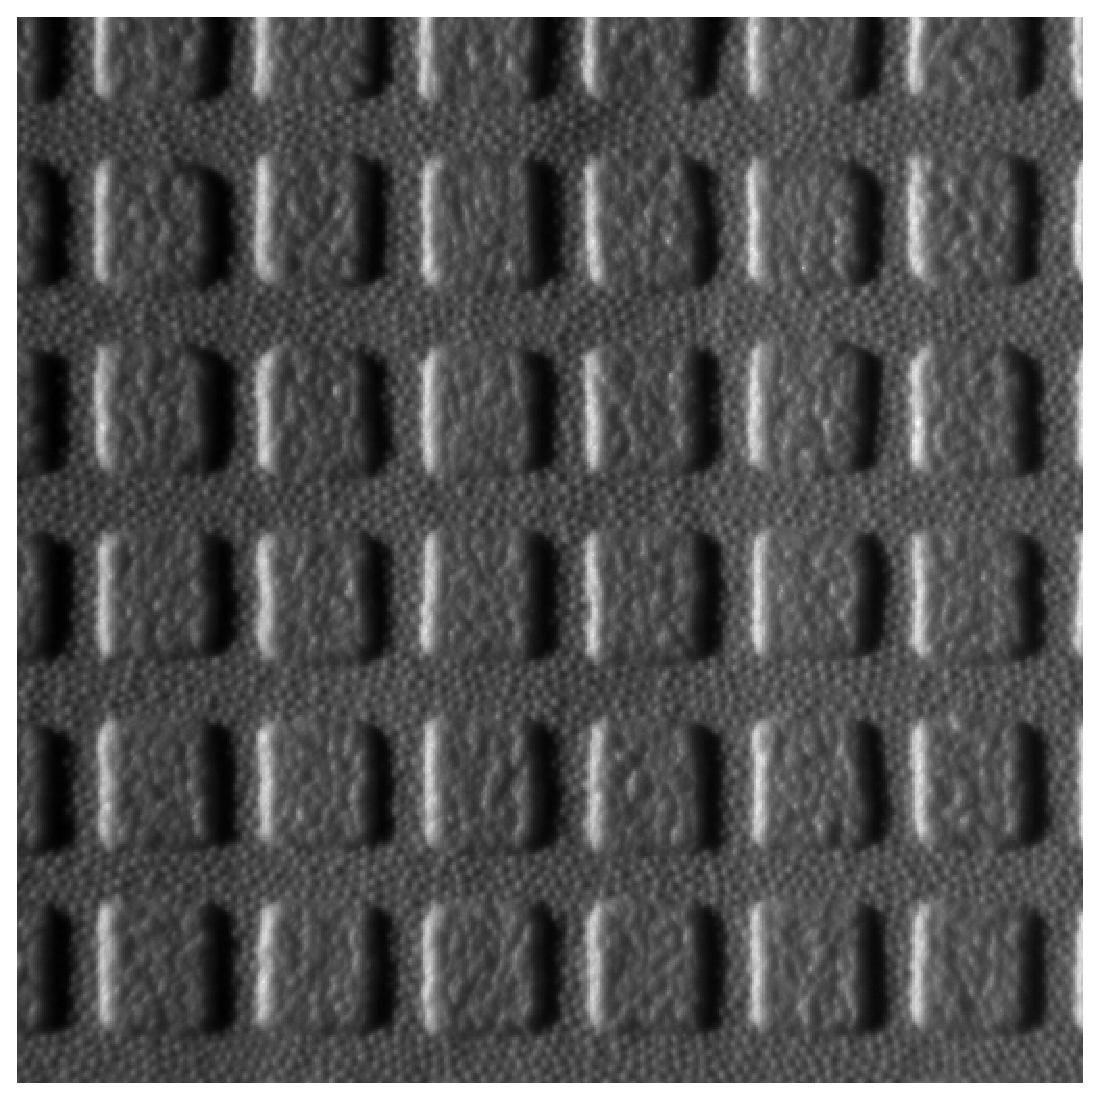
\epsfig{file=images/examples/1.acd.0.75.180.eps, width=0.15\linewidth}}\label{fig:acd2}
		\subfigure[adh]{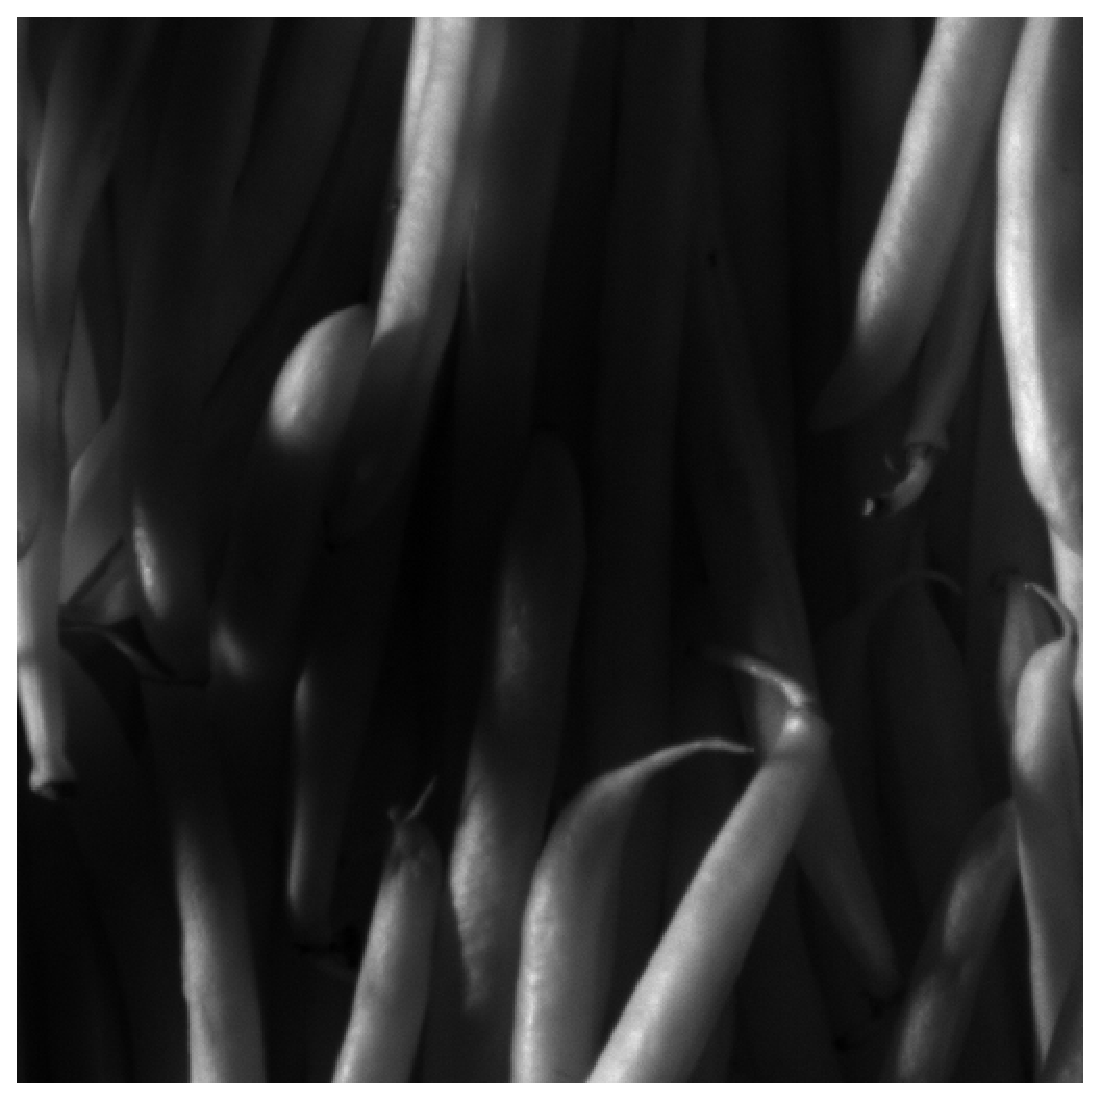
\epsfig{file=images/examples/2.adh.0.75.180.eps, width=0.15\linewidth}}\label{fig:adh2}
	\end{center}
	\caption{{\it Example images from the PhoTex database. The upper row is recorded under a slant of $30^0$ and a tilt of $0^o$. The lower row is recorded under a slant of $75^0$ and a tilt of $180^0$. The captions are the material labels.}}
	\label{fig:PhoTexExamples}
\end{figure}

The {\it CuRET} database captures such properties for 60 different material classes with each over 200 different illumination and viewing directions. This database has been used in the development of texton descriptors to capture the various material properties. In later research on the {\it CuRET} database, parametric models have been developed to deal with the limits of a texton dictionary. The {\it ALOT} and {\it PhoTex} databases have been used in more physically-based computer vision experiments where the geometrical structure of the surface is used for development of robust descriptors. In all these experiments, classification rates of 95\% and higher are reported using various methods such as Naive Bayes, Nearest Neighbor and Support Vector Machines.

The reported classification rates are of great accuracies in general, it seems that most of the difficulties have been solved for material recognition. However, the suggestion that the databases do not capture the intra-class variety for the material classes poses the problem of data shortage. Recording the data is a time-consuming task and will not be sufficiently diverse to capture all possible illumination and viewing directions. 

\section{Image Synthesis}
The field of computer graphics has accomplished imagery of great realism over the past few decades. With increasing computational power, it became possible to synthesize realistic images using expensive physically-based light simulations. 

Various models have been developed for the synthesis of diffuse, glossy or shiny materials. These models use as input for per-pixel generation of an image a surface normal, the surface albedo, a viewing direction, an illumination direction and illumination properties such as the color of the light source. With proper reconstruction of the surface normals and surface albedo for a material, it is possible to generate an infinite amount of data with arbitrary viewing and illumination directions. Databases such as {\it PhoTex} and {\it ALOT} were created with physically-based computer vision in mind. With image data available for each material class with recorded light source directions, it is possible to recover surface normals and surface albedo for material classes. 

In research done by Targhi \cite{Targhi}, the synthesis of material images has been used to augment training-sets to a point of saturation where perfect predictions were made \cite{Targhi}. For the synthesis of image data, the Lambertian reflection model was used. This reflection model is limited to the synthesis of purely diffuse materials only, since the reflection model does not simulate illumination phenomena such as speculars which are observed on glossy and shiny surfaces. Other reflection models should be considered as well if we want to be able to synthesize images for other than purely diffuse materials.

\section{Goal of this thesis}
In this research, the aim is to investigate the addition of more sophisticated reflection models for the synthesis of realistic image data. We research and implement combinations of Lambertian reflectance with models for speculars such as Phong, Blinn-Phong and Torrance-Sparrow, as well as a more sophisticated model for diffuse reflection. 

The synthetic image data is used for training models for material classification. These models are tested against two datasets: a dataset consisting of mainly diffuse materials and a dataset consisting of shiny/glossy materials. Our main focus is to test and compare performance of classification when using only synthetic image data for training the models for classification. With the addition of specular reflection models for synthesis, we can expect some improved models when comparing the performance with models obtained from synthetic data using Lambertian reflection only.

\section{Overview of this thesis}
In the next chapter, some of the state-of-the-art methods and their experiments are outlined. Some of these methods are adapted for the experiments in this research. In chapter 3, the methods that we adapt in this research will be discussed in more detail. Chapter 4 outlines some fundamentals that are used for understanding the reflection models. In chapter 5, a set of empirical reflection models that we implemented for the experiments are discussed in detail. In chapter 6, a set of more physical-based reflection models that we implemented are discussed in detail. In chapter 7, the experiments and their results are reported and the last chapter holds the conclusion and future works.


	\chapter{Related work}
	\hypertarget{RelatedWork}{
}
In earlier research on the topic of material recognition, the main focus was on the albedo variation on top of a flat surface. More recently, this focus has shifted towards surface normals, which cause the $3\mathcal{D}$ effects we perceive in the $2\mathcal{D}$ through shadows and speculars. In this section, three state-of-the-art methods are outlined.

The first method --- presented in section \ref{sec:Textons} --- relies on the construction of a texton dictionary which is afterwards used for feature extraction. The second --- described in section \ref{sec:MGD} --- computes a marginal distribution out of the 8 maximum responses of the convolution of each image with a fixed set of filters. Finally, in section \ref{sec:Minimal} a novel idea is presented in which the performance of a material recognition system is enhances by adding synthetic image data.


\section{Textons}\label{sec:Textons}

The need for larger material databases that capture the variety in viewpoint and illumination resulted in the creation of the {\it CUReT} database. Dana and Nayar \cite{DanaNayar} developed parametric models \todo{based on surface roughness and correlation lengths} which were tested against the {\it CUReT} database. However, in their research, no significant results were reported \cite{VarmaZisserman}.

Leung and Malik were the first to introduce the texton modeling method to the problem of illumination variation \cite{LeungMalik}. In their research, they introduce the concept of 2 and 3-dimensional textons based on Gaussian derivative filters. These Gaussian filters capture certain properties of a material on microscale; for example, a point $n(x,y)$ in an image of a material can correspond to a ridge, bump, groove, spot, etc. A filter-bank of different Gaussian filters can capture these properties in the response of the image applied to such filter. This makes it able to capture the variance of materials under different illuminations using a representable set of filters.

\begin{figure}[b]
	\begin{center}
		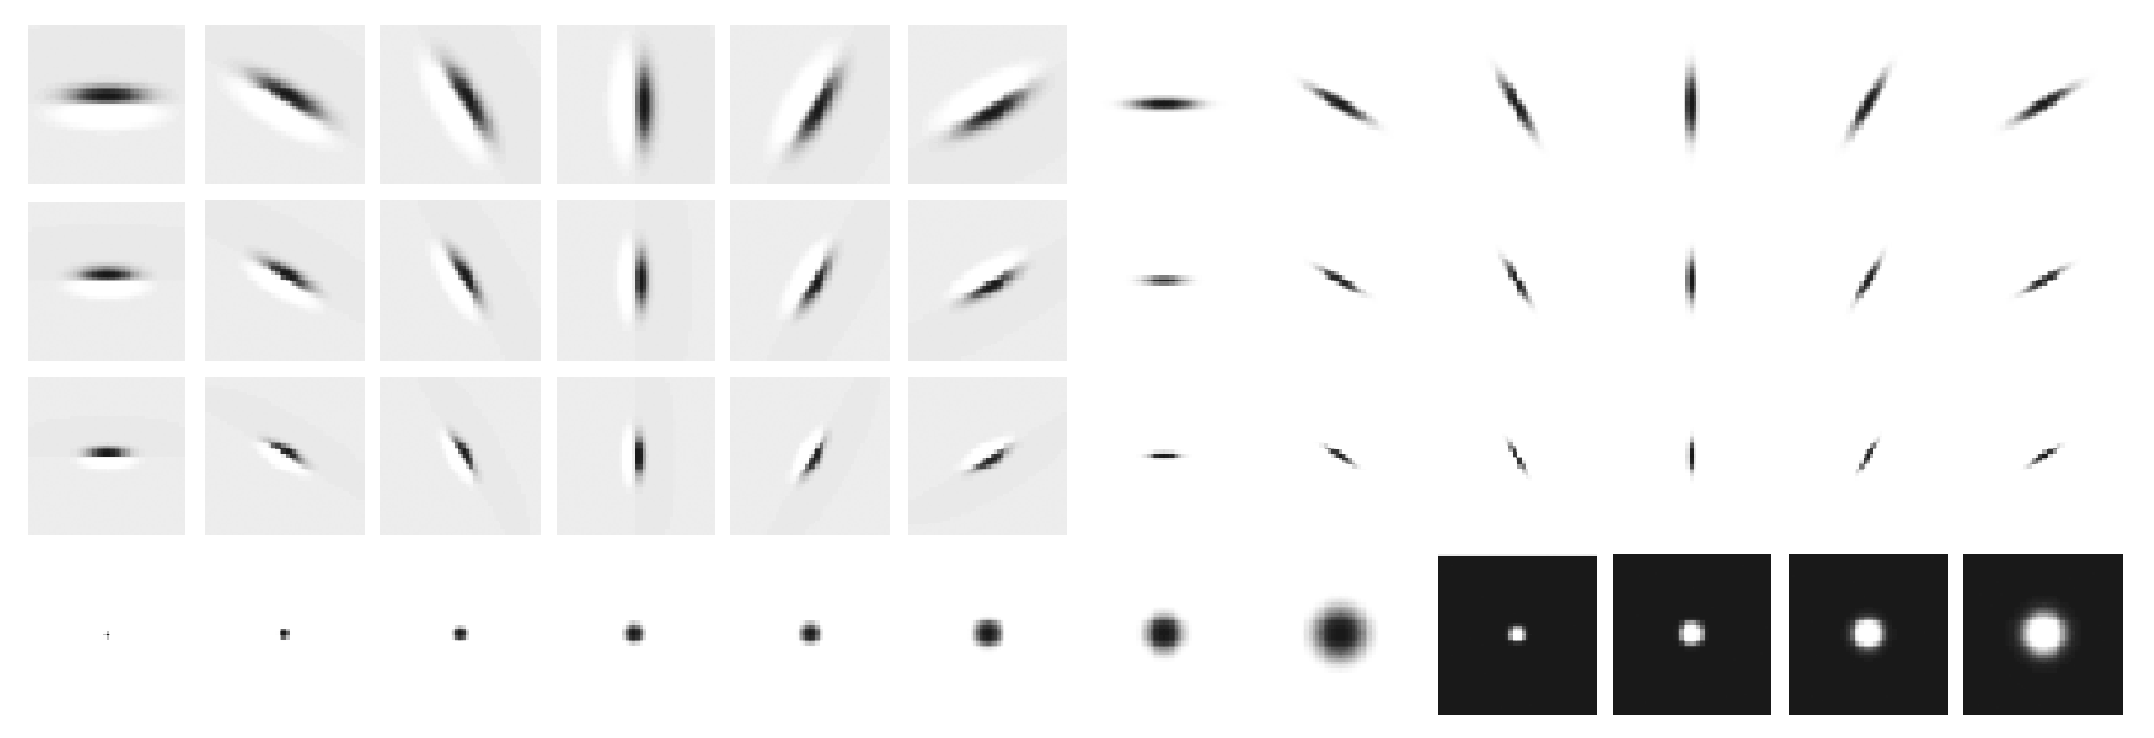
\epsfig{file=images/LM.eps, width=0.6\linewidth}
	\end{center}
	\caption{\textit{LM filter bank, consisting of an edge, bar and spot filter at multiple orientations and scales. 2 Gaussian derivatives at 6 orientations and 3 scales, 8 Laplacian of Gaussian filters and 4 Gaussian filters give a total of 48 filters in the filter bank.}}
	\label{fig:LM}
\end{figure}


In the case of a $2\mathcal{D}$ texton, a material is characterized by responses obtained by convolving images from this material with a set of orientation- and spatial-frequency linear filters. As a result, every pixel in an image is now represented as a vector of $N_{fil}$ corresponding response values, where $N_{fil}$ is the number of filters in the filter bank. With the obtained set of vectors of size $N_{fil}$, they use a K-means algorithm to find a number of vectors as representable clusters in this vector space. The clusters found by K-means give the $2\mathcal{D}$ texton descriptors. These texton descriptors represent characteristics such as ridges, bumps, etc. of the material under a given illumination.

Because a material under a different illumination can appear completely changed due to effects of masking, shadowing, specularity or global illumination, a $2\mathcal{D}$ texton is not enough to capture the general characteristics of a material. As already shown in figure \ref{fig:PhoTexExamples}, the appearance of a material appearances change drastically under different illumination conditions. A great amount of shadows and masking effects make it hard to classify image \ref{fig:PhoTexExamples}(f) when the textons are computed from image \ref{fig:PhoTexExamples}(c), since these effects are not properly quantized by the textons. 

To capture such effects, many images with different illumination variation and viewing directions from the same material are needed. Given a number of images $N_{img} \gg 1$,  concatenating the responses of these $N_{img}$ images will give high dimensional $N_{fil}N_{img}$ data vectors. Clustering these data vectors with K-means will give cluster centers which encode the dominant properties in all the images belonging to a certain material class. These cluster centers represent the $3\mathcal{D}$ textons and encode various image properties like illumination changes, spatial properties (bumps, ridges, etc.), as well as reflectance properties of the material (shiny/glossy as well as diffuse properties). Given the wide range of material characteristics captured by the $3\mathcal{D}$ textons, they represent strong descriptors for the problem of illumination variation within material recognition.

The set of $3\mathcal{D}$ textons --- K-means cluster centers --- over all classes will serve as a texton dictionary for the construction of histograms. Using the same responses as before, for a training image, a histogram is constructed by assigning every vector corresponding to a pixel in the image to a texton in the dictionary using the $\chi^2$ (Chi Square) statistic to measure distance between vector and textons. The histogram is a representation of the image in terms of features, as encoded in the texton dictionary. With this quantization procedure, each material class can be represented by a set of histograms. To classify a novel image, responses are computed, a histogram is constructed using the texton dictionary, and a Nearest Neighbor algorithm is employed to find the histogram in the training set that is closest to it. The function used to measure distances between histograms is again $\chi^2$.

Originally, Leung and Malik used a set of 48 Gaussian derivative filters to compute the responses on an image. Varma and Zisserman extended this research by observing the effect of various filter banks for the computation of the responses \cite{VarmaZisserman}. In their experiments, using a similar setup to that of Leung and Malik, they construct texton dictionaries based on different filter banks and compare performance to the filter bank proposed by Leung and Malik. The filter banks used in these experiments were the Schmid (S) set and the Maximum Response (MR) sets. 

The S set consists of 13 isotropic Gabor-like, rotationally invariant filters. The MR sets consist of 38 Gaussian derivative filters: 2 anisotropic filters for edges and bars, on 6 orientations and 3 scales, and 2 isotropic filters, a Gaussian and a Laplacian of a Gaussian filter. They used two version of this set in their experiments. The MR8 set, only the top 8 responses are recorded by taking the maximum response of the anisotropic filters at each scale over all orientations and taking the responses of both isotropic filters. The MR4 set is a subset of the MR8 set, where the anisotropic filters only occur on a single fixed orientation.

The experiments showed a significant difference in performance for the different filter banks. The best classification accuracy is obtained when using the MR8 filter bank.

\begin{figure}[t]
	\begin{center}
		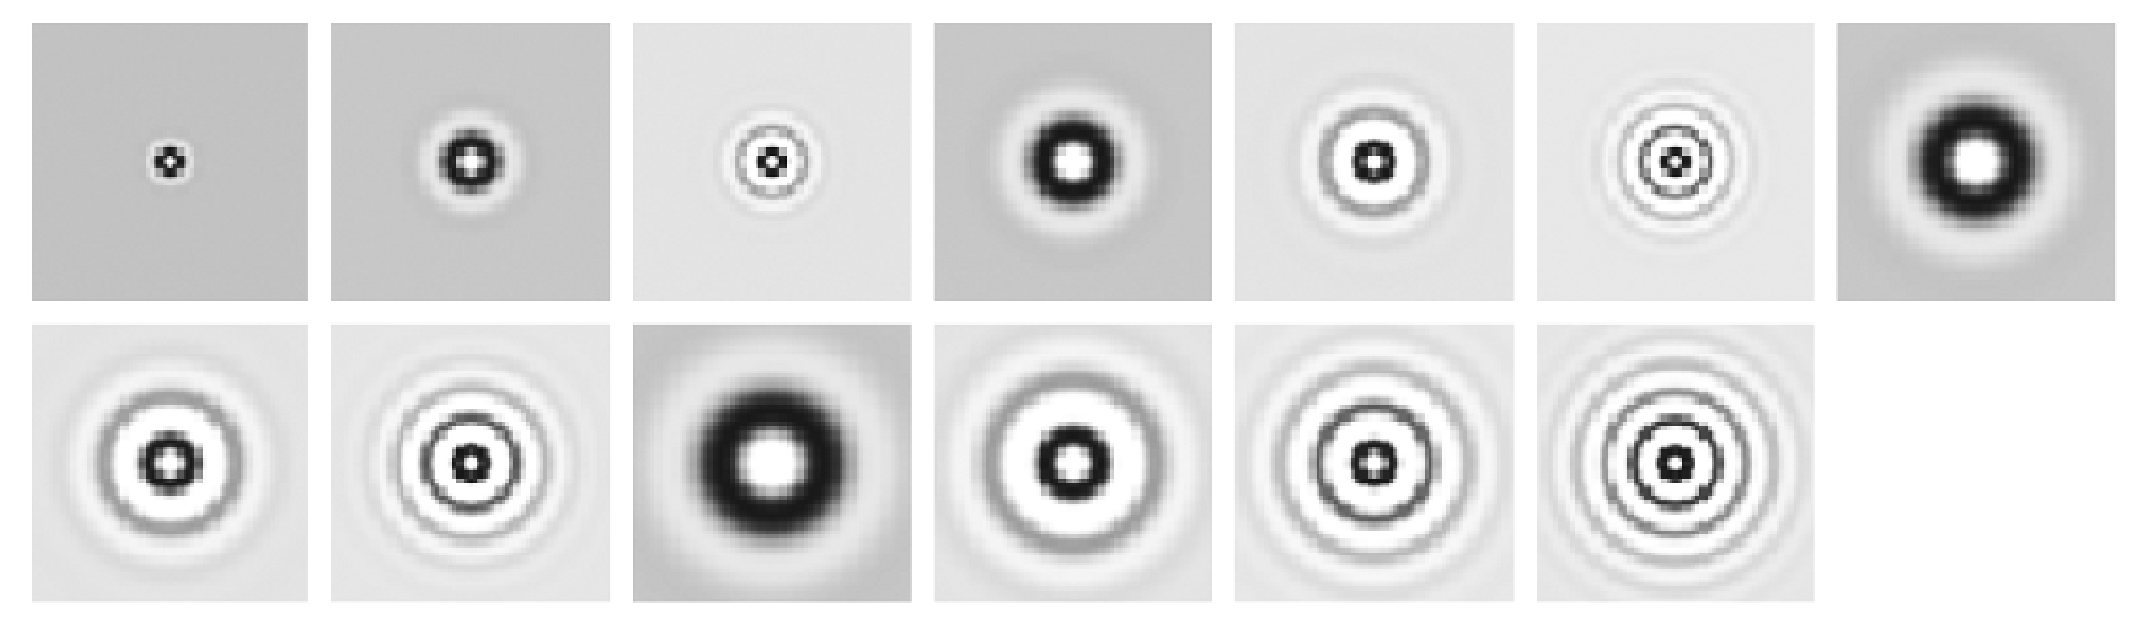
\epsfig{file=images/S.eps, width=0.6\linewidth}
	\end{center}
	\caption{\textit{The Schmid filter bank consists of 13 isotropic rotationally invariant filters.}}
	\label{fig:S}
\end{figure}

\begin{figure}[b]
	\begin{center}
		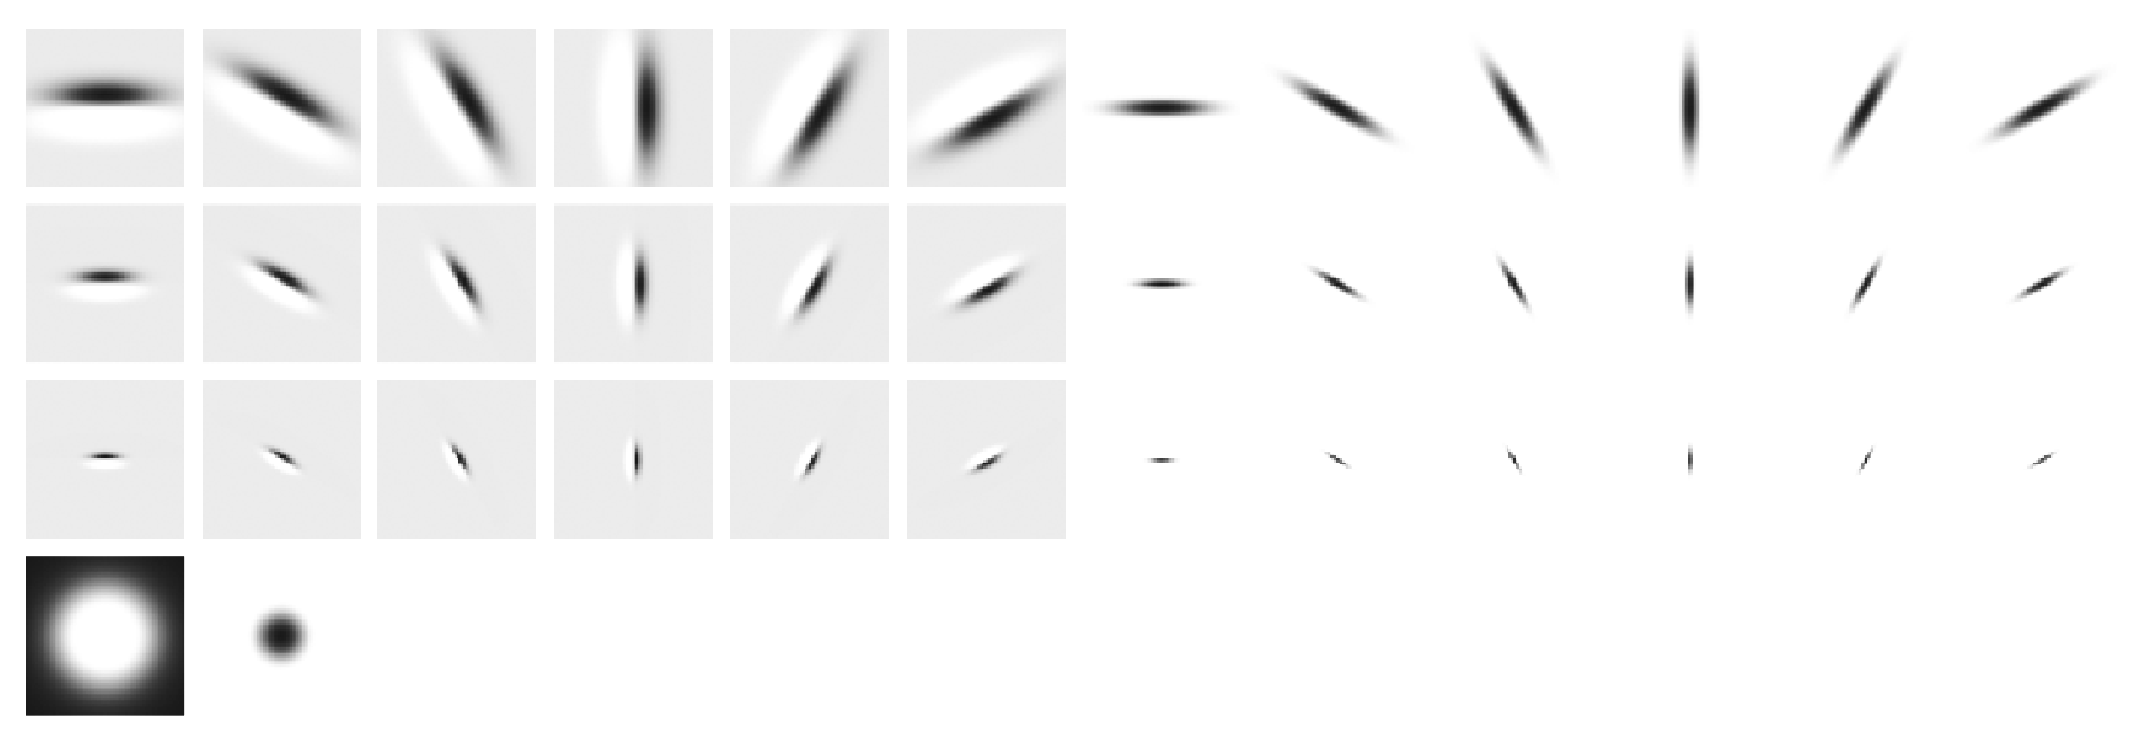
\epsfig{file=images/MR.eps, width=0.6\linewidth}
	\end{center}
	\caption{\textit{The Maximum Response filter bank consisting of 2 anisotropic edge and bar filters at 6 orientations and 3 scales and 2 isotropic filters, a Gaussian and Laplacian of Gaussian. A total of 38 filters, but only 6 filter responses of the anisotropic filters across orientations and the 2 responses of the isotropic filters are registered.}}
	\label{fig:MR}
\end{figure}

\section{Multivariate Gaussian Distributions}\label{sec:MGD}
A drawback of the texton approach is the need for a texton dictionary, which requires clustering in high-dimensional spaces. This poses problems when the number of classes and image data increase as it becomes intractable to compute the clusters. At the same time, the idea of using textons implies that more data is needed to capture general properties that characterizes the data correctly.

Broadhurst presents a parametric approach to estimate the likelihood of homogeneously textured images \cite{Broadhurst}. His work extends the framework proposed by Levina \cite{Levina} by using a Gaussian Bayes classifier instead of a Nearest Neighbor classifier. To model each material class, Broadhurst uses multivariate Gaussian distributions to model the intra-class variability of the marginals within a material class. This is done by constructing marginal histograms out of filter responses, then mapping the joint of the marginal histograms into Euclidean space and applying principal component analysis (PCA) to obtain eigencomponents for each class. With this approach, there is no need for a texton dictionary. The use of a dictionary limits the generalization of a texture class and also needs clustering in high-dimensional spaces, making the problem intractable when extending the number of classes. 

\todo{Although less descriptive than joint conditional distributions, the dependencies among filter responses are captured by estimating the joint intra-class variation of the marginal histograms. This approach increases the descriptive power of the marginal distributions while still maintaining the computational efficiency.}

In order to perform statistical analysis on the marginal distributions, the distributions are mapped to points in Euclidean space. Responses are represented as marginal histograms by sorting the response values in descending order and store the average response value of each bin, creating so-called eqi-count histograms. To compare these discrete distributions, consider two equi-count histograms $x$ and $y$ with $n$ bins and the average value of each bin stored, with their values sorted in descending order. The distributions $x$ and $y$ are represented as vectors of $n$ bin values. The Mallow Distance is used to measure distribution similarity in the Euclidean space. The Mallows distance between these vectors is given by:

	\begin{eqnarray*}
		M_2(x, y) = (\sum^n_{i=1} ||x_i - y_i||)^{1/2}
	\end{eqnarray*}

The described representation maps histograms to points in Euclidean space with distances corresponding to $M_2$ histogram distances. Experiments are run on samples from the {\it CUReT} database, which consists of 61 texture classes with each 205 different viewing and illumination conditions. Each class experiences $3\mathcal{D}$ effect such as interreflections, speculars and shadowing, which gives a large intra-class variability. In a preprocessing step, the images are converted to gray-scale and are processed to have zero-mean and unit-variance to have intensity invariance. The MR8 filter bank is used to gain rotationally invariant features by using the maximum responses over the orientations as done in the works described in \ref{sec:Textons}.

%Levinka has developed a framework for classification using filter banks, marginal histograms, the Mallow distance and a 1NN classifier. The 1-NN classifier requires a distance measure between two sets of marginal distributions. Broadhurst defines this to be the product of the M2 marginal distances described in section 2. The variation of marginal distributions can be measured jointly or independently. A joint 1-NN classifier measures the distance between a target image and all the training images as the distance between each set of marginals. The target image is then classified using the closest training image. For an independent 1-NN classifier, the minimum M2 distance between each target marginal and each class is computed. The total distance to a class is defined as the product of each minimum marginal distance.

In his experiments, Broadhurst considers both independent marginal and joint marginal variation for construction of the Gaussian models. To construct models based on independent marginal variation, eqi-count histograms for each image their 8 maximum responses are computed. The number of histograms chosen in his experiments are 10, 25, 100 and a 1000 bins. PCA is applied to obtain 8 feature specific subspaces per material class, a subspace for each of the filter responses over all training images. For classification, a novel image is projected on the subspaces of each material class and the projection error is computed. The class with the lowest projection error is considered the class of the novel image.

In the experiments conducted by Broadhurst, the joint marginal based models performed significantly better than the independent marginal based models, with $\pm 95\%$ for independent marginals and $\pm 99\%$ for joint marginals. The best performance was measured on histograms with 25 bins.


%After the histograms are computed, PCA is applied to estimate the Gaussian distribution in a lower dimensional subspace for each class and marginal. The number of eigencomponents used differs for the number of bins in the histogram representation, 6, 7, 8 and 9 respectively. As a result, a class is represented by 8 Gaussian models with dimensions equal to the respective number of eigencomponents. 

%For the models based on joint marginal variation, the computed marginals for each image are concatenated into 1 long vector. For each class, PCA is applied on these long vectors to estimate the Gaussian distribution in low dimensional subspace. This gives 1 Gaussian model for each class. To classify novel images, the test image is assigned to the class with the maximum likelihood containing that image. Because all priors are equal for each class, this translates into a Bayes classification problem.


\section{Minimal Training Images}\label{sec:Minimal}

For the construction of models in both methods described in section \ref{sec:Textons} and \ref{sec:MGD}, a lot of image data is required to capture the intra-class variation of the material. This seriously limits the computed descriptors to the amount of illumination and view conditions available in the training data, thus incapable of generalizing effectively beyond the presented data.

In his research, Targhi's central goal is to reduce the amount of images needed for training and yet still produce the same (or better) classification results \cite{Targhi}. With proper reconstruction of surface albedo and surface normals of a material, its possible to generate novel image data with arbitrary viewing and illumination conditions. Using a simple model of photometric stereo, only a small set of original image data is needed for the synthesis of new image data.

For the synthesis of new image data, the Lambertian reflectance model is used. This method effectively simulates diffuse reflection from materials as well as self-shadows, but not more complex light phenomena such as speculars or interreflections. 

Experiments are run on two material databases which are designed for the purpose of physical based texture classification; \textit{ALOT} (\textit{Amsterdam Library of Textures}) and \textit{PhoTex}, a library of photometric image data for texture recognition. The training and testing of the classifier is done by replicating the experiments of Broadhurst. Details on Photex will be outlined in section \ref{sec:PhoTex}. The experimental setup will be described in more detail in section \ref{sec:Experiments}.

Targhi reported improvement over the state-of-the-art results of classification on both databases by augmenting the training data with synthesized data using a minimal amount of images needed for photometric stereo. However, using only the Lambertian reflectance model for image synthesis, it is expected that its application is constrained to diffuse materials. For the synthesis of non-diffuse or non-Lambertian image data, other reflection models are required. More sophisticated reflection models could enhance the quality of the synthetic image data and make it possible to incorporate certain illumination phenomena such as speculars, interreflections and backscattering. 


	\chapter{Approach}
	\hypertarget{Approach}{
\section{Photometric Stereo}\label{PhotometricStereo}
}

\begin{itemize}
	\item{core formula}
	\item{Lambertian assumption}
\end{itemize}

\section{Reflection Models}
\begin{itemize}
	\item{Lambertian}
	\item{Phong, Blinn-Phong}
	\item{Ward}
	\item{Lafortune}
	\item{Microfacets}
	\item{Cook-Torrance}
	\item{Oren-Nayar}
\end{itemize}



\section{Classification}
\begin{itemize}
	\item{multivariate Gaussian Classifier, Mallow distance}
	\item{Texton Dictionary, Chi-distance}
\end{itemize}


	\chapter{Empirical Models}
	\hypertarget{empiricalModels}{
}

%\begin{itemize}
%	\item{Lambertian}
%	\item{Phong, Blinn-Phong}
%	\item{Ward}
%	\item{Lafortune}
%\end{itemize}

\noindent For the texture synthesis of the materials, various local reflection \footnote[1]{Another set of reflection models are global illumination models. These are beyond the scope of this thesis.} models can be used. This chapter will outline the empirical models used in the process of texture synthesis. These models capture reflectance behaviour using mathematical models without using any basic laws of physics. Such models are widely used for their simplicity and because they can be controlled by setting only a small set of parameters to obtain desired results.

\section{Lambertian reflectance}\label{Lambertian}
	One of the most used empirical models is Lambertian reflectance. In computer graphics, this model is mainly used to model diffuse reflectance. Surfaces with such properties appear equally bright from all viewing angles because the light is reflected with equal intensity in all directions. The brightness of the surface is only dependent of the angle $\theta$ between the surface normal $\vec{\mathbf{n}}$ and the light source direction $\vec{\mathbf{l}}$ as shown in figure X. We can look at a diffuse surface on microscopic level to understand how this works. 

If we look at \ref{fig:BEAM}, we can see how an incoming light beam projects a differential area $dA$ on the surface. If the surface normal and the light direction are parallel and in the same direction as shown in figure \ref{fig:BEAM}, the energy the area receives and reflects is proportional to $dA$. If the beam is projected on the surface such that it covers a larger area as shown in \ref{fig:BEAM}, the amount of energy reflected from area $dA$ is proportional to $\cos \theta$. The amount of energy reflected per unit area is less on surface 2 compared to surface 1 since the beam covers a larger area. This observation of radiance behaviour is also known as Lambert's Cosine Law. In general, for Lambertian reflectance, the amount of light observed by the viewer is indepenendent of the viewing angle, and is only dependent on the angle of the incidence of the light source. The full equation is given by:

		\begin{eqnarray*}
			I = I_pk_d\cos\theta
		\end{eqnarray*}

Here, $I$ is the reflected amount of light, $I_p$ is the intensity of the light source, $k_d$ is the \tit{diffuse reflection coefficient} which varies between 0 and 1 and is material dependent. The cosine term is defined between $0^0$ and $90^0$. This means that the surface is treated as self-occluding; angles outside this range will result in negative values for the cosine term and are treated as a $max({0,\cos\theta})$, resulting in zero intensity falling on the surface. If both $\vec{\mathbf{n}}$ and $\vec{\mathbf{l}}$ are normalized, we can write the equation as:

		\begin{eqnarray*}
			I = I_pk_d(\vec{\mathbf{n}} \cdot \vec{\mathbf{l}})
		\end{eqnarray*}

This model is used effectively for the synthesis of diffuse surfaces and in interactive software since the reflection term doesn't need to be recomputed whenever the view changes. However, most materials are deviating from Lambertian for angles of view or incidence greater than $60^0$ \cite{DigitalModeling}. Another shortcoming of Lambertian reflectance is that it does not include the observation of speculars on materials. For these reasons the model is insufficient to synthesize materials with a more glossy nature since they will need the speculars to be present. 


\begin{figure}[H]
	\begin{center}
		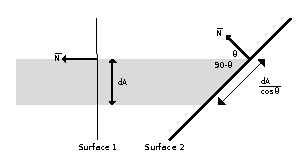
\epsfig{file=images/beam_example.eps, width=0.5\linewidth}
	\end{center}
	\caption{Beam shown in gray, projecting an area on surfaces. The projected area on surface 1 equals $dA$, and on surface 2 equals $\frac{dA}{\cos\theta}$. \tit{Image adapted from Computer Graphics, Principles and Practice \cite{ComputerGraphics}}}
	\label{fig:BEAM}
\end{figure}




	\section{Phong Reflectance}\label{Phong}
		With the Lambertian assumption of light reflecting equally into all direction, we can expect poor quality synthesis when we're dealing with more glossy/specular surfaces such as metallic, stone and plastic materials. As Bui-Tuong Phong wrote in his article, if the goal in shading a computer-synthesized image is to simulate a real physical object, then the shading model should in some way imitate real physical shading situations \cite{Phong}. Phong reflectance is a popular model, based on the empirical observation of how shiny surfaces can have small specular highlights, and how these observed speculars are related to the view direction of the observer.
The general idea of Phong reflection is shown in figure \ref{fig:SPECULAR1}. Here we have an incident angle $\theta_i$ and an equal reflection angle $\theta_r$. The angle between $\vec{\mathbf{r}}$ and $\vec{\mathbf{v}}$, $\alpha$, defines how strong a specular is perceived by the observer. If this angle is zero (ie. the reflection- and view-direction are in the same direction), the perceived intensity will be maximal. When this angle increases, the observed intensity of the specular will fall off fast.

\begin{figure}[H]
	\begin{center}
		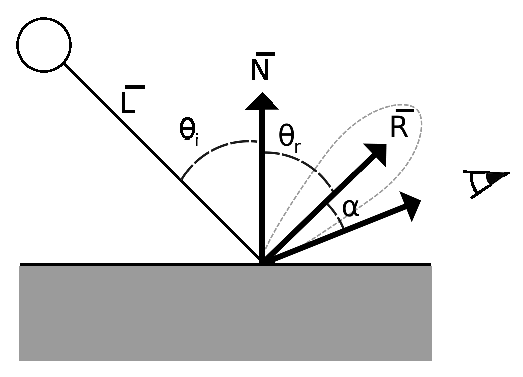
\epsfig{file=images/specular_reflection.eps, width=0.4\linewidth}
	\end{center}
	\caption{Specular reflection. $\theta_i$ is the angle of the incoming light, and is equal to the reflected angle $\theta_r$. $\alpha$ is the angle between the view direction and the reflected light.}
	\label{fig:SPECULAR1}
\end{figure}


\noindent The reflection model is computed as:

	\begin{eqnarray*}
		I = i_a + k_d(\vec{\mathbf{l}} \cdot \vec{\mathbf{n}}) + k_s(\vec{\mathbf{r}} \cdot \vec{\mathbf{v}})^\alpha
	\end{eqnarray*}

\begin{itemize}
	\item[] $i_a$ is a parameter controlling the ambient lighting.
	\item[] $k_d$ is the diffuse reflection coefficient.
	\item[] $k_s$ is the specular reflection coefficient.
	\item[] $\vec{\mathbf{l}}$ is the direction vector for the light source.
	\item[] $\vec{\mathbf{v}}$ is the direction vector for the observer.
	\item[] $\vec{\mathbf{n}}$ is the surface normal.
	\item[] $\vec{\mathbf{r}}$ is the direction vector for the reflected light, 
		calculated as $2\vec{\mathbf{n}}(\vec{\mathbf{l}} \cdot \vec{\mathbf{n}}) - \vec{\mathbf{l}}$
	\item[] $\alpha$ is a parameter controlling the specular size, also known as the shininess constant, which is material-dependent. The greater $\alpha$ is, the smaller the size of the specular.
\end{itemize}

Here, the parameterse $k_d$ and $k_s$ are constants for diffuse and specular reflection respectively. 
This formula is simplified such that it doesn't involve more than one light source. More light sources could be incorporated easily by computing the diffuse and specular components for each light source separately and summing these to obtain the total contribution. With respect to the experiments, multiple light sources are not necessary. Also, the components defining colors are left out since we're only concerned about grayscale images in the experiments. The ambient term can be left out as well, since a preprocessing step will make the synthesized images intensity-invariant. A common complaint about the Phong model is that it is completely emperical, and doesn't abide the most basic law in physics - the conservation of energy. Appropriate normalization factors could be applied to constrain the model to this law.

	\section{Blinn-Phong Reflectance}\label{BlinnPhong}
		Short after Phong published his model, Blinn proposed an alternative to compute the specular component where the angle $\theta_s$, dot product between the reflection vector and viewing vector, could be replaced by $\theta_h$ \cite{Blinn}. This angle the dot product between the normal of the surface, and the so called halfway-vector $\vec{\mathbf{h}}$. This halfway-vector is the bivector between the light source vector $\vec{\mathbf{l}}$ and the view direction vector $\vec{\mathbf{v}}$, and is computed as:

	\begin{eqnarray*}
		\vec{\mathbf{h}} = \frac{\vec{\mathbf{l}} + \vec{\mathbf{v}}}{|\vec{\mathbf{l}} + \vec{\mathbf{v}}|}
	\end{eqnarray*}

He observed that mirror reflections only occur when the surface normal is aligned with the halfway-vector \cite{DigitalModeling}. When observing a material with glossy/shiny properties, the microscopic structure of the material is never entirely smooth and can be illustrated as microscopic small surfaces. The main normal of the surface is still $\vec{\mathbf{n}}$, but each micro-surface has its own surface normal as well. The distribution of the specular lobe can be expressed as the amount of microfacets with normals aligned with the halfway-vector, with a likelihood related to $\theta_h$.

Replacing $\theta_s$ with $\theta_h$ doesn't give the same reflectance function as with Phong reflection, and as a result it produces slightly different speculars. However, because of computational convenience, Blinn-Phong reflectance is being used in most systems these days.

	\chapter{Microfacet Models}
	\hypertarget{Microfacet Models}{
}

\noindent In the previous section, the reflection models were based on empirical observations. Research in optics found that these models deviate from reality in a number of aspects. In this section, a more physically correct class of reflection models will be outlined. They are called \textit{first principles} models because they apply basic laws of physics on a microscopic scale. The interaction of light on this microscopic scale in turn determines how the light gets reflected from the surface. The light interaction could be described by either wave or geometric optics, but only geometric optics based models are discussed in this research.

The models described here start by modeling the surface geometry at microscopic scale. Rather than providing an exact description of this structure, the assumption is made that the surface varies randomly in height and orientation of facets. With this assumption, its possible to use statistical models to model surface structures.

\section{Surface Roughness Model}
There are two possible methods to represent the random surface. Both methods use small differently oriented areas in their representation, also called microfacets. The first method is to model the surface using a random process such as described by Beckmann and Spizzichino \cite{BeckmannSpizzichino}. They suggest to build the surface by using coin-flipping a procedure to decide to increase, decrease one or two units or stay on the same level. Although the resulting surface will have a desirable randomness, it is very complex to derive reflectance models using this method. 

The second method uses distributions of primitive shapes to represent the surface. Asserting the assumption $\lambda^2 \ll da \ll dA$, where wavelength of light $\lambda$ is much smaller than the facet area $da$, and the facet area $da$ is much smaller than the area $dA$ (which is a pixel on the surface), geometric optics can be used to derive the reflectance models. 

Torrance and Sparrow suggested to represent the surface as a composition of symmetric V-cavities, where each microfacet has a height much bigger than their width and the upper edges are all laying in the same plane.

\section{Geometric Optics}ImprovedDiffuse
The idea of describing the surface as a collection of microfacets is originally developed in the field of optics and radiation transfer. Microfacets with respect to computer graphics has first been addressed by Blinn \cite{Blinn}. He proposed that a model for computer simulation could be composed from the following factors:

\begin{itemize}
	\item{ The number of microfacets are facing the orientation of the viewing direction, and what is the projected area of the facets into the viewing direction. This is computed by the slope distribution function. }
	\item{ How much incoming light on a microfacet gets blocked by other microfacets, causing shadows to appear on the blocked microfacet when observing the microfacet from certain angles (see figure X).} 
	\item{ How much reflected light into the viewing direction gets blocked by other microfacets, causing the amount of radiance reaching the viewer to be smaller than the amount of radiance that gets reflected from the microfacet. This phenomenon is called masking, and is also shown in figure X. }
	\item{ How much can an unobstructed microfacet reflect? This is mainly dependent on a given reflectance function for the microfacet. This is general is either Lambertian or pure specular. See figure X for an example using pure specular reflectance}
\end{itemize}

The shadowing and masking of the microfacets need additional geometric analysis next to the slope distribution. The most common way to deal with this analysis is to assume that the microfacets form V-shaped cavities as shown in the example images. This approach has been challenged since the assumption is inconsistent with the assumption of a random looking surface, but it makes geometric analysis much easier.

Another case of geometric analysis which can be included, is the phenomenon of interreflection. This happens when radiance is being exchanged between two diffuse surfaces, and causes the effect of color bleeding. The analysis is included in the reflection model proposed by Oren and Nayar, and is described in section \ref{sec:OrenNayar}.

\begin{figure}[H]
	\begin{center}
		\subfigure[Unblocked]{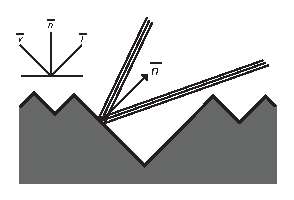
\epsfig{file=images/MicroNoObstruction.eps, width=0.4\linewidth}}
		\subfigure[Shadowing]{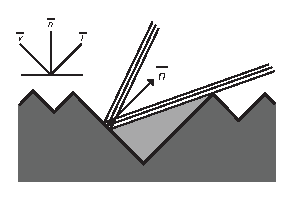
\epsfig{file=images/MicroShading.eps, width=0.4\linewidth}}
		\subfigure[Masking]{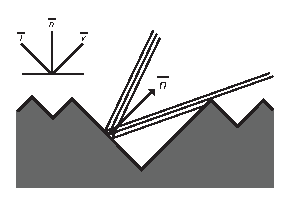
\epsfig{file=images/MicroMasking.eps, width=0.4\linewidth}}
		\subfigure[Interreflection]{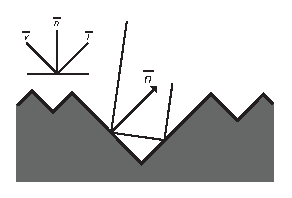
\epsfig{file=images/MicroInterreflection.eps, width=0.4\linewidth}}
	\end{center}
	\caption{Four cases of light interaction on microfacets.}
	\label{fig:GAF}
\end{figure}


\section{Torrance-Sparrow Reflectance}\label{sec:CookTorrance}
	The results of experiments conducted by Sparrow and Torrance \cite{TorranceSparrow} showed that Phong reflectance does closely simulates the behavior of the specular component on shiny/glossy surfaces. However, some differences were reported, with the main difference being that the specular bump varies with the direction of the light source. Also, the specular reflection is not always reflected in the halfway vector H. 

Torrance and Sparrow derived models to explain these differences, and Blinn translated these models to be useful in computer graphics. The specular component can be described as a function of four factors: 
	
	\begin{eqnarray*}
		f_r = \frac{F(\theta_h)D(\theta_h)G(\theta_i,\theta_r)}{\vec{\mathbf{n}} \cdot \vec{\mathbf{e}}}
	\end{eqnarray*}

\noindent where $D$ is the distribution function of the directions of the microfacets. Each microfacet is assumed to be perfectly specular. $G$ contributes the amount of light that gets masked and/or shaded by other microfacets, and $F$ is the Fresnel reflection law.

Taking into account that the observer sees more of the microfacet surface area when the surface is tilted, this tilt angle is included in the division in the above equation as $\vec{\mathbf{n}} \cdot \vec{\mathbf{e}}$, since this observed area is inversely proportional to the cosine of the tilt angle.

The distribution function used by Torrance and Sparrow was a simple Gaussian function, $D = e^{-(\alpha c)^2}$, where $c$ is the standard deviation and $D$ is the amount of microfacets oriented at an angle $\alpha$, the angle between the facing direction of the microfacets and the surface normal. Since we are only interested in the microfacets pointing into the direction of $\vec{\mathbf{h}}$, the angle $\alpha = \theta_h$. Blinn used a different function however, developed by Trowbridge and Reitz, and suggests modeling the microfacet distribution as ellipsoids:

	\begin{eqnarray*}
		D_{Blinn}(\theta_h) = \left({ \frac{m^2}{\cos^2(\theta_h)(m^2-1)+1} } \right)^2
	\end{eqnarray*}

\noindent In the above equation, the parameter $m$ controls the eccentricity of the ellipsoid. When set to 0, the distribution defines a shiny surface, and when set to 1, it defines a rough surface.

The factor $G$ in the specular reflection equation accounts for the effect of masking and shadowing of microfacets. This factor is also called the \textit{geometrical attenuation factor}, and gives a value between 0 and 1 to represent the amount of light remaining after shadowing/masking. The method described by Blinn to calculate this factor assumes symmetrical identical V-shaped cavities as stated earlier. 

The three cases are included in the geometrical attenuation factor. For arbitrary light source directions and viewing directions, the three cases that can happen are shown in figure \ref{fig:GAF}.

The first case is that of figure \ref{fig:GAF}a, where no light is obstructed by other microfacets and therefore there is no attenuation. In this case, the attenuation is defined as:

	\begin{eqnarray*}
		G_a = 1
	\end{eqnarray*}

In the case of figure \ref{fig:GAF}b, some of the incident light gets intercepted when traveling to the observer. For this case, the attenuation is defined as follows:

	\begin{eqnarray*}
		G_b = \frac{2\cos(\theta_h)\cos(\theta_r)}{\cos(\theta_{rh})}
	\end{eqnarray*}

\noindent Because the same concept applies for figure \ref{fig:GAF}c, but the light and view source are interchanged, the final attenuation can be defined as:

	\begin{eqnarray*}
		G_c = \frac{2\cos(\theta_h)\cos(\theta_i)}{\cos(\theta_{rh})}
	\end{eqnarray*}

\noindent For the exact derivation of these individual terms, the work of Blinn \cite{Blinn} can be consulted. For the implementation of $GAF$, the minimum of all three cases is used as the effective value for $G$:

	\begin{eqnarray*}
		G = min \left[ {G_a, min \left[ {G_b, G_c} \right] } \right]
	\end{eqnarray*}

\noindent The final term in the specular reflection equation is the Fresnel term. This term gives the fraction of light that is reflected from a microfacet instead of being absorbed. An object's surface is considered an interface between two different substances; the object's substance and the substance the object is surrounded with (eg. water or in this case air). The Fresnel equations, developed by Augustin-Jean Fresnel in the 19th century, describe an optical property such that reflected light is not only dependent on the incoming light angle $\theta_i$, but also on the \textit{refraction index} of both substances. The exact Fresnel equations are quite complex and need correct refraction indices which are not available for the PhoTex database. 

A simplified version of the Fresnel equations is given by Schlick \cite{Schlick}, which is proven to be fairly accurate for a lot of substances and is given by the equation:

	\begin{eqnarray*}
		F(\theta_i) = R_f(0^o) + (1 - R_f(0^o))(1 - \cos(\theta_i))^5
	\end{eqnarray*}

\noindent in this equation, $R_f(0^o)$ represents the specular color of a substance when the incident light strikes the surface under an angle of $\theta_i = 0$. This value for $R_f(0^o)$ is typically low for dielectrics such as plastic, stone, wood, concrete, leather, etc. and is measured around 0.05 or lower \cite{RTR}. 


\section{Oren-Nayar Reflectance}\label{sec:OrenNayar}
A big deficiency in approximating the body reflectance under the Lambertian assumption is that its view independent. This results in inaccurate approximations for several real-world objects, as experiments have demonstrated on rough diffuse surfaces such as plaster, sand and clothing \cite{OrenNayar}. The main issue with Lambertian reflection for diffuse objects is that it creates high contrasts around the occluding boundaries of an object (such as a clay vase). \todo{Figure \ref{fig:OrenNayarExplained}} explains with the use of microfacets why the occluding boundaries created by Lambertian reflectance tend to be too dark.

To overcome this deficiency, M. Oren and S.K. Nayar propose a more general reflection model for diffuse surfaces \cite{OrenNayar} \cite{ImprovedDiffuse}, which borrows ideas from modeling the surface as a collection of microfacets as proposed for the Cook-Torrance or Torrance-Sparrow models. Microfacets are assumed to be perfectly Lambertian in reflection. This does not imply that surfaces are reflecting perfectly Lambertian however, since combination of all factors included produces accurate diffuse reflection also for non-Lambertian diffuse surfaces. 

The general form of the equation consists of two part:

	\begin{eqnarray*}
		f_r = f_r^1 + f_r^2
	\end{eqnarray*}

\noindent The first part of the equation, $f_r^1$ accounts for the amount of radiance that is projected on the facets, and includes analysis for the geometric attenuation factor. The second part, $f_r^2$ accounts for radiance caused by interreflections.

%In their original paper, Oren and Nayar discussed various slope distributions for the distribution of of microfacets. Using an uni-directional single-slope distribution (representing an anisotropic surface), they derive a geometric attenuation factor similar to that derived by Torrance and Sparrow. Their analysis continues by considering distributions for isotropic surfaces. However, those distribution models assume equal slopes for all microfacets, which isn't realistic. 

For the modeling of a surface, they propose to use a Gaussian Slope-Area distribution $P(\phi_a, \theta_a)$, where the parameter $\theta_a$ is the standard deviation, and is a measurement for the roughness of the material. Because evaluating the complete integral using the Gaussian Slope-Area distribution turned out too difficult, approximations of this integral were made using numerical evaluations. The resulting equations are therefore not a result of analysis:

	\begin{eqnarray*}
		f_r^1 = \frac{\rho}{\pi}L_i\cos(\theta_i)\left[C_1+\cos(\phi_r-\phi_i)C_2\tan(\beta) 
			  + (1-|\cos(\phi_r-\phi_i)|)C_3\tan\left(\frac{\alpha+\beta}{2}\right)\right]
	\end{eqnarray*}

\noindent with the coefficients defined as:

	\begin{eqnarray*}
		C_1 = 1 - 0.5\frac{\sigma^2}{\sigma^2+0.33}
	\end{eqnarray*}

	\begin{eqnarray*}
		C_2 =
			\begin{cases}
				0.45\frac{\sigma^2}{\sigma^2+0.09} 		& \quad \text{if $\cos(\phi_r - \phi_i) \geq 0$}\\
				0.45\frac{\sigma^2}{\sigma^2+0.09} \left( \sin(\alpha) - \left( \frac{2\beta}{\pi}\right)\right) 	& \quad \text{otherwise}\\
			\end{cases}
	\end{eqnarray*}

	\begin{eqnarray*}
		C_3 = 0.125 \left( \frac{\sigma^2}{\sigma^2+0.09} \right)\left( \frac{4\alpha\beta}{\pi^2} \right)
	\end{eqnarray*}

\noindent Since the energy of a light ray diminishes quickly on Lambertian surfaces, they consider interreflection up to two bounces. The same approach of finding a good approximation accounts for defining the interreflection term:

	\begin{eqnarray*}
		f_r^2 = 0.17\frac{\rho^2}{\pi}L_i\cos(\theta_i)\frac{\sigma^2}{\sigma^2+0.13}\left[1-\cos(\phi_r-\phi_i)\left( \frac{2\beta}{\pi} \right)^2 \right]
	\end{eqnarray*}

\noindent A more simplified version was proposed by the authors, leaving out the interreflection term, since the above equations are too complex to apply in rendering software in general. In this research however, the experimental setup for finding good parameter settings showed that the error in image quality is significantly smaller than when using the simplified equations. For this reason, the choice was made to use the original model for Gaussian Slope-Area distribution.




	\chapter{Experiments}
	\hypertarget{experiments}{
}

In the experimental stage of this research, two experiments are performed on two different datasets to analyse the overall quality of the synthesized data. The experiments conducted by Targhi for diffuse material classes are replicated and extended with synthesis using other reflection models, and the same setup is used on a new selection of material classes from the {\it PhoTex} database. The new selection of material classes have more glossy/shiny properties unlike the classes selected by Targhi, which should give a better indication for the quality of specularity simulated by Phong, Blinn-Phong and Torrance-Sparrow reflectance. 

\section{Preprocessing}\label{sec:preprocessing}
The {\it PhoTex} database consists of images recorded under a fixed point of view with varying light-source directions registered for each image. For the experiments, two datasets are chosen: a dataset according to the selection made by Targhi and another dataset with shiny properties to extend the experiments for the specular reflection models. 

After rendering new images for the materials and before extracting the features from the materials, the rendered images are set to zero-mean and unit-variance in order to make the features intensity-invariant. Since the diffuse and glossy/shiny materials have different image sizes, all images are cropped with respect to the center of the image to $200 \times 200$ pixels.

\subsection{Diffuse material classes}
Since we are interested in reproducing some results from the experiments of Targhi, and measure performance of more complex reflection models with respect to the Lambertian reflection model he applied, we need to select the same material classes he used in his experiment. These material classes are shown in figure \ref{fig:PhoTexData}.

From each material class, 40 images with certain slant and tilt angles are selected. The selected slant angles are $\{30^0, 45^0,60^0,75^0\}$. The images under a slant of $30^0$ have four different tilts, $\{0^0, 90^0, 180^0, 270^0\}$. The images with slants $\{45^0,60^0,75^0\}$ have tilts of $\{0^0,30^0,60^0,..., 300^0,330^0\}$. 

%\begin{comment}
\begin{figure}[h]
	\begin{center}
		\subfigure[aaa]{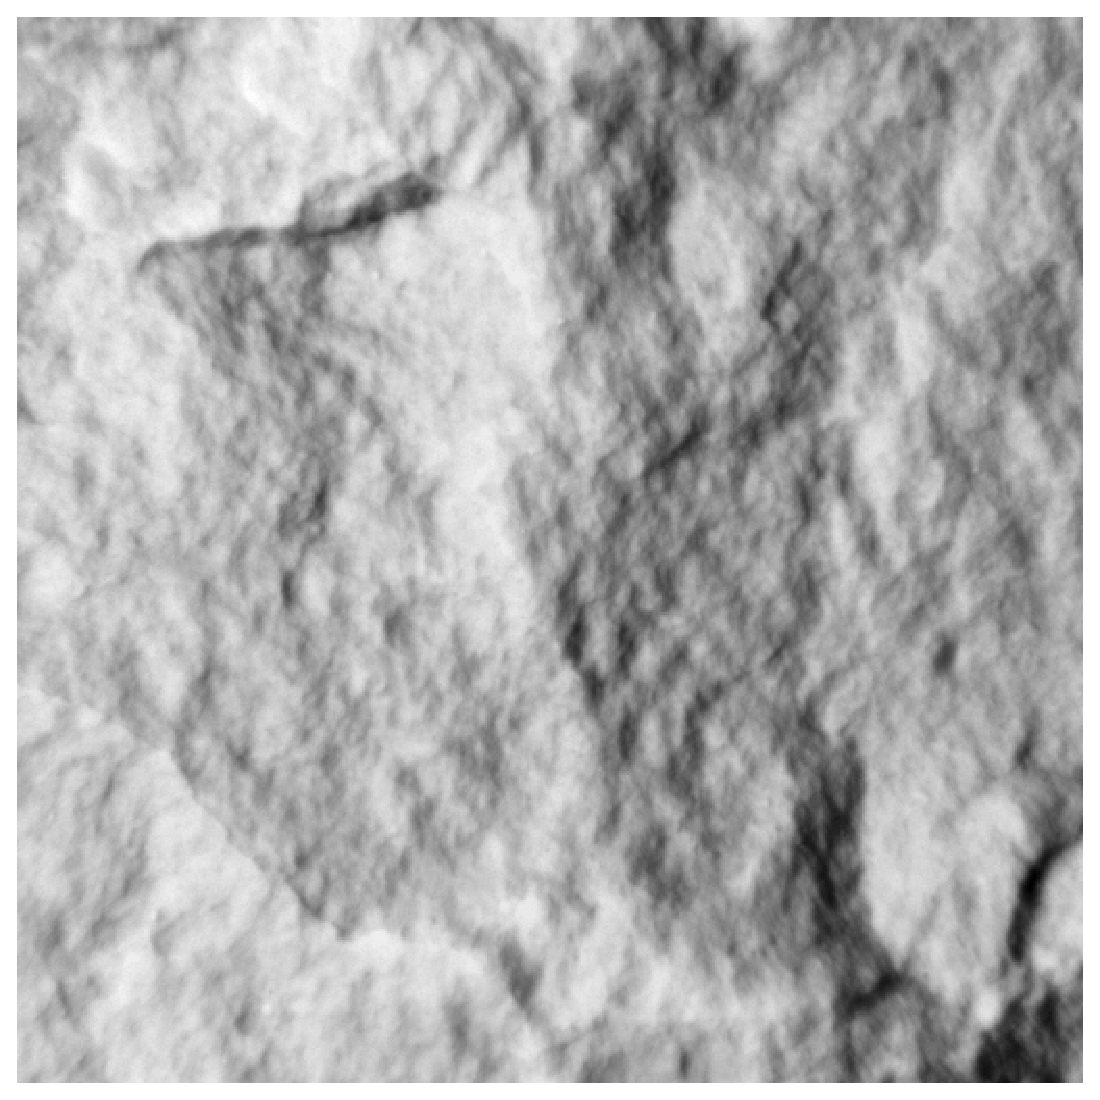
\epsfig{file=images/db/aaa.eps, width=0.15\linewidth}}
		\subfigure[aab]{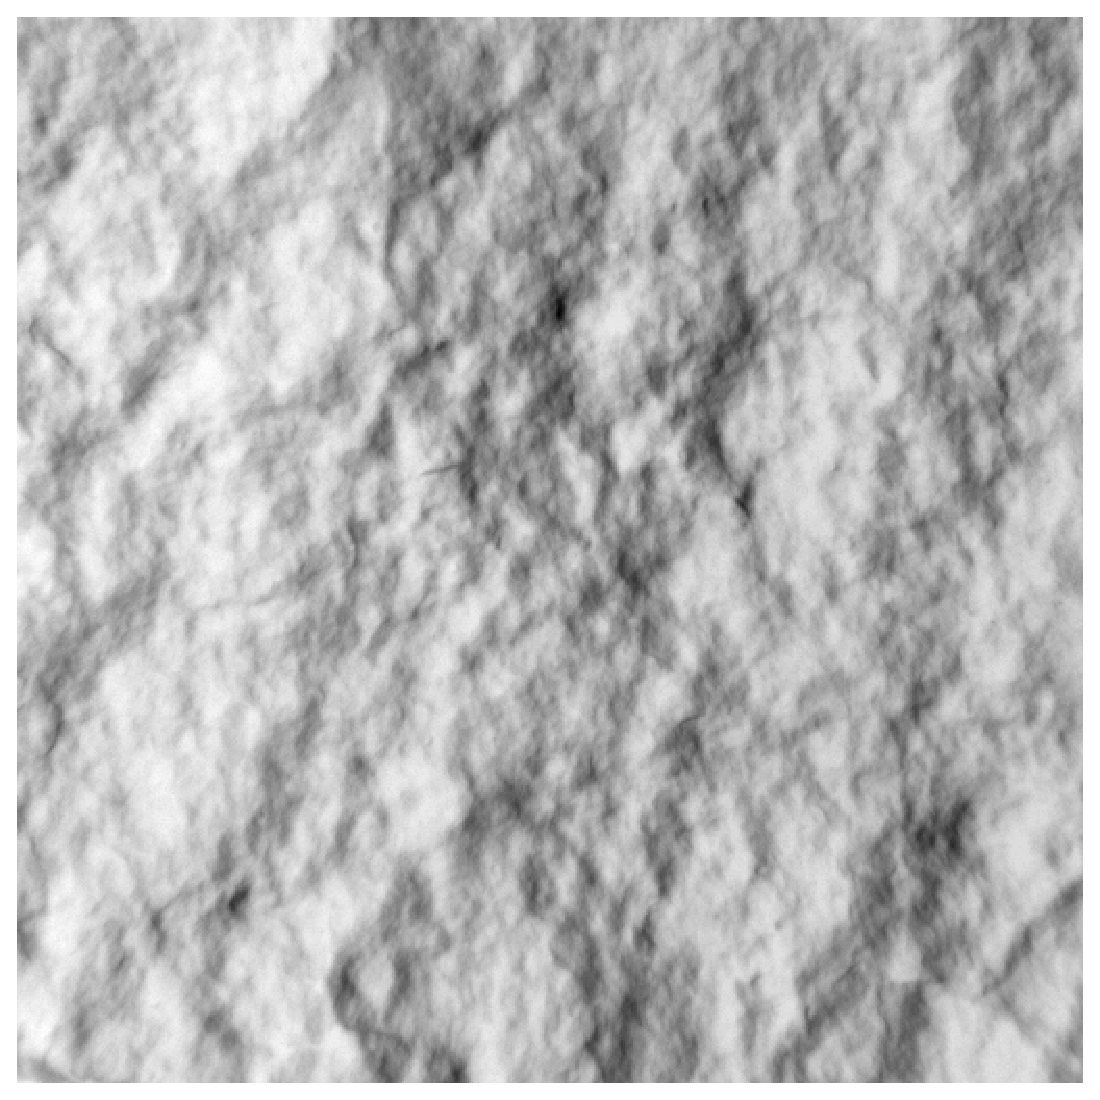
\epsfig{file=images/db/aab.eps, width=0.15\linewidth}}
		\subfigure[aaj]{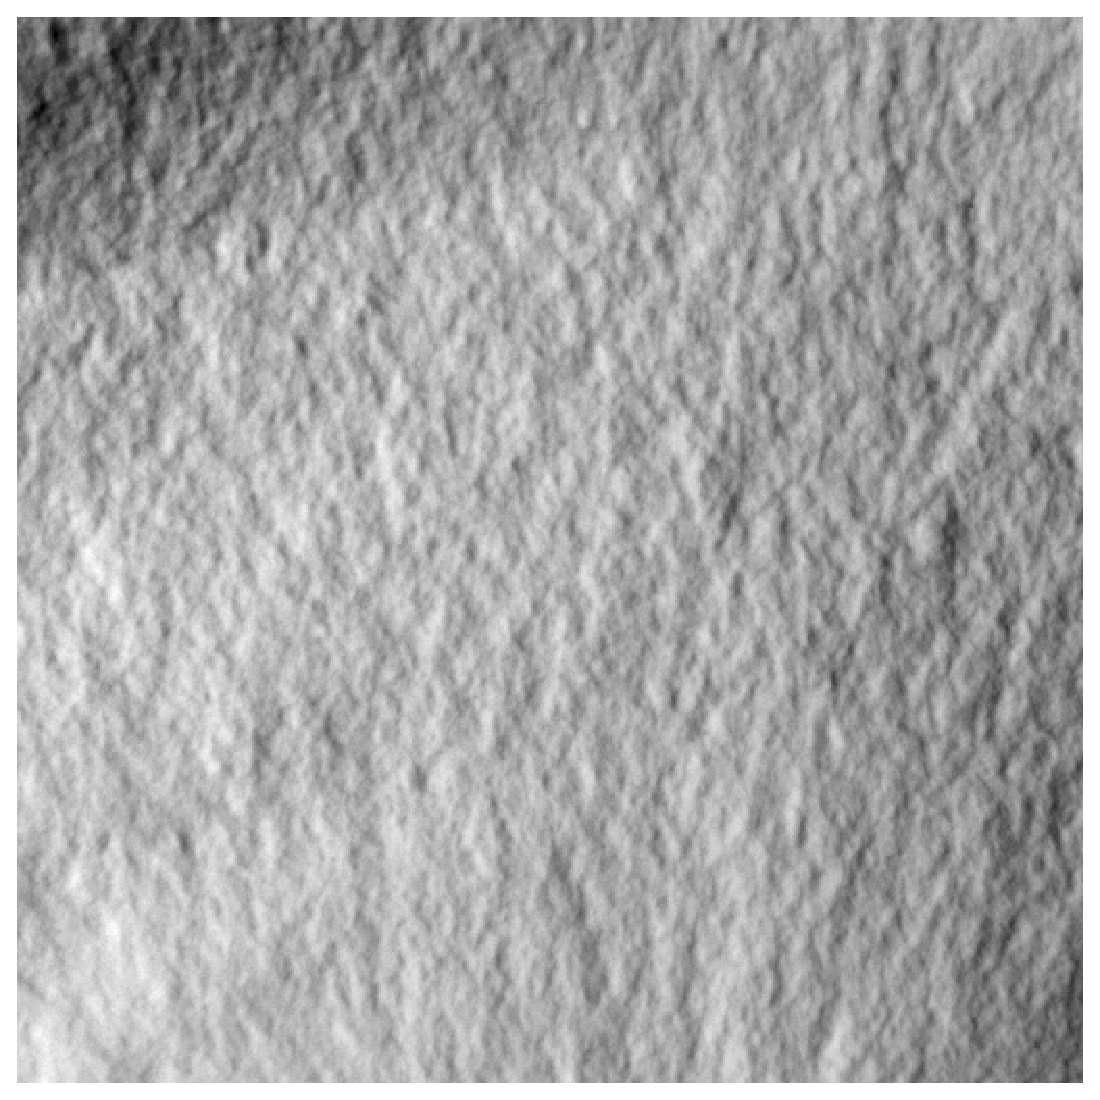
\epsfig{file=images/db/aaj.eps, width=0.15\linewidth}}
		\subfigure[aam]{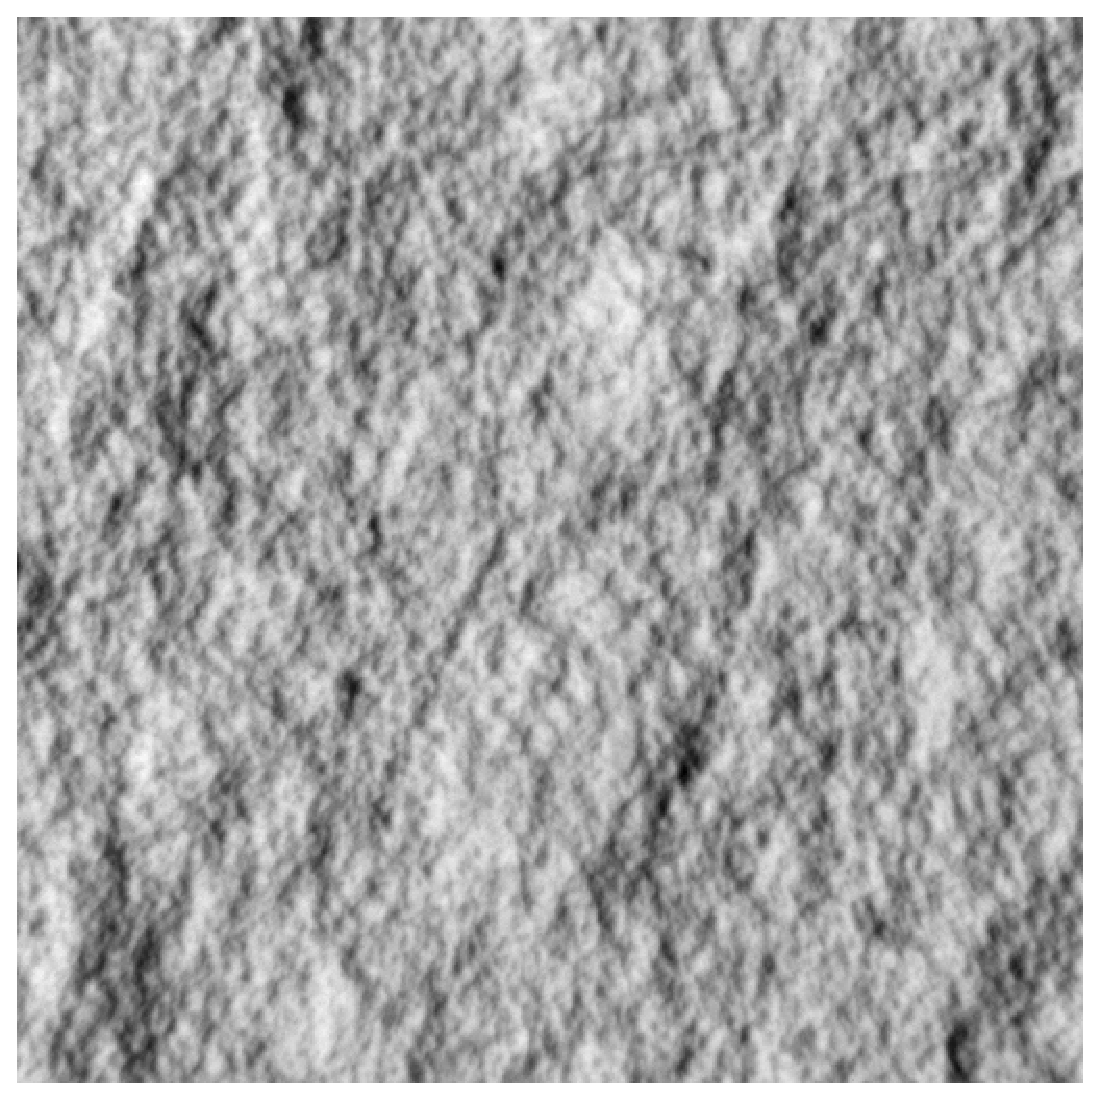
\epsfig{file=images/db/aam.eps, width=0.15\linewidth}}
		\subfigure[aan]{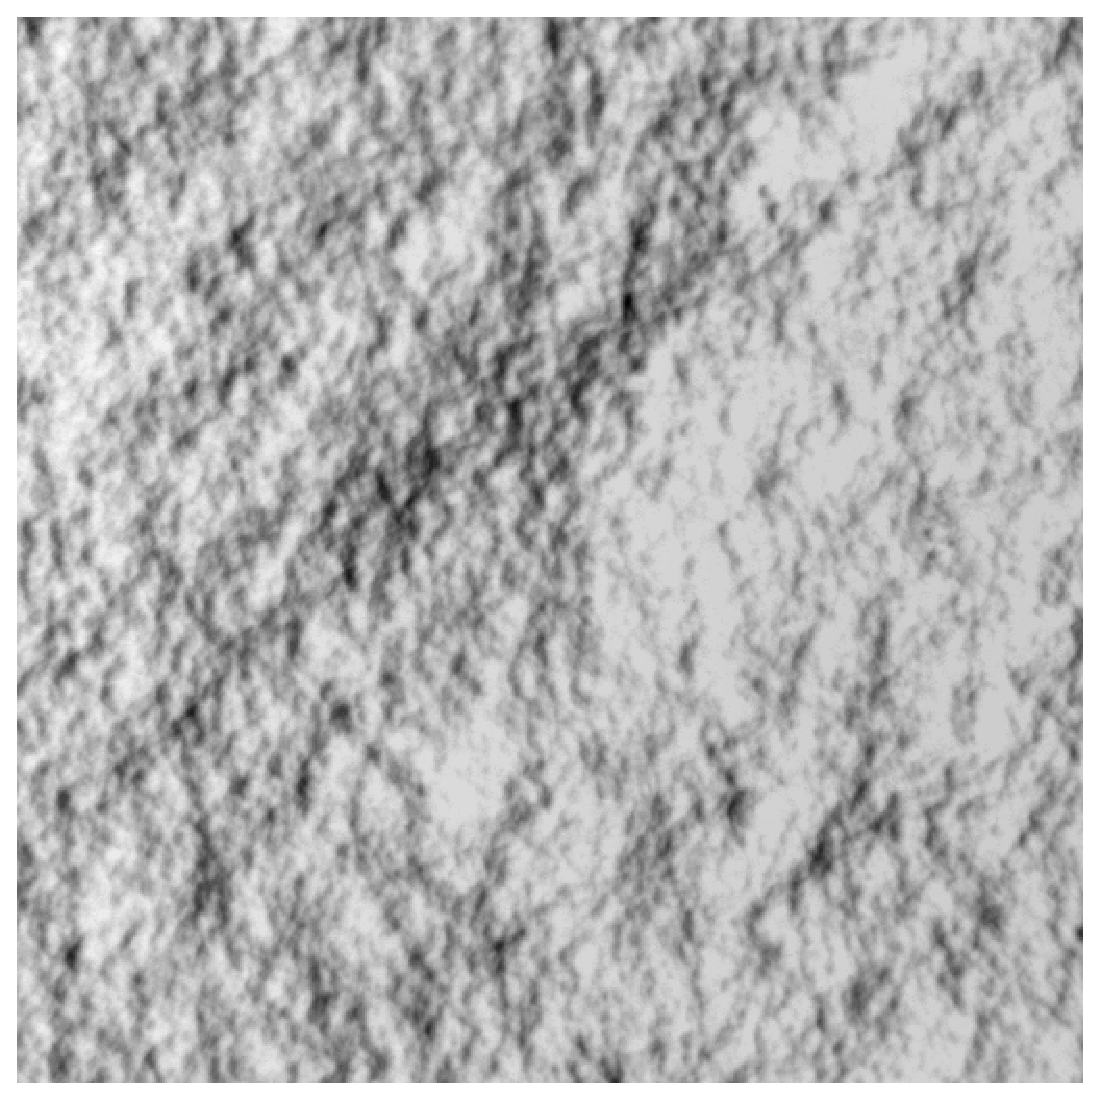
\epsfig{file=images/db/aan.eps, width=0.15\linewidth}}

		\subfigure[aao]{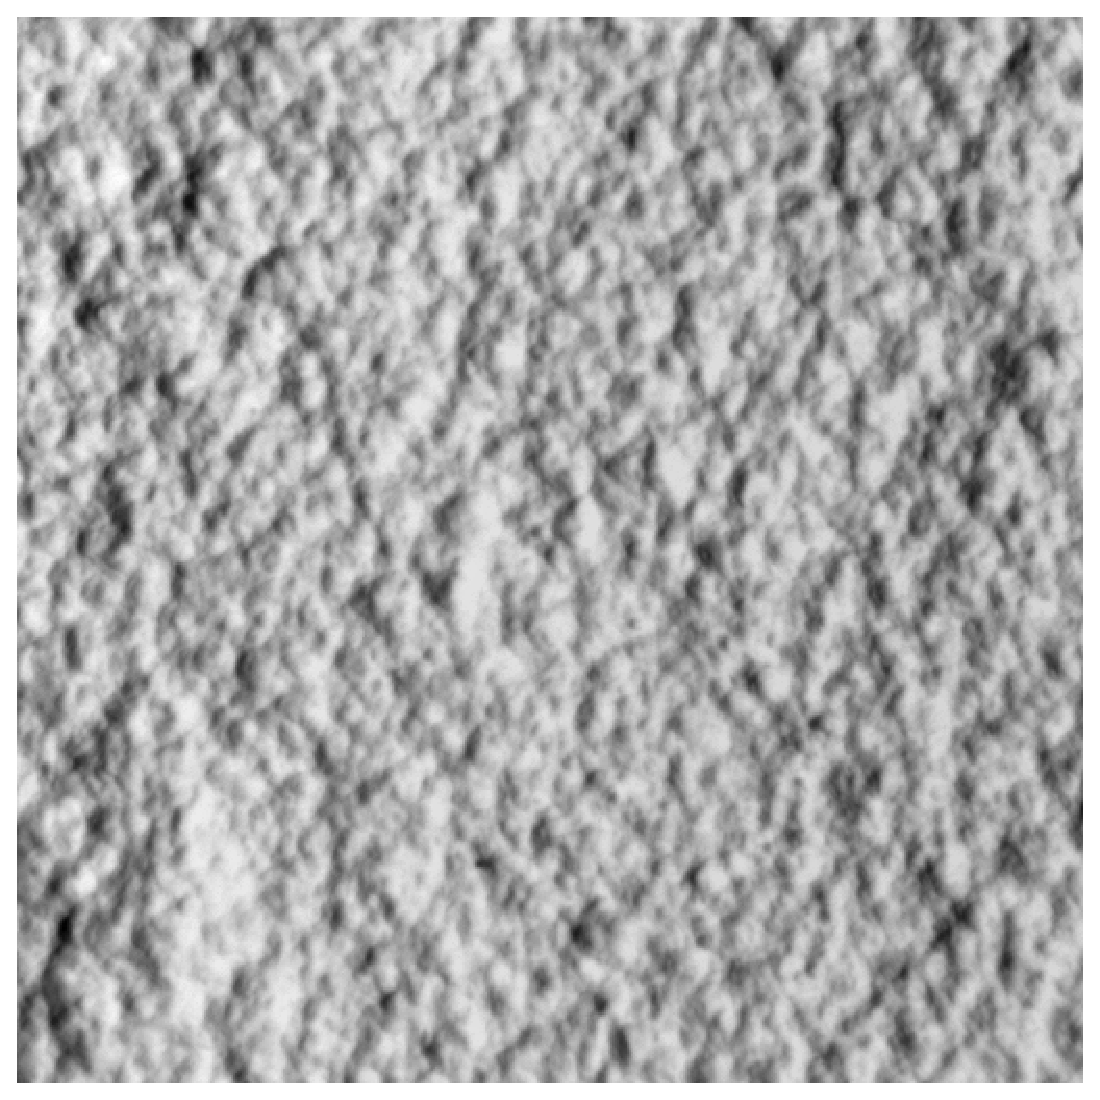
\epsfig{file=images/db/aao.eps, width=0.15\linewidth}}
		\subfigure[aar]{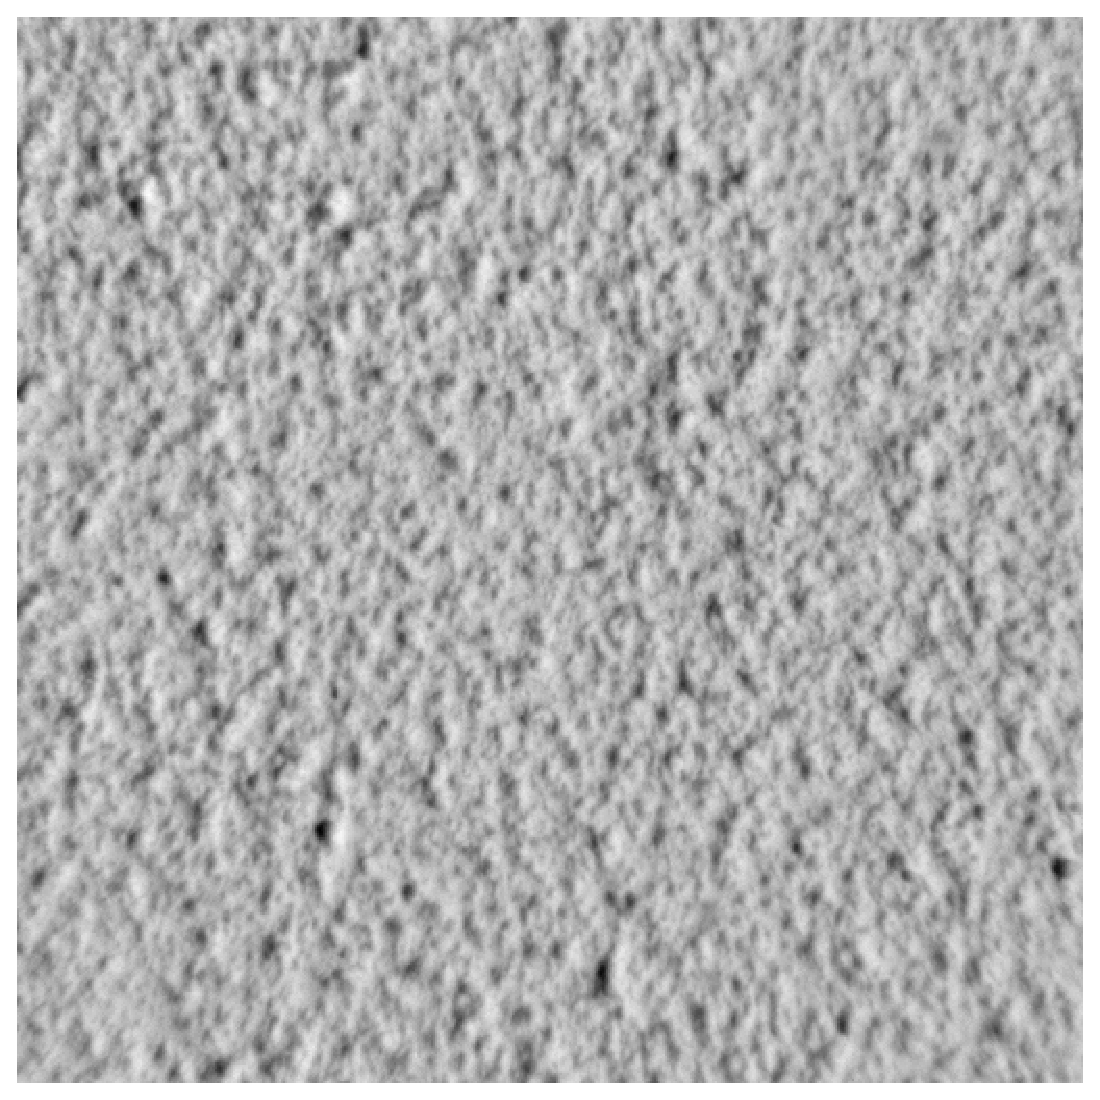
\epsfig{file=images/db/aar.eps, width=0.15\linewidth}}
		\subfigure[aas]{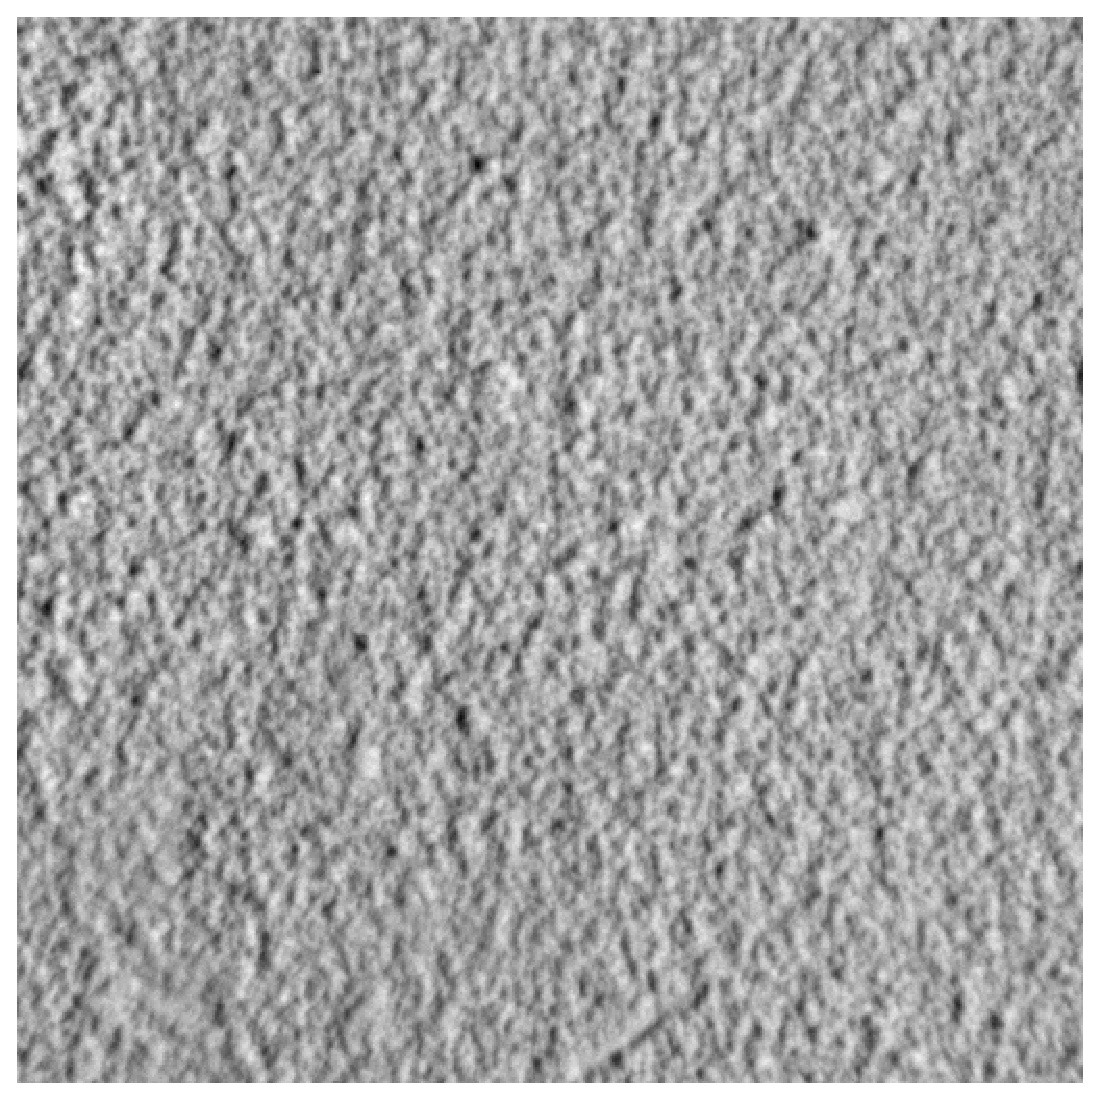
\epsfig{file=images/db/aas.eps, width=0.15\linewidth}}
		\subfigure[aba]{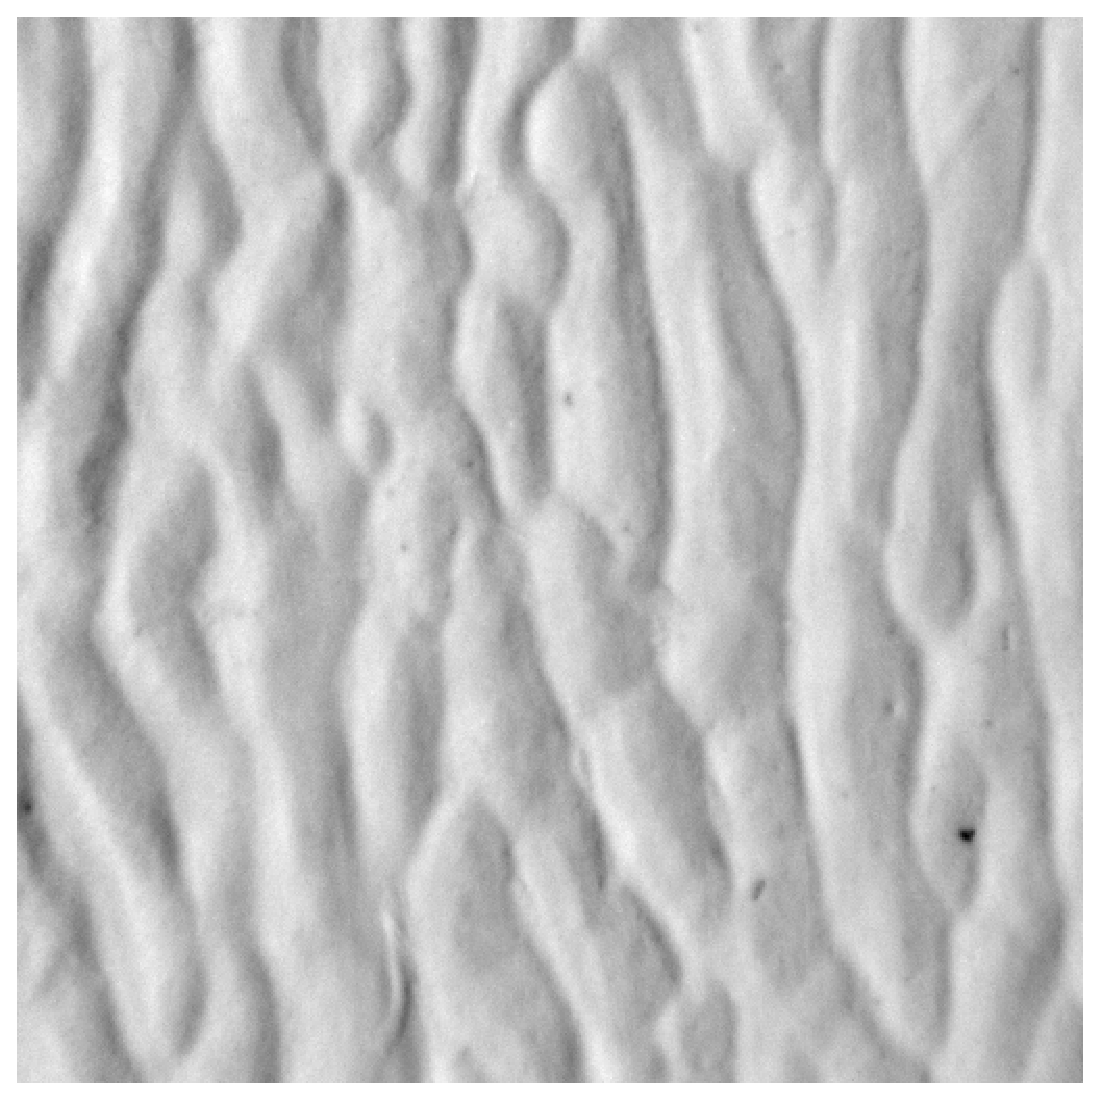
\epsfig{file=images/db/aba.eps, width=0.15\linewidth}}
		\subfigure[abj]{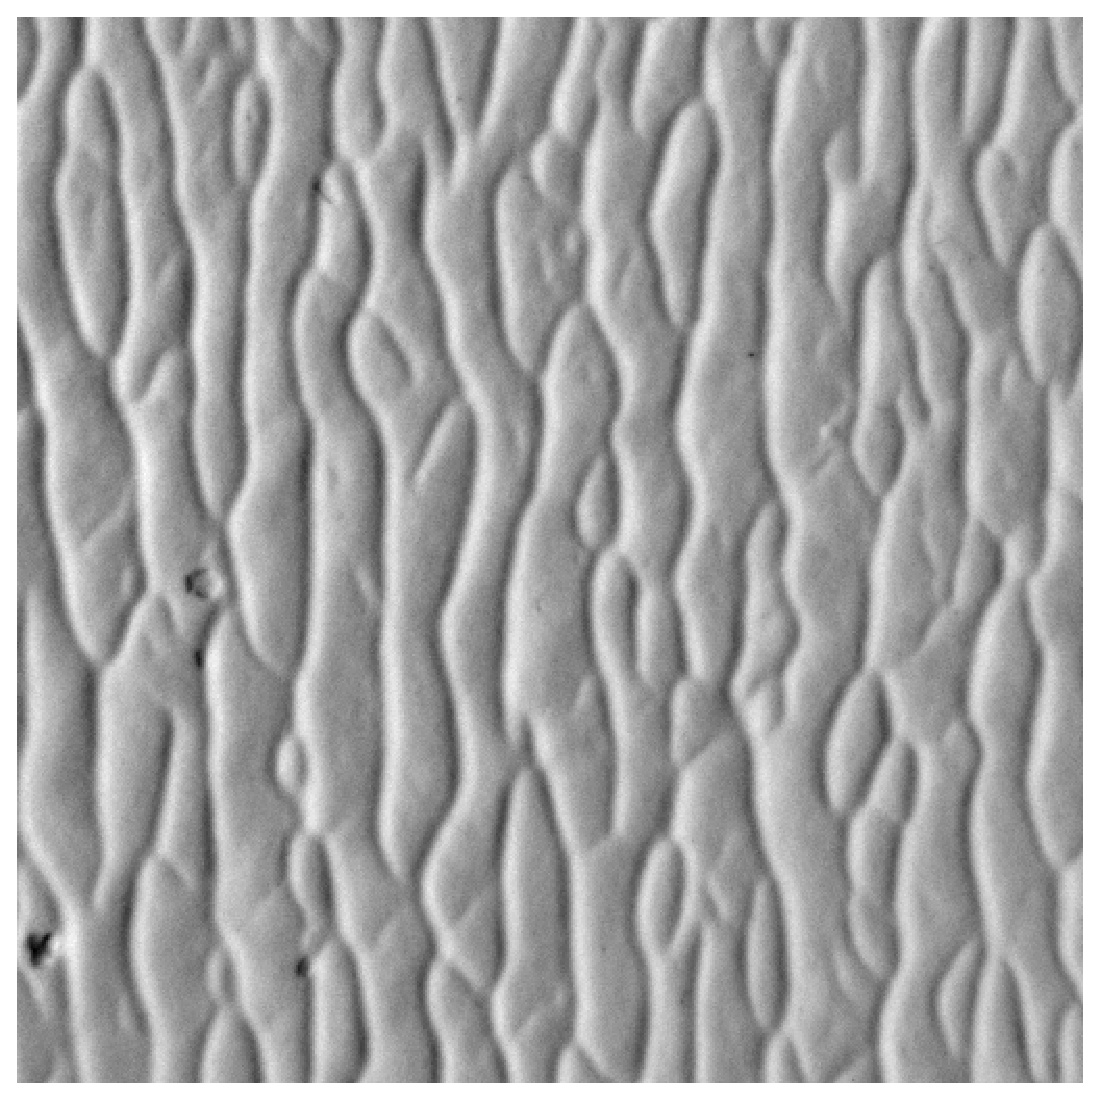
\epsfig{file=images/db/abj.eps, width=0.15\linewidth}}

		\subfigure[abk]{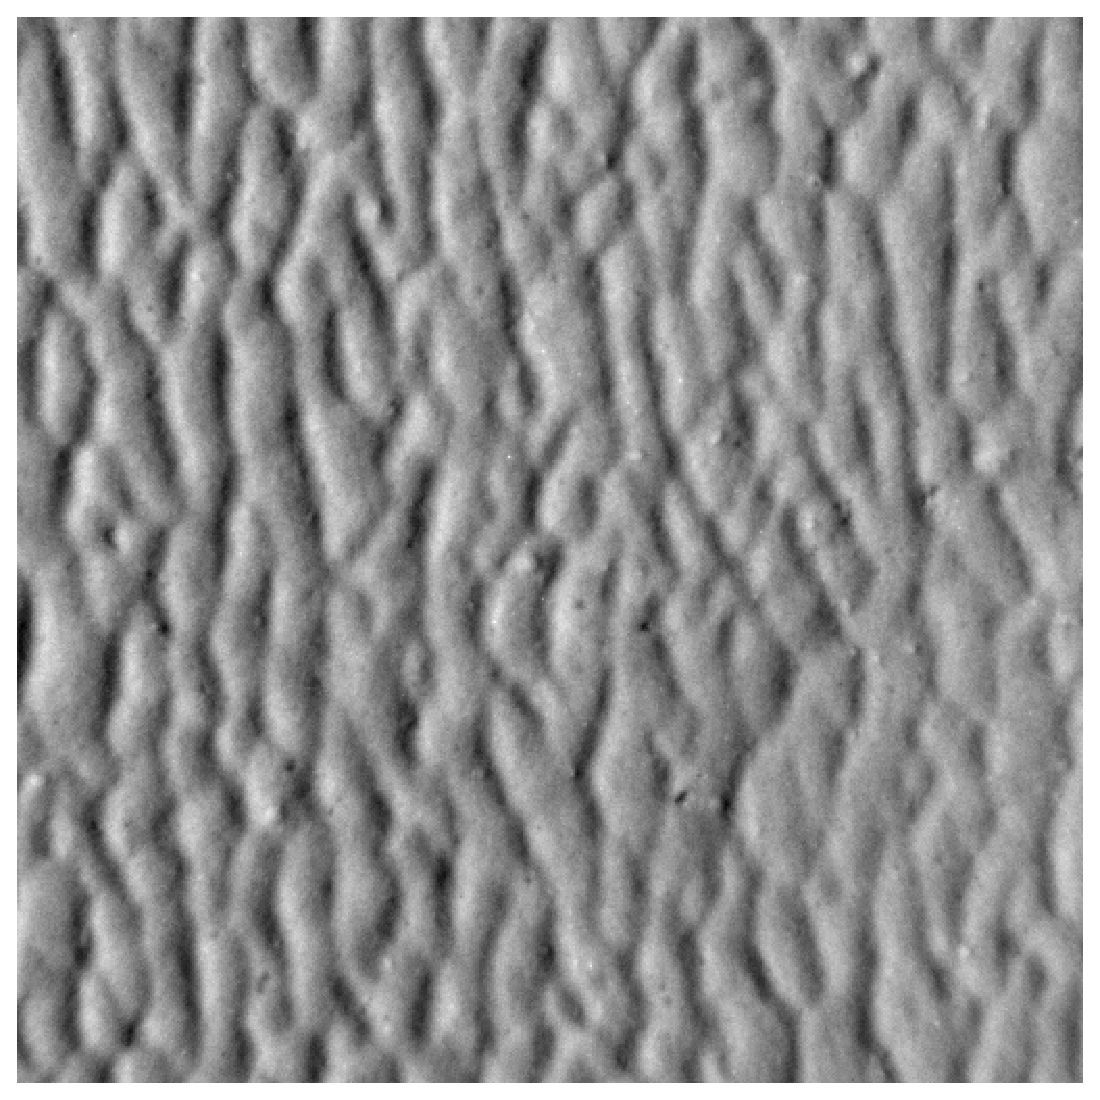
\epsfig{file=images/db/abk.eps, width=0.15\linewidth}}
		\subfigure[acc]{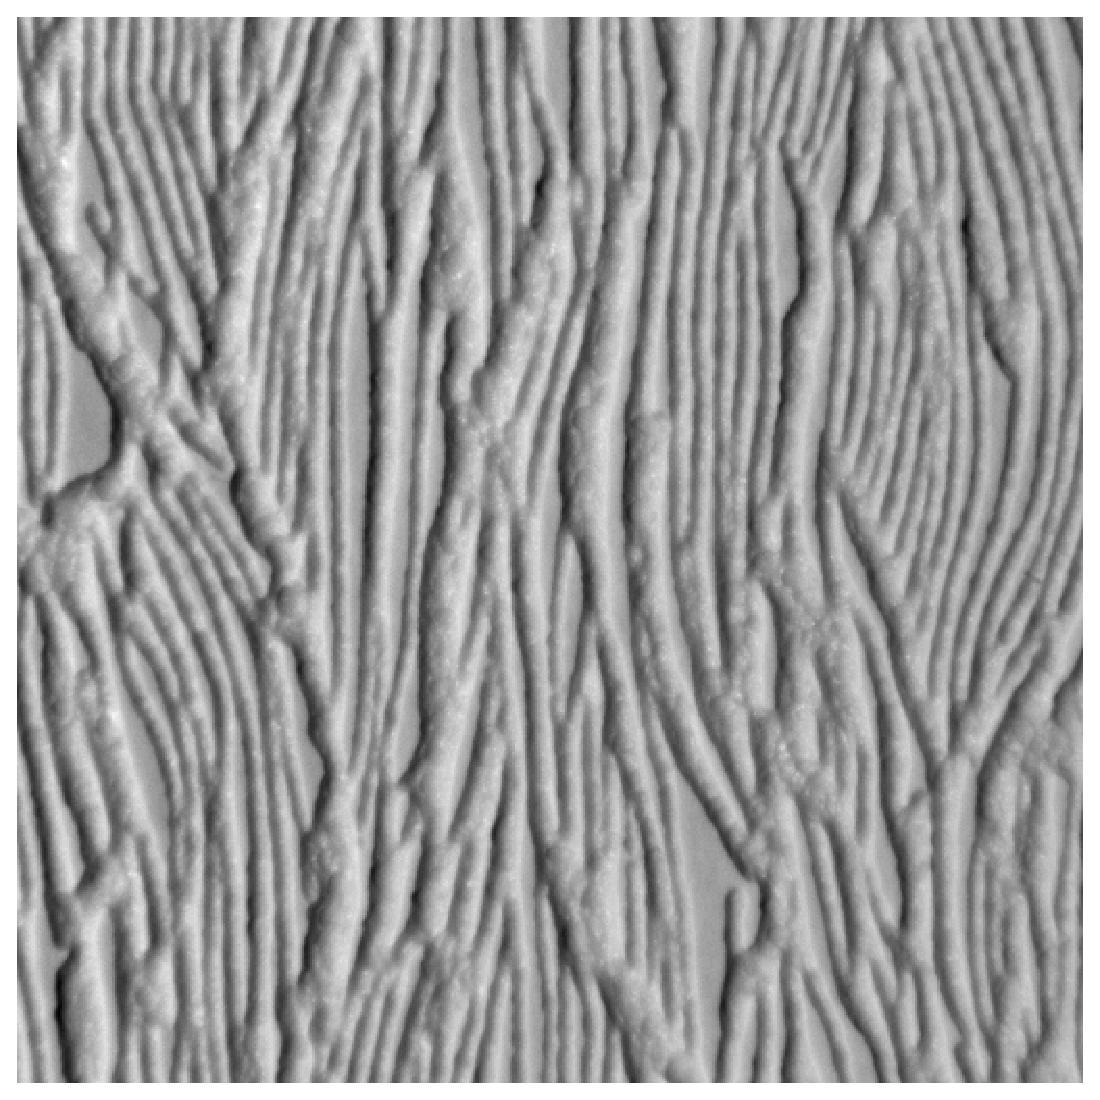
\epsfig{file=images/db/acc.eps, width=0.15\linewidth}}
		\subfigure[acd]{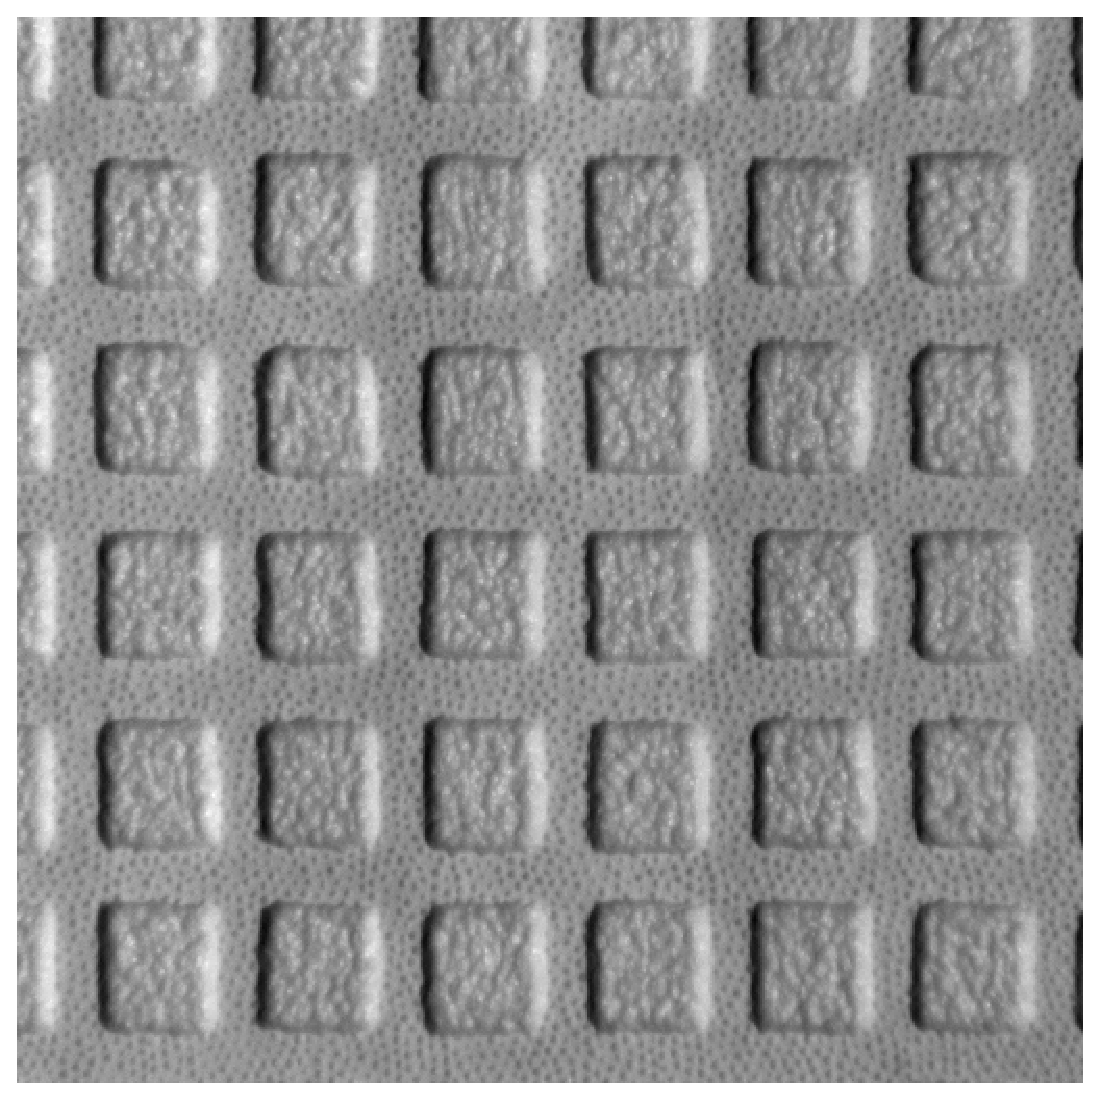
\epsfig{file=images/db/acd.eps, width=0.15\linewidth}}
		\subfigure[ace]{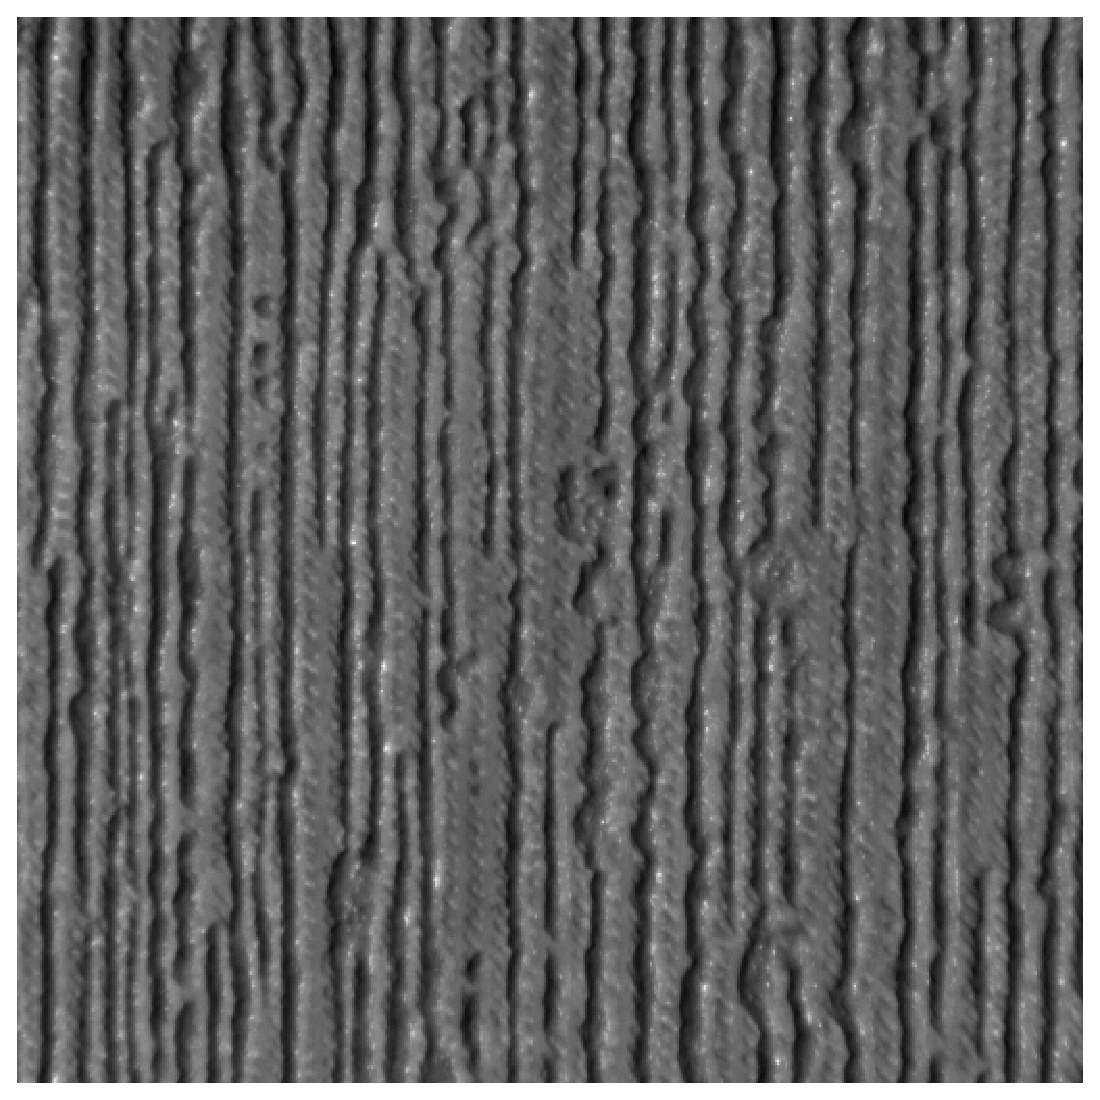
\epsfig{file=images/db/ace.eps, width=0.15\linewidth}}
		\subfigure[adb]{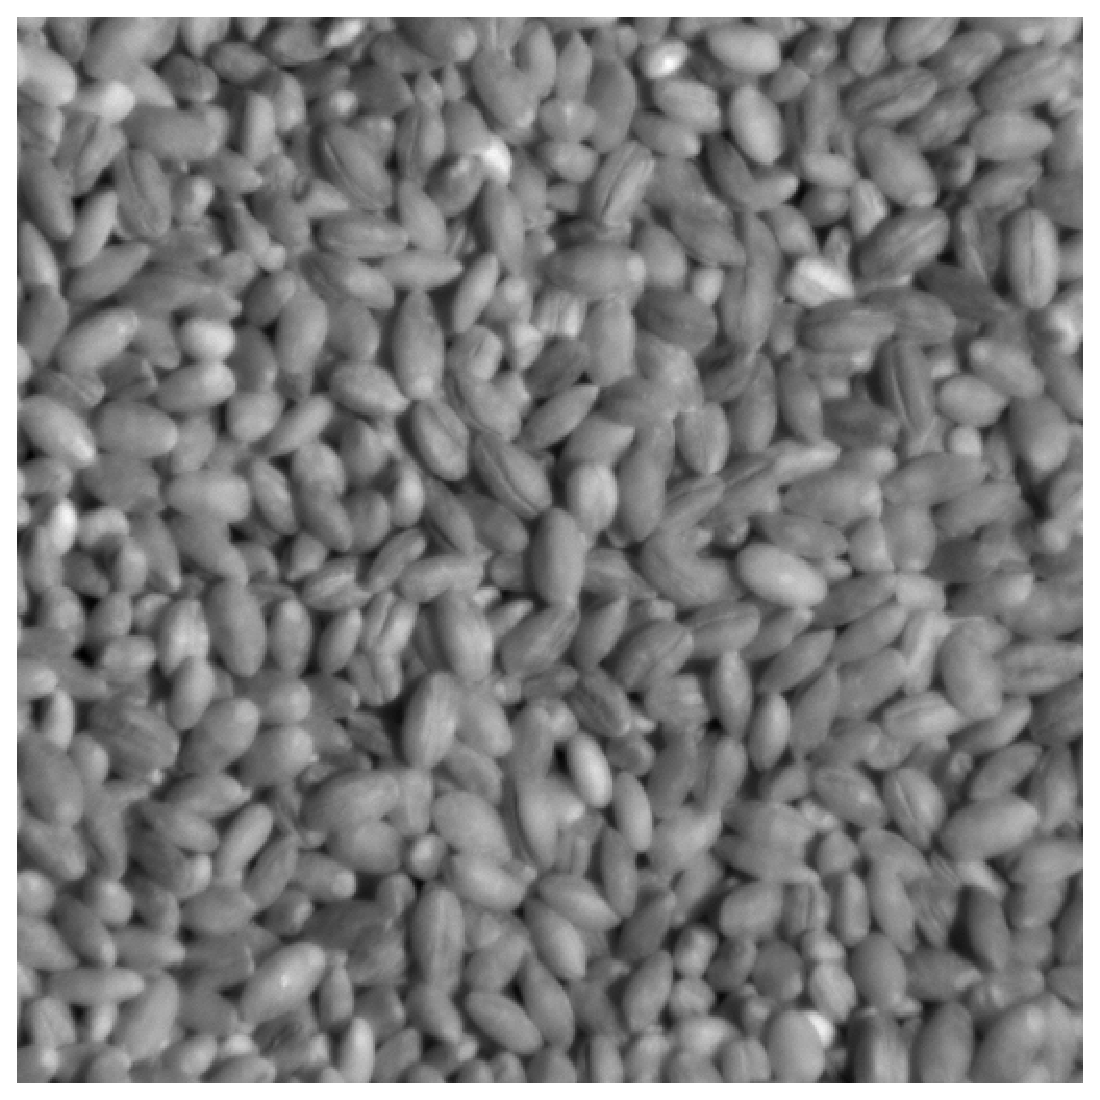
\epsfig{file=images/db/adb.eps, width=0.15\linewidth}}

		\subfigure[adc]{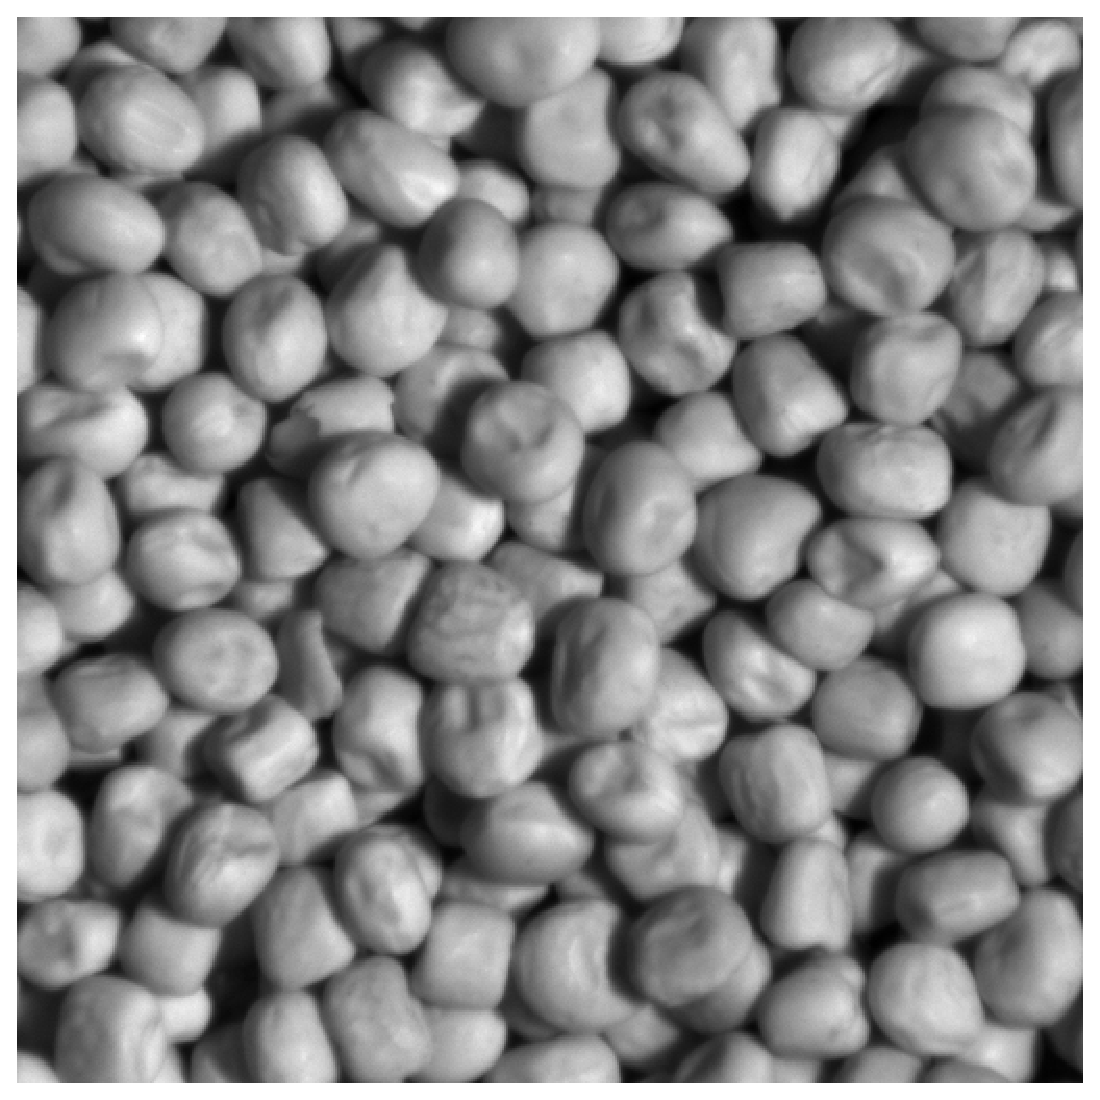
\epsfig{file=images/db/adc.eps, width=0.15\linewidth}}
		\subfigure[add]{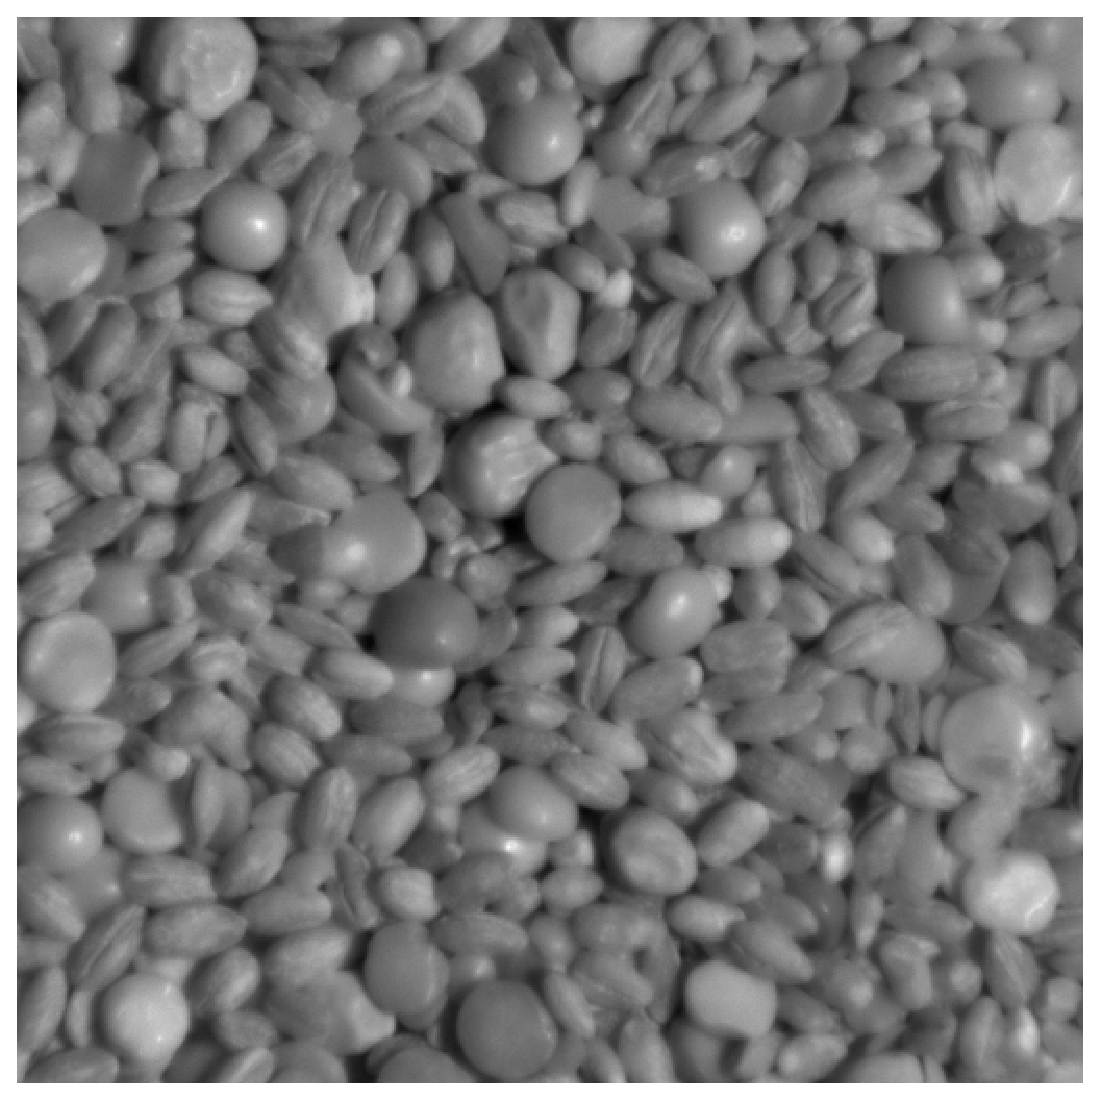
\epsfig{file=images/db/add.eps, width=0.15\linewidth}}
		\subfigure[ade]{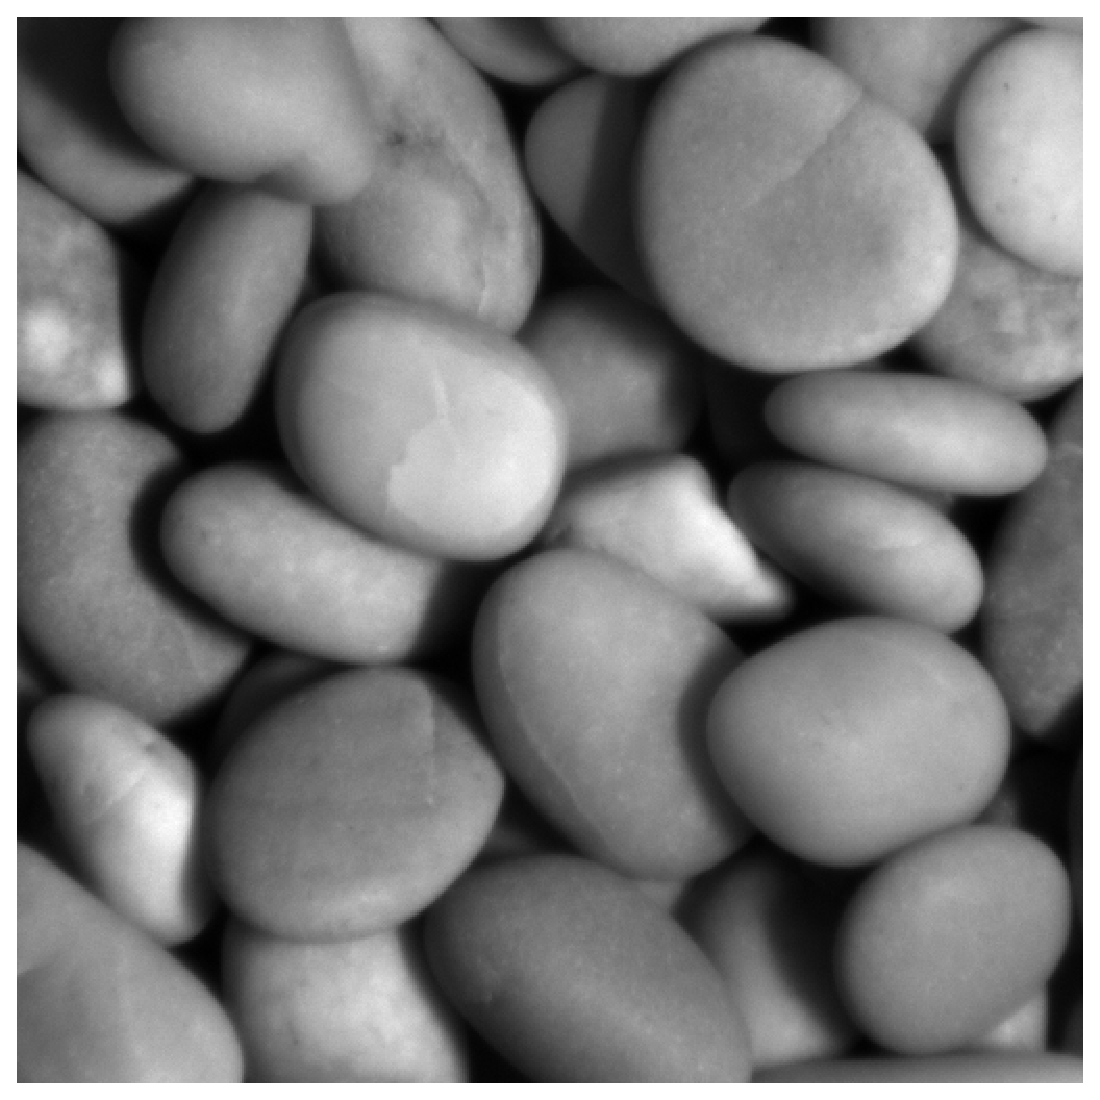
\epsfig{file=images/db/ade.eps, width=0.15\linewidth}}
		\subfigure[adg]{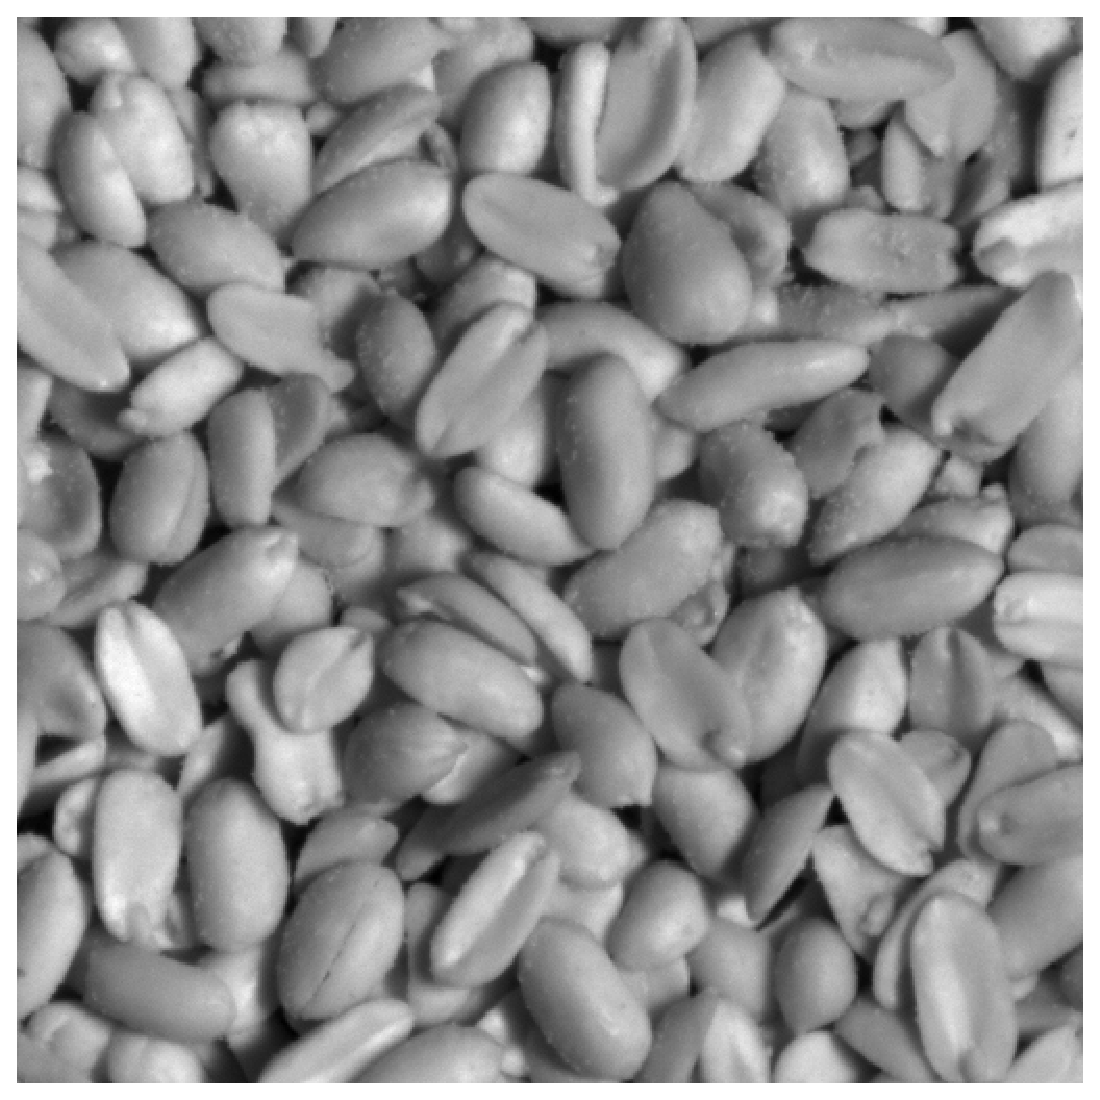
\epsfig{file=images/db/adg.eps, width=0.15\linewidth}}
		\subfigure[adh]{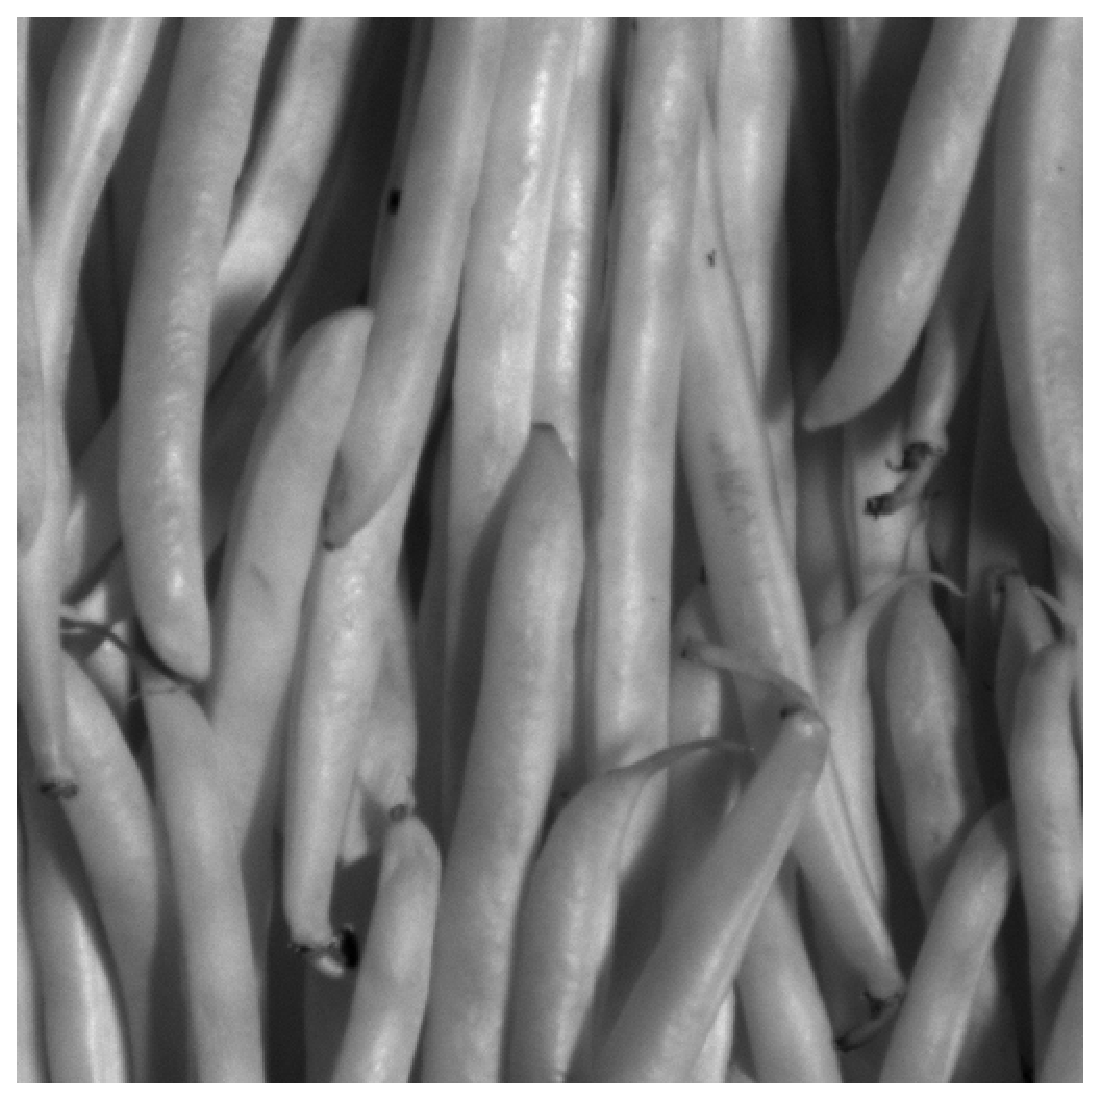
\epsfig{file=images/db/adh.eps, width=0.15\linewidth}}
	\end{center}
	\caption{{\it The material classes taken from the PhoTex database. The example images are registered under a slant of $30^0$ and a tilt of $0^0$.}}
	\label{fig:PhoTexData}
\end{figure}
%\end{comment}

\subsection{Shiny material classes}
Because three out of five reflection models simulate specularity only, the previous dataset might not be good enough to measure improvements made by these reflection models. For this reason, a new dataset is selected from the {\it PhoTex} database with more specular properties. 

The material classes selected are shown in figure \ref{fig:PhoTexData2}. This dataset consists of 10 material classes, recorded under a slant of $75^0$ and tilts of $0^0$ to $350^0$ in increments of $10^0$, giving a total of 36 images for each material class. The material classes are shown in figure \ref{fig:PhoTexData2}.

%\begin{comment}
\begin{figure}[h]
	\begin{center}
		\subfigure[aaa]{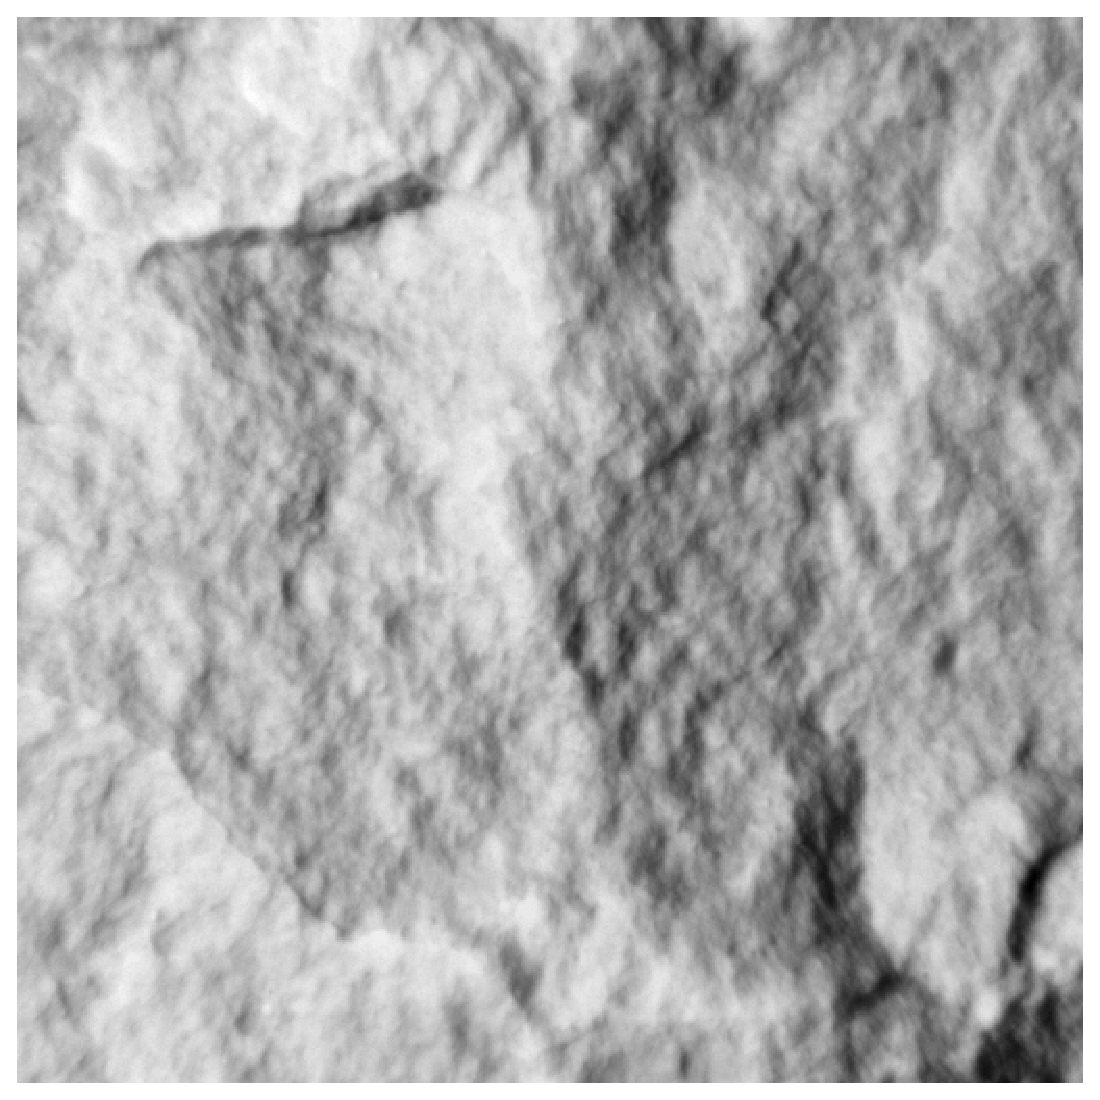
\epsfig{file=images/db/aaa.eps, width=0.15\linewidth}}
		\subfigure[aab]{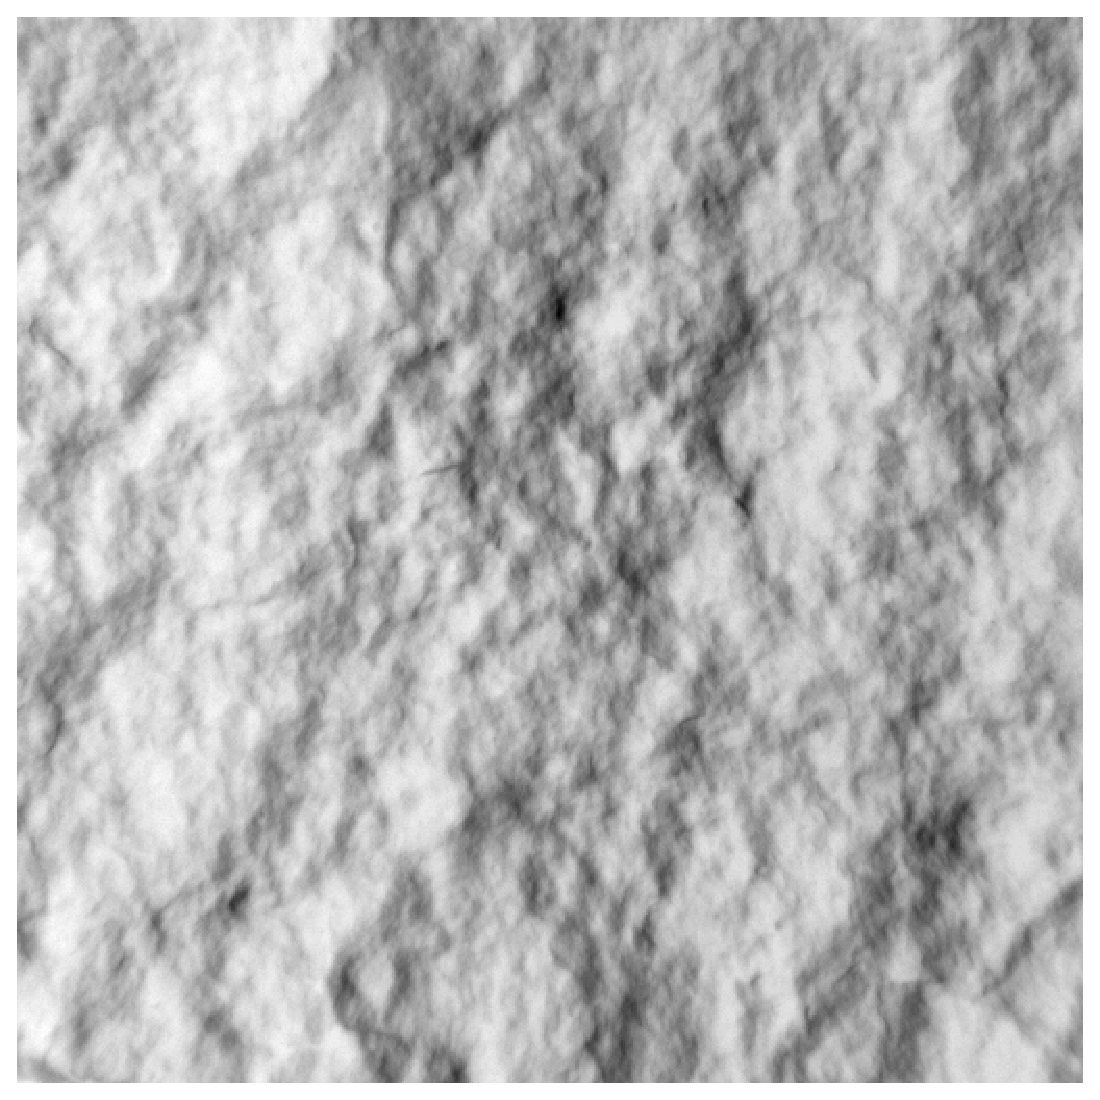
\epsfig{file=images/db/aab.eps, width=0.15\linewidth}}
		\subfigure[aaj]{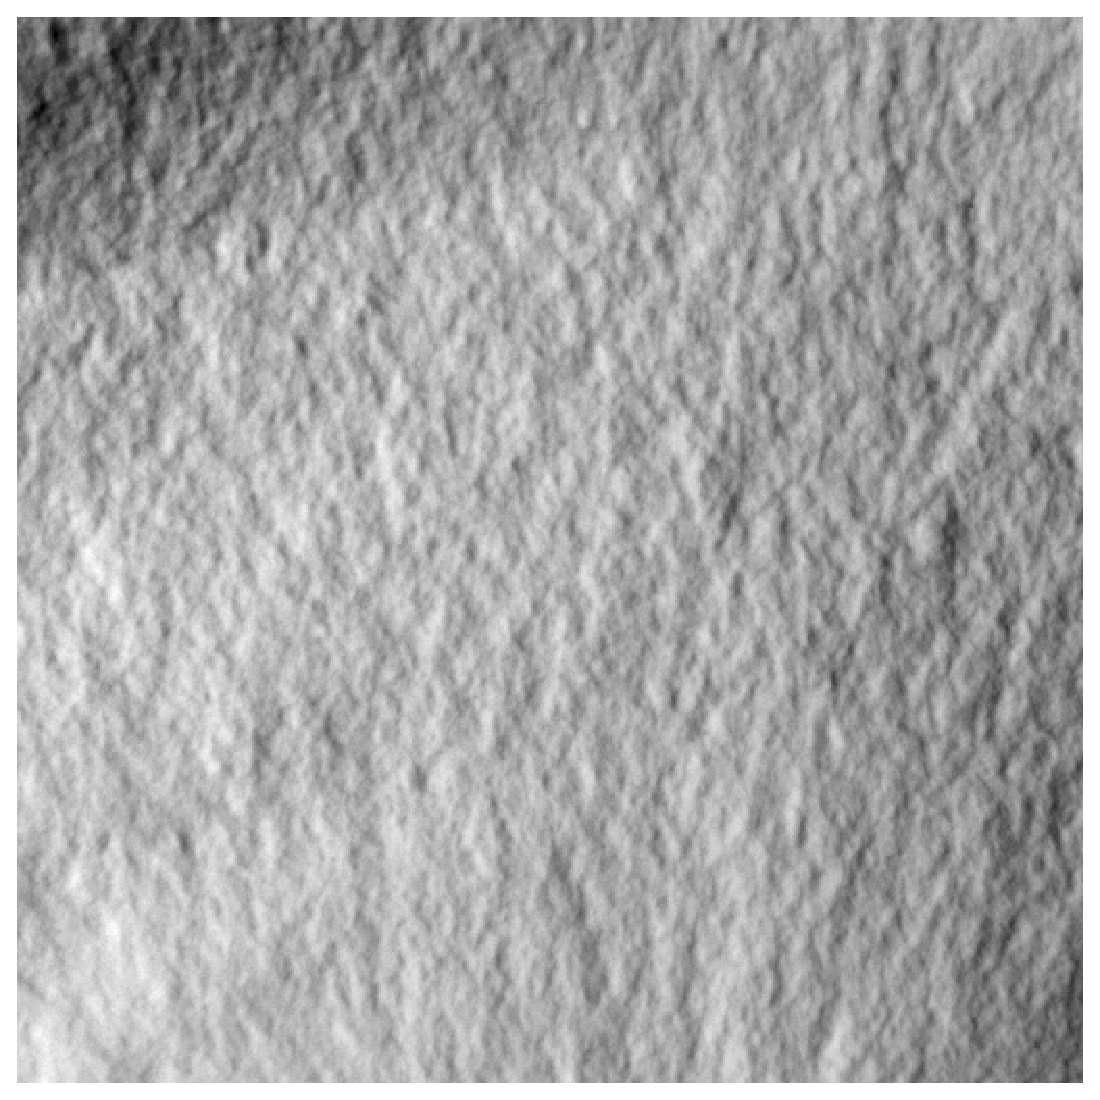
\epsfig{file=images/db/aaj.eps, width=0.15\linewidth}}
		\subfigure[aam]{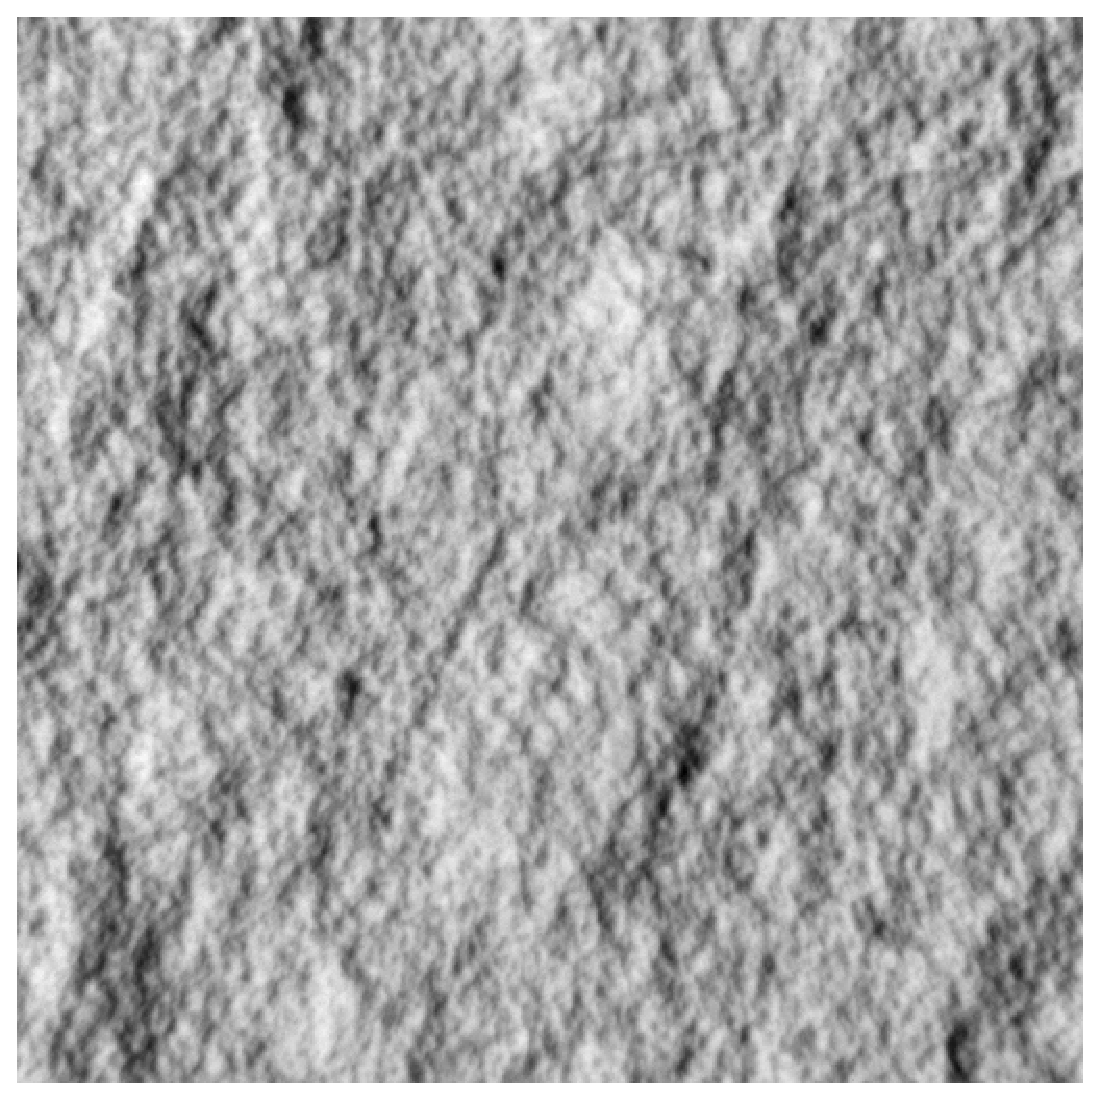
\epsfig{file=images/db/aam.eps, width=0.15\linewidth}}
		\subfigure[aan]{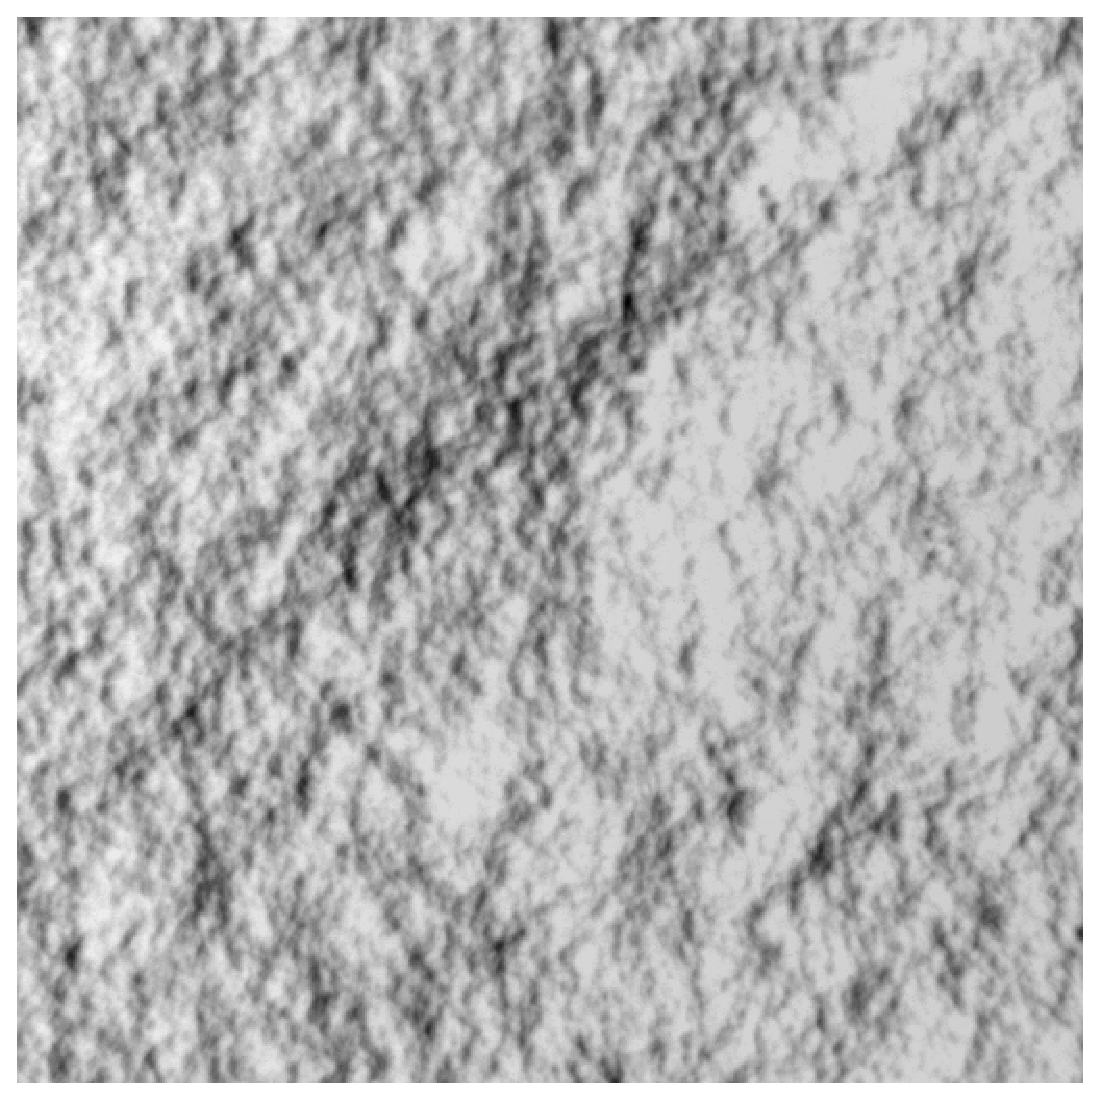
\epsfig{file=images/db/aan.eps, width=0.15\linewidth}}

		\subfigure[aao]{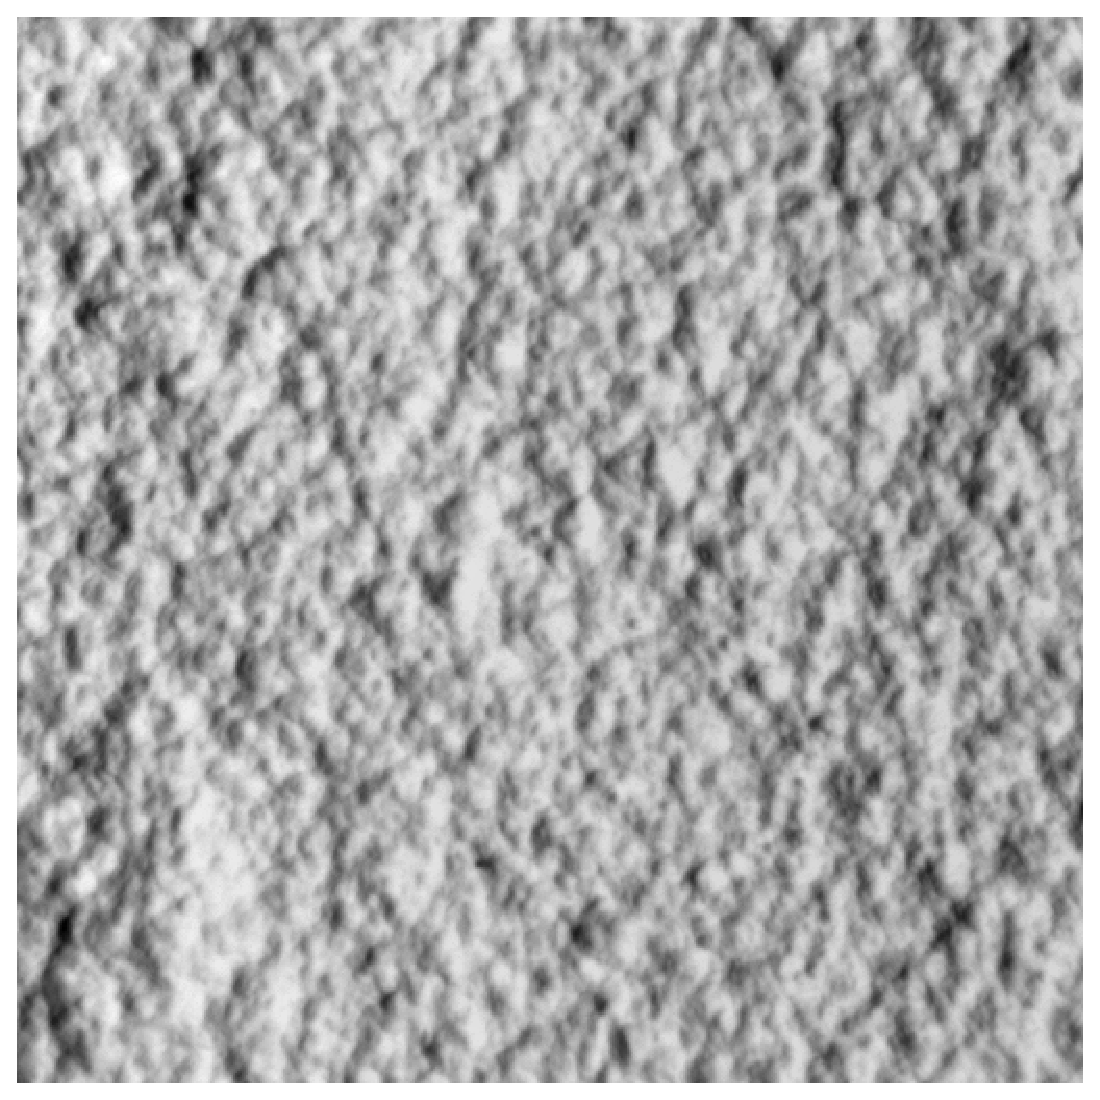
\epsfig{file=images/db/aao.eps, width=0.15\linewidth}}
		\subfigure[aar]{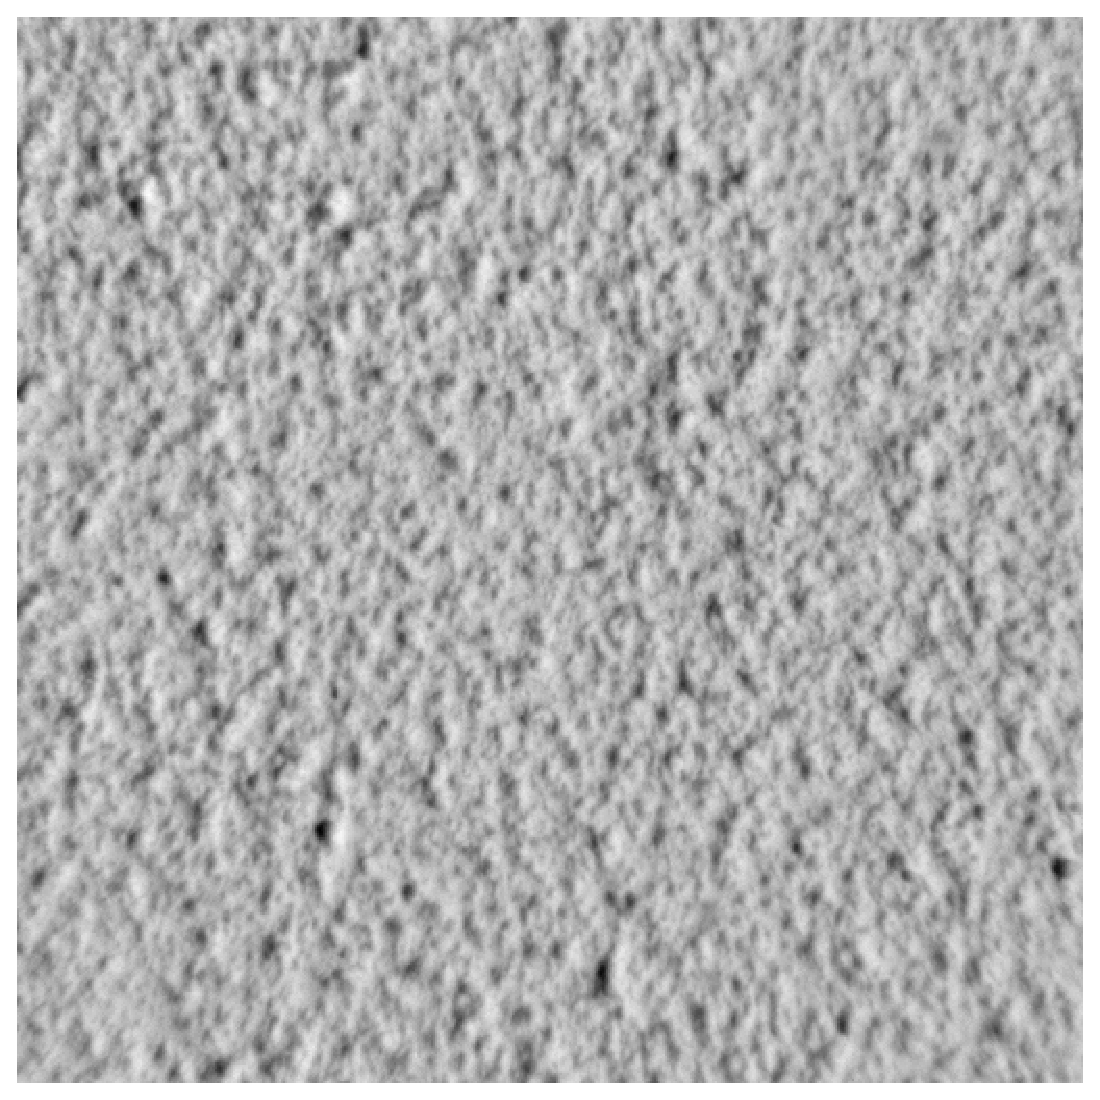
\epsfig{file=images/db/aar.eps, width=0.15\linewidth}}
		\subfigure[aas]{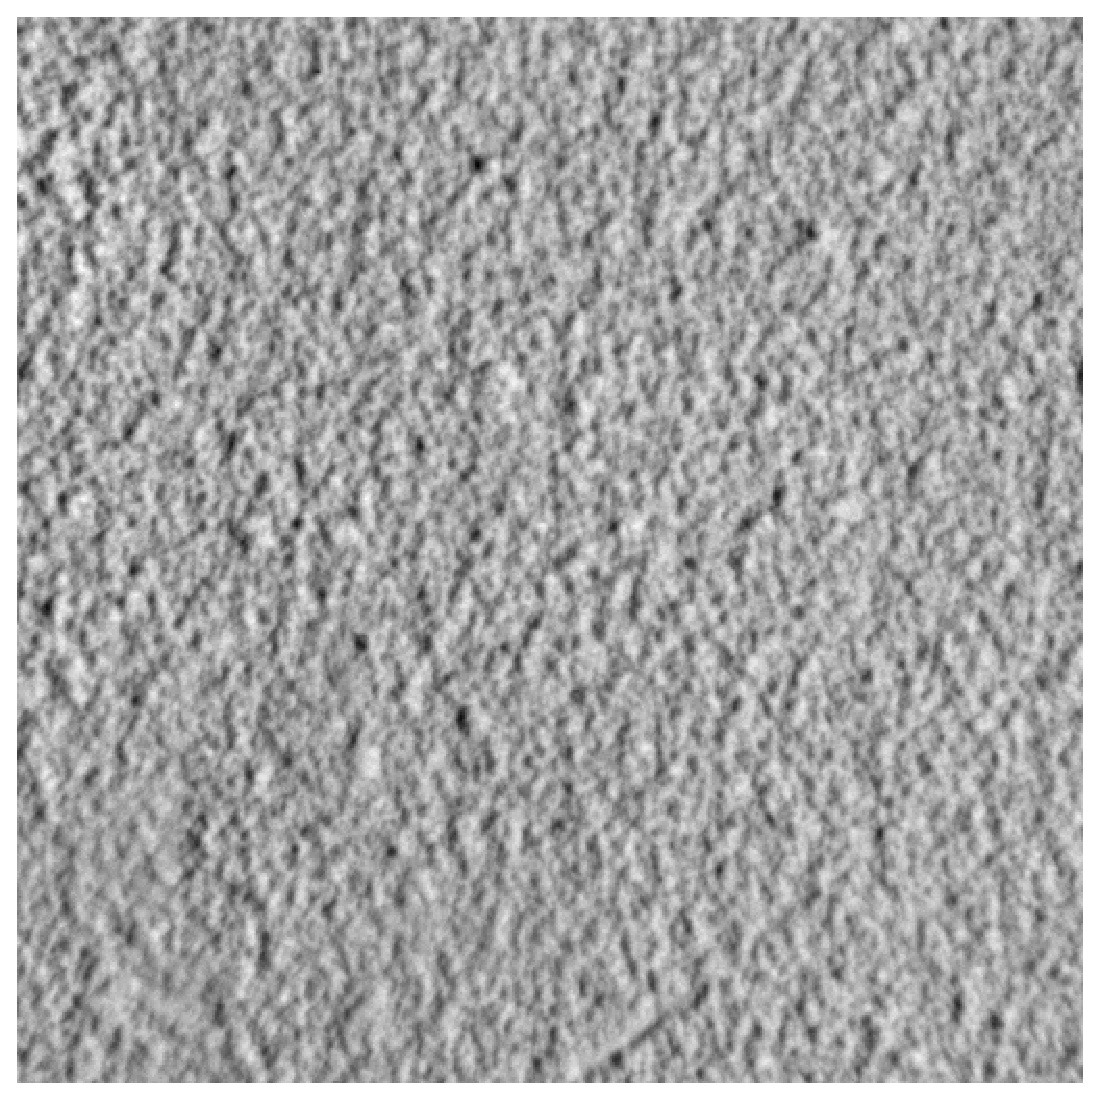
\epsfig{file=images/db/aas.eps, width=0.15\linewidth}}
		\subfigure[aba]{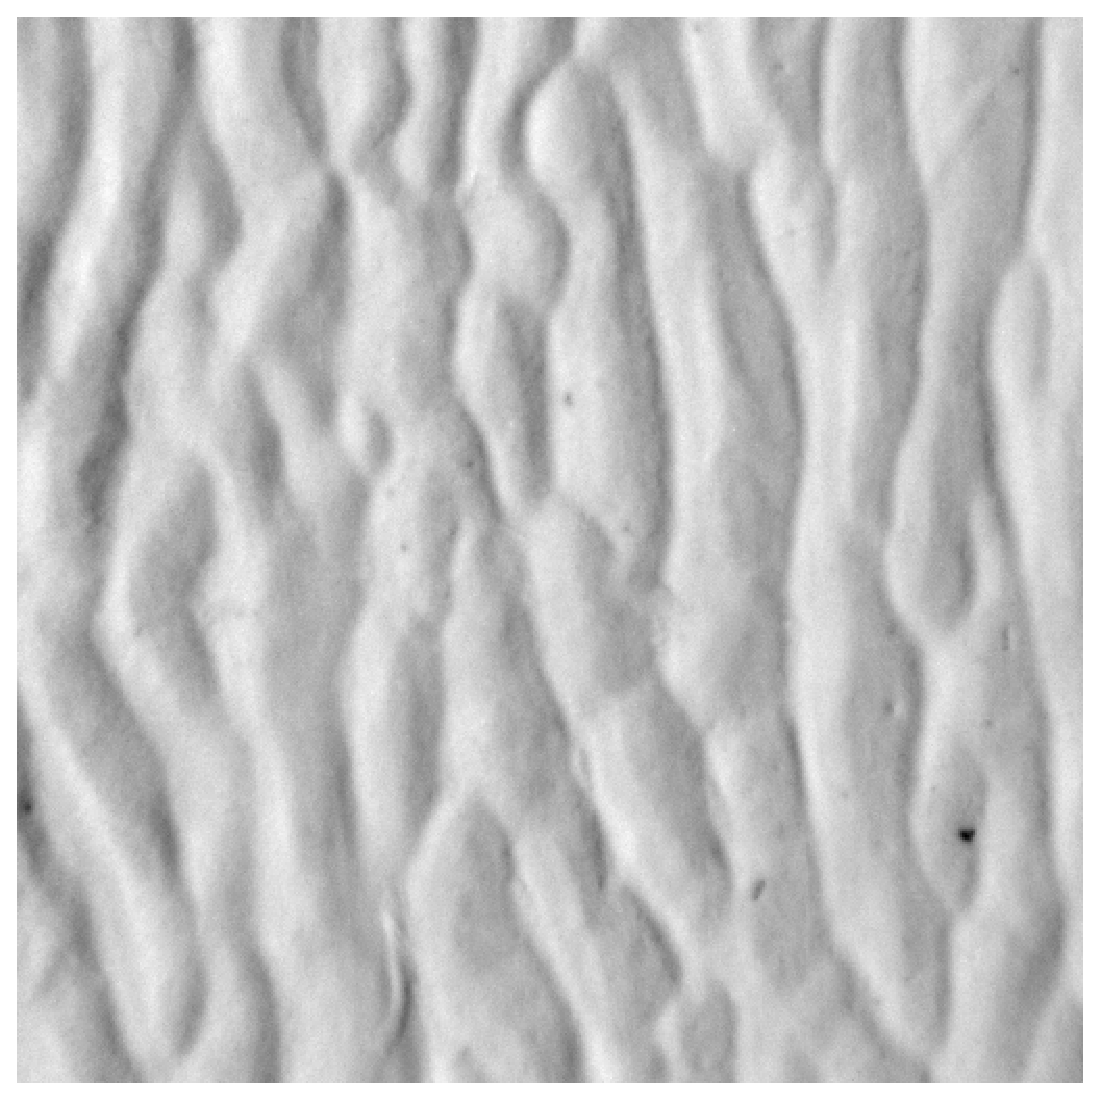
\epsfig{file=images/db/aba.eps, width=0.15\linewidth}}
		\subfigure[abj]{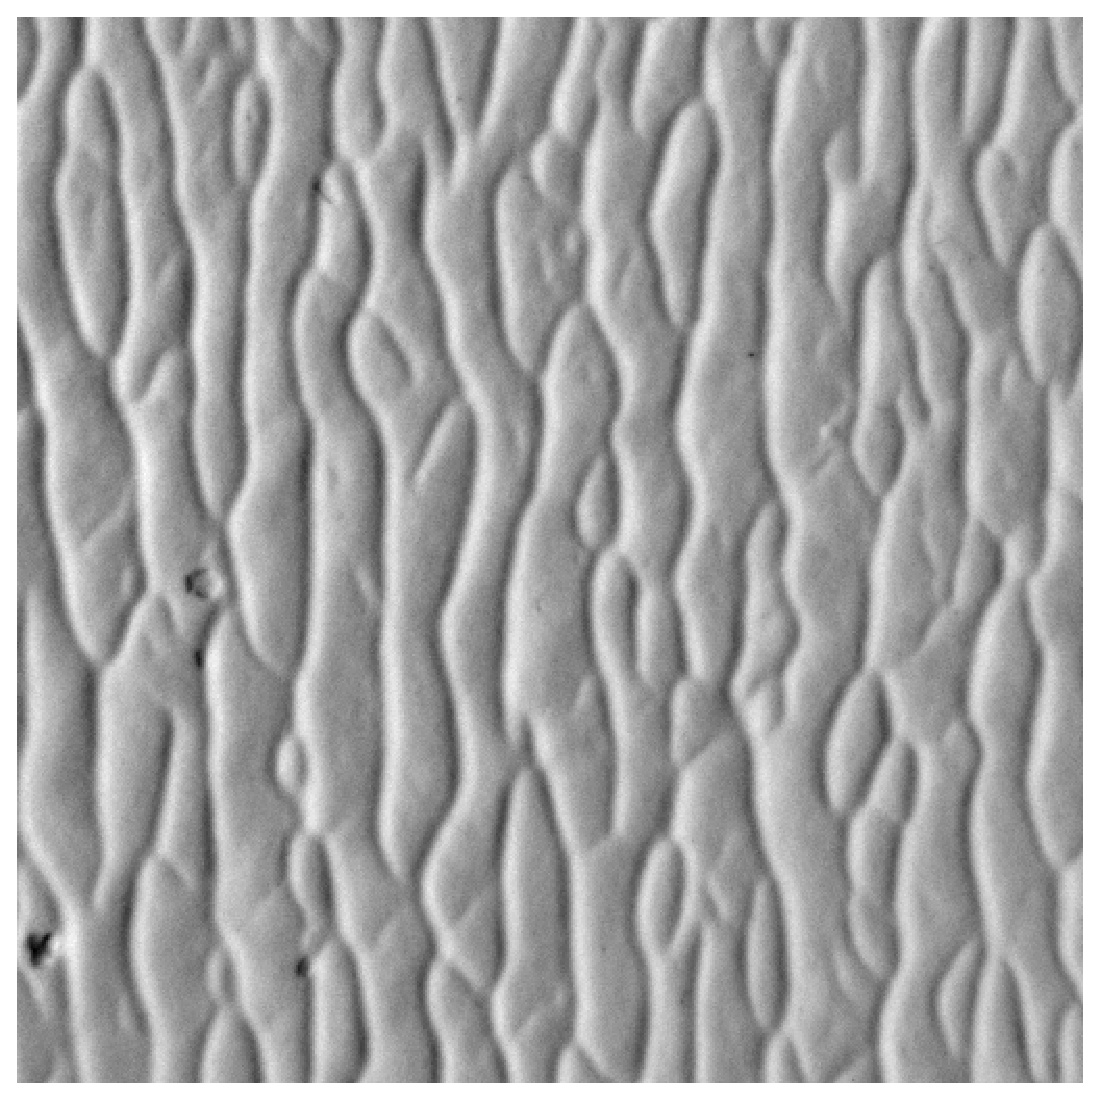
\epsfig{file=images/db/abj.eps, width=0.15\linewidth}}
	\end{center}
	\caption{{\it The material classes taken from the PhoTex database. The example images are registered under a slant of $30^0$ and a tilt of $0^0$.}}
	\label{fig:PhoTexData2}
\end{figure}
%\end{comment}

\section{Reflection model parameters}\label{sec:ParameterSetting}
The reflection models used in the process of synthesis need material dependent parameters to be set, such as the parameter for the specular lobe size or surface roughness. However, these parameters are not available for the materials in the database in case of the micro-facet models, and in case of the empirical models there are no known 'good' values for the parameters to be set. To set these values, the parameters are computed using a gradient descent procedure with a total sum of squares error estimation:

		\begin{eqnarray*}
			Err(A,A') = \sum_{i=1}^n (a_i - a_i')^2
		\end{eqnarray*}
 
Where $A$ is the original image from the {\it PhoTex} database, and $A'$ is the synthesized image that mimics the original image. By calculating the squared per-pixel error from the original image and the synthetic image, and accumulate this error over all pixels we find the error of the synthetic image with respect to the original image. Accumulating this error over a set of synthetic images with its respective set of original images will give an estimation of the total error for a given parameter configuration. By accumulating the error over sets of images instead of using just one image for the parameter estimation, we hope to avoid potential local minima in the gradient descend. Both synthetic and original image are preprocessed to have zero-mean and unit-variance before the error is calculated, since the features will be extracted from such preprocessed images.

Because the number of materials and the number of parameters to be estimated for each reflection model turn out to be large in total and the error for gradient descend needs to be computed over sets of images, a simplified gradient descend is done. Each parameter is estimated using a defined range of possible values. For the microfacet models, the roughness of a material is $m \in \{0.1, 0.3, 0.5, 0.7, 0.9\}$ and the Fresnel coefficient is $R_f \in \{0.01, 0.03, 0.05, 0.07, 0.09\}$. The shininess constant for Phong and Blinn-Phong reflection is from $\alpha \in \{0.001, 0.01, 1.0, 5.0 10.0, 40.0\}$, and the specular reflection coefficient us from $k_s \in \{0.001 0.01 0.1 0.25 0.5 0.75 1.0\}$. 

The surface albedo and surface normals needed for this procedure are derived for each material from images with light directions registered with a slant of $30^0$ and tilts of $\{0^0, 90^0, 180^0, 270^0\}$. The choice for this configuration of angles over the hemisphere is based on the quality of the recovered surface albedo since a non-uniform configuration of tilts gives rise to specularity in the surface albedo. With a uniform choice of angles over the hemisphere, these outliers have minimal influence.

\section{Experimental Setup}\label{sec:Experiments}
In this section, two experiments are described that will be applied on both the diffuse and glossy/shiny dataset. Three different training sets are considered. These training sets are meant to be used for photometric stereo to compute the surface albedo and surface normals. Listed are the training sets for this procedure and are taken from each class separately:

\begin{itemize}
	\item{\textit{T1} - 20 images {\it pseudo-randomly} selected, as proposed by Targhi}
	\item{\textit{T3} - 4 images randomly selected from \textit{T1}, as proposed by Targhi}
	\item{\textit{TT} - the 4 images under a slant of $30^0$ used for finding parameters, as described in section \ref{sec:ParameterSetting}}
\end{itemize}

Similar results to that of Targhi's experiments have been replicated, but exact results are hard to obtain since the quality of the synthetic image data depends strongly on the input images for the photometric stereo. Targhi uses a {\it pseudo-random} selection procedure to obtain the $T1$ set, where pseudo-random is defined as selecting slant and tilt angles to be uniform over the hemisphere. Unfortunately this pseudo-random selection procedure is not explained in further detail, making it hard to obtain the similar training sets.

Pseudo-random in this research is defined as follows: for every slant, a number of tilts is available. There are three configurations of tilts possible such that the hemisphere is covered uniformly when using tilts in increments of $90^0$. To select the 20 images for each class, slants are chosen randomly, and for each slant, a configuration of 4 tilts is chosen randomly, making a total of 20. Note that in the case of a slant of $30^0$, there is only 1 configuration possible. 

\subsection{Experiment A}
In this experiment, we mimic the images from the $T1$ training set to obtain a synthetic training set. This means that for each training set ($T1$, $T3$ and $TT$) we recover the surface albedo and surface normals. With the recovered maps we create synthetic datasets using the slant and tilt angles from the $T1$ dataset for each of the reflection models, creating a total of 20 synthetic images per material class. The training of the material models will be done using these synthetic datasets, and the test images --- images that are not in $T1$ --- are selected from the original {\it PhoTex} dataset.

\subsection{Experiment B}
To further investigate the quality of the synthetic image data, a similar experiment to that of A is conducted, but now instead of mimicking only the images in the $T1$ training set, we replicate all images from the original datasets. We then perform random sub-sampling validation by measuring classification performance of the models derived from synthetic image data and tested against the original dataset. Synthetic training sets are randomly selected from the synthetic data and a test set is randomly selected from the original data. This process of random sub-sampling validation is repeated a 1000 times to average the results. The training set will be increased in the number of images used for constructing the material models until all synthetic images are used for training. 

The idea behind this experiment is as follows: when one would do this experiment using the original {\it PhoTex} image data, perfect classification accuracy is achieved when all images are used for training material models, and 20 images are used for testing. Clearly this is a case overfitting. However, if we would achieve perfect classification accuracy using only synthetic image data, we have found a model that perfectly mimics the original data. 

\section{Results}\label{sec:Results}
\subsection{Diffuse material dataset}
In table \ref{tab:DiffuseResultsA} the results for experiment A are shown. The results are averaged over 5 repetitions of the experiment. As can be seen, the original image data performs really well when training on one half of the dataset and testing on the other half with an average accuracy of \%95.1525. The accuracy for the synthetic data degrades by around 13\% - 16\% for the different training sets. There is a clear gap between the quality of the synthetic image data and the original image data that has not been covered by any of the reflection models. When comparing the reflection models we have to conclude that no significant improvements are made, not even when comparing the more sophisticated reflection models with the Lambertian reflection model. 
 
\begin{table}
	\center
	\begin{tabular}{l|c|c|c|r}
	Method 				&	T1  	&	T3 		&	TT	\\
	\hline
	Original			&	95.1525	&	95.1525 &	95.1525	\\
	Lambertian 			&	81.2212	&	79.7950	&	78.8125	\\
	Phong 				&	81.2440	&	76.7650 &	79.0825	\\
	Blinn-Phong 		& 	82.3030 &	79.9825 &	78.7163	\\
	Torrance-Sparrow 	&	81.9465 &	79.8075 &	81.0487	\\
	Oren-Nayar 			&	82.1475 &	79.8888 &	79.8187	\\
	\end{tabular}
	\caption{{\it Mean accuracy over 5 repetitions for the diffuse material dataset for 20 images in the training set and 20 images in the test set}}
	\label{tab:DiffuseResultsA}
\end{table}

In figure \ref{fig:DiffusePlotB}, we plotted the averaged accuracy when increasing the number of images until all images from the original dataset are mimicked. As with experiment A, experiment B has been repeated 5 times to average results. 

The plots suggest that again little to no improvement is made when comparing reflection models in the case of the $T3$ and $TT$ training sets. The fact no improvements are measured can be explained by how the photometric stereo does not recover the surface albedo and surface normals very well from the $T3$ and the $TT$ datasets. However, for the $T1$ training set we observe that an improvement of ~3\% is measured on top of the Lambertian reflectance for some of the reflectance models. 

Table \ref{tab:DiffuseResultsB} shows the mean and standard deviation for 40 images in the training set and 20 randomly selected images in the test set when using the $T1$ training set for photometric stereo. In the first row, we show performance of the original data to construct the material models and report an almost perfect classification accuracy. This is to be expected since we are overfitting. When using only synthetic image data however, the accuracy drops about 11\% - 14\%. When comparing the reflection models, some improvements with respect to Lambertian reflectance are reported. 

The best performing model is Blinn-Phong with an accuracy of 88.4347\%, followed up by Torrance-Sparrow with 87.8393\% accuracy , both performing better than Phong reflectance. Oren-Nayar for diffuse reflectance also performs better than Lambertian reflectance. The results of the three better performing reflection models have been positively tested on significance level of 5\% using a paired T-test. The results in the table and plots suggest that a more physically based approach can increase the quality of the synthetic images, since the purely empirical based Phong reflectance performs similar or worse than Lambertian reflectance in all experiments. It also suggests that using more images for photometric stereo improves the quality of the surface albedo and surface normals as long as the light sources are distributed uniformly over the hemisphere.

\begin{table}
	\center
	\begin{tabular}{l|c|r}
	Method 				&	T1 - mean 	& T1 - std \\
	\hline
	Original			&	99.4912		& - \\
	Lambertian 			&	85.3313		& 2.386 \\
	Phong 				&	85.6222		& 2.451 \\
	Blinn-Phong 		& 	88.4347 	& 1.839 \\
	Torrance-Sparrow 	&	87.8393 	& 2.036 \\
	Oren-Nayar 			&	87.6650 	& 2.322 \\
	\end{tabular}
	\caption{{\it Mean accuracy and standard deviation over 5 repetitions for the diffuse material dataset for 40 images in the training set and 20 images in the test set}}
	\label{tab:DiffuseResultsB}
\end{table}

\begin{figure}[H]
	\begin{center}
		\subfigure[T1 dataset]{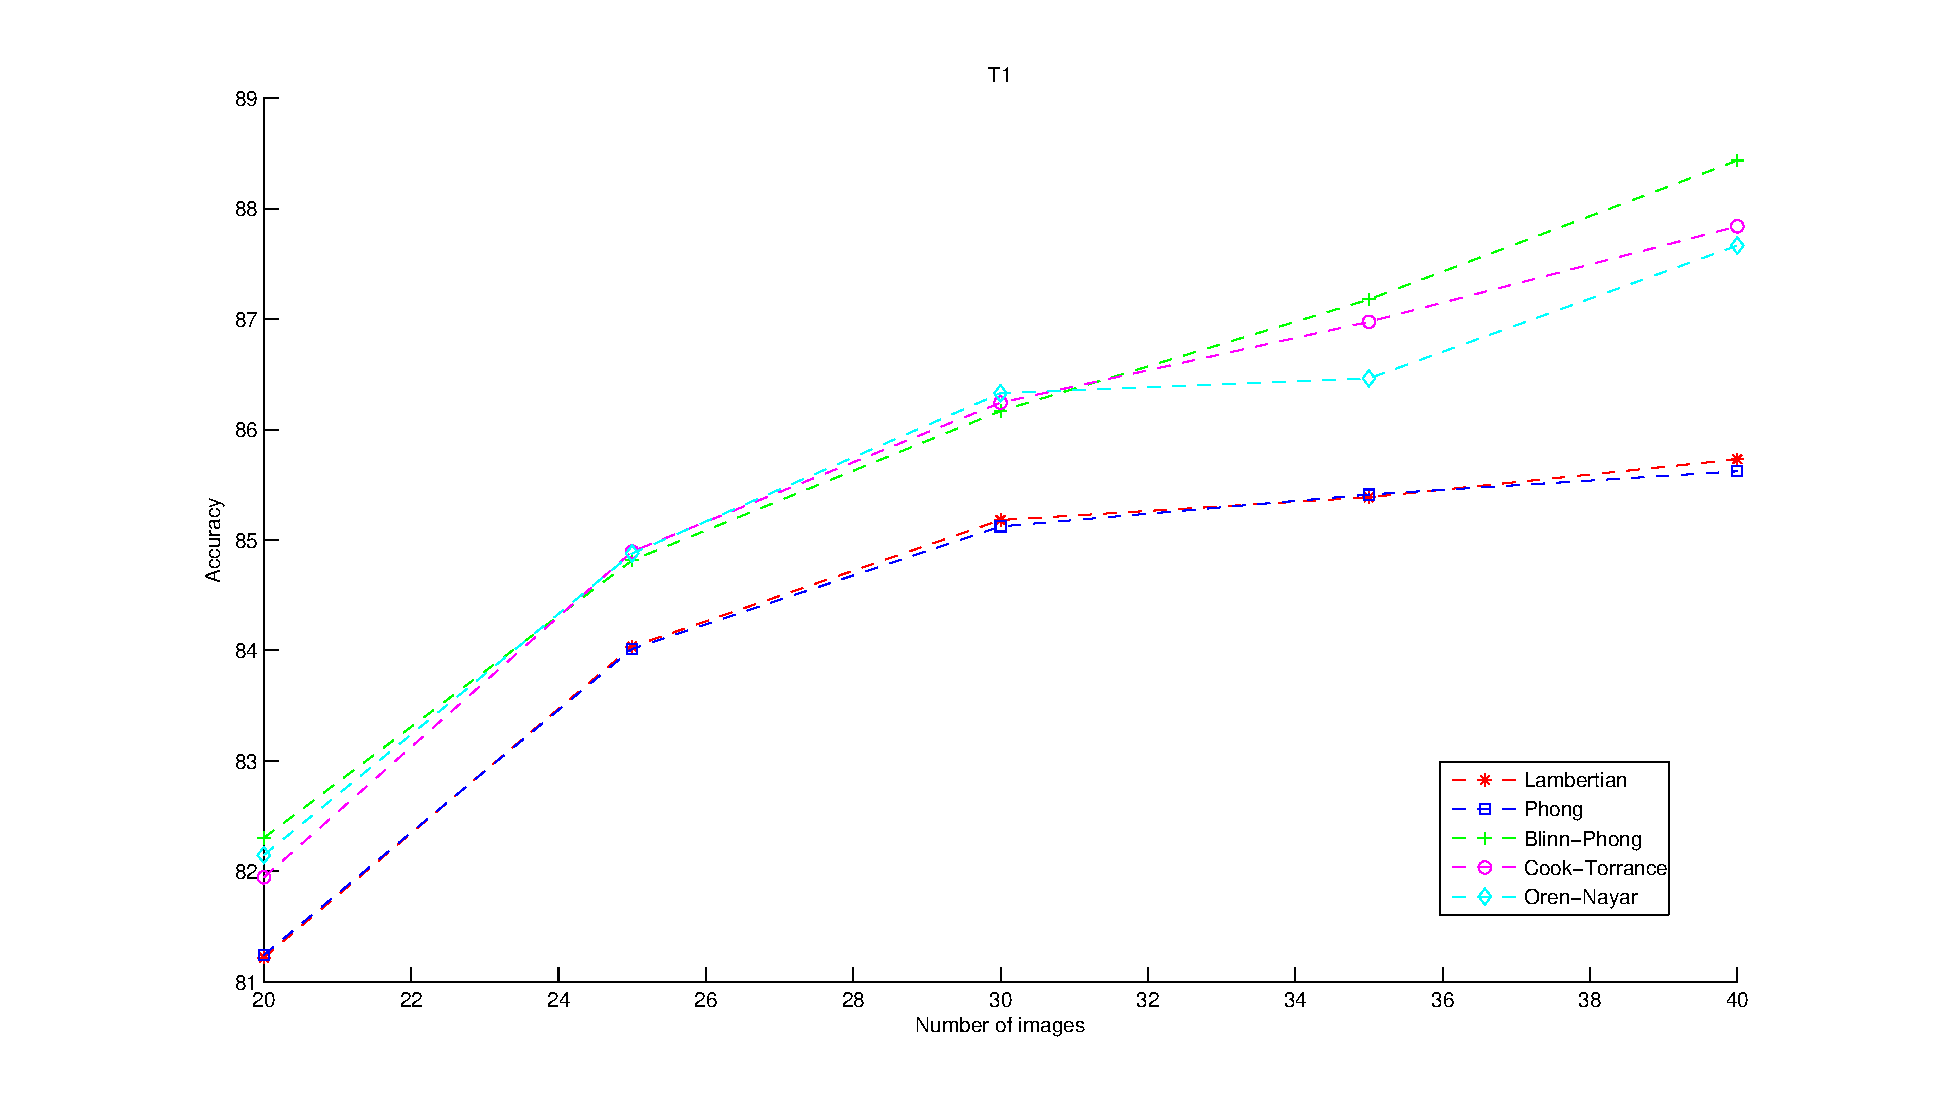
\epsfig{file=images/results/T1.eps, width=0.75\linewidth}}
		\subfigure[T3 dataset]{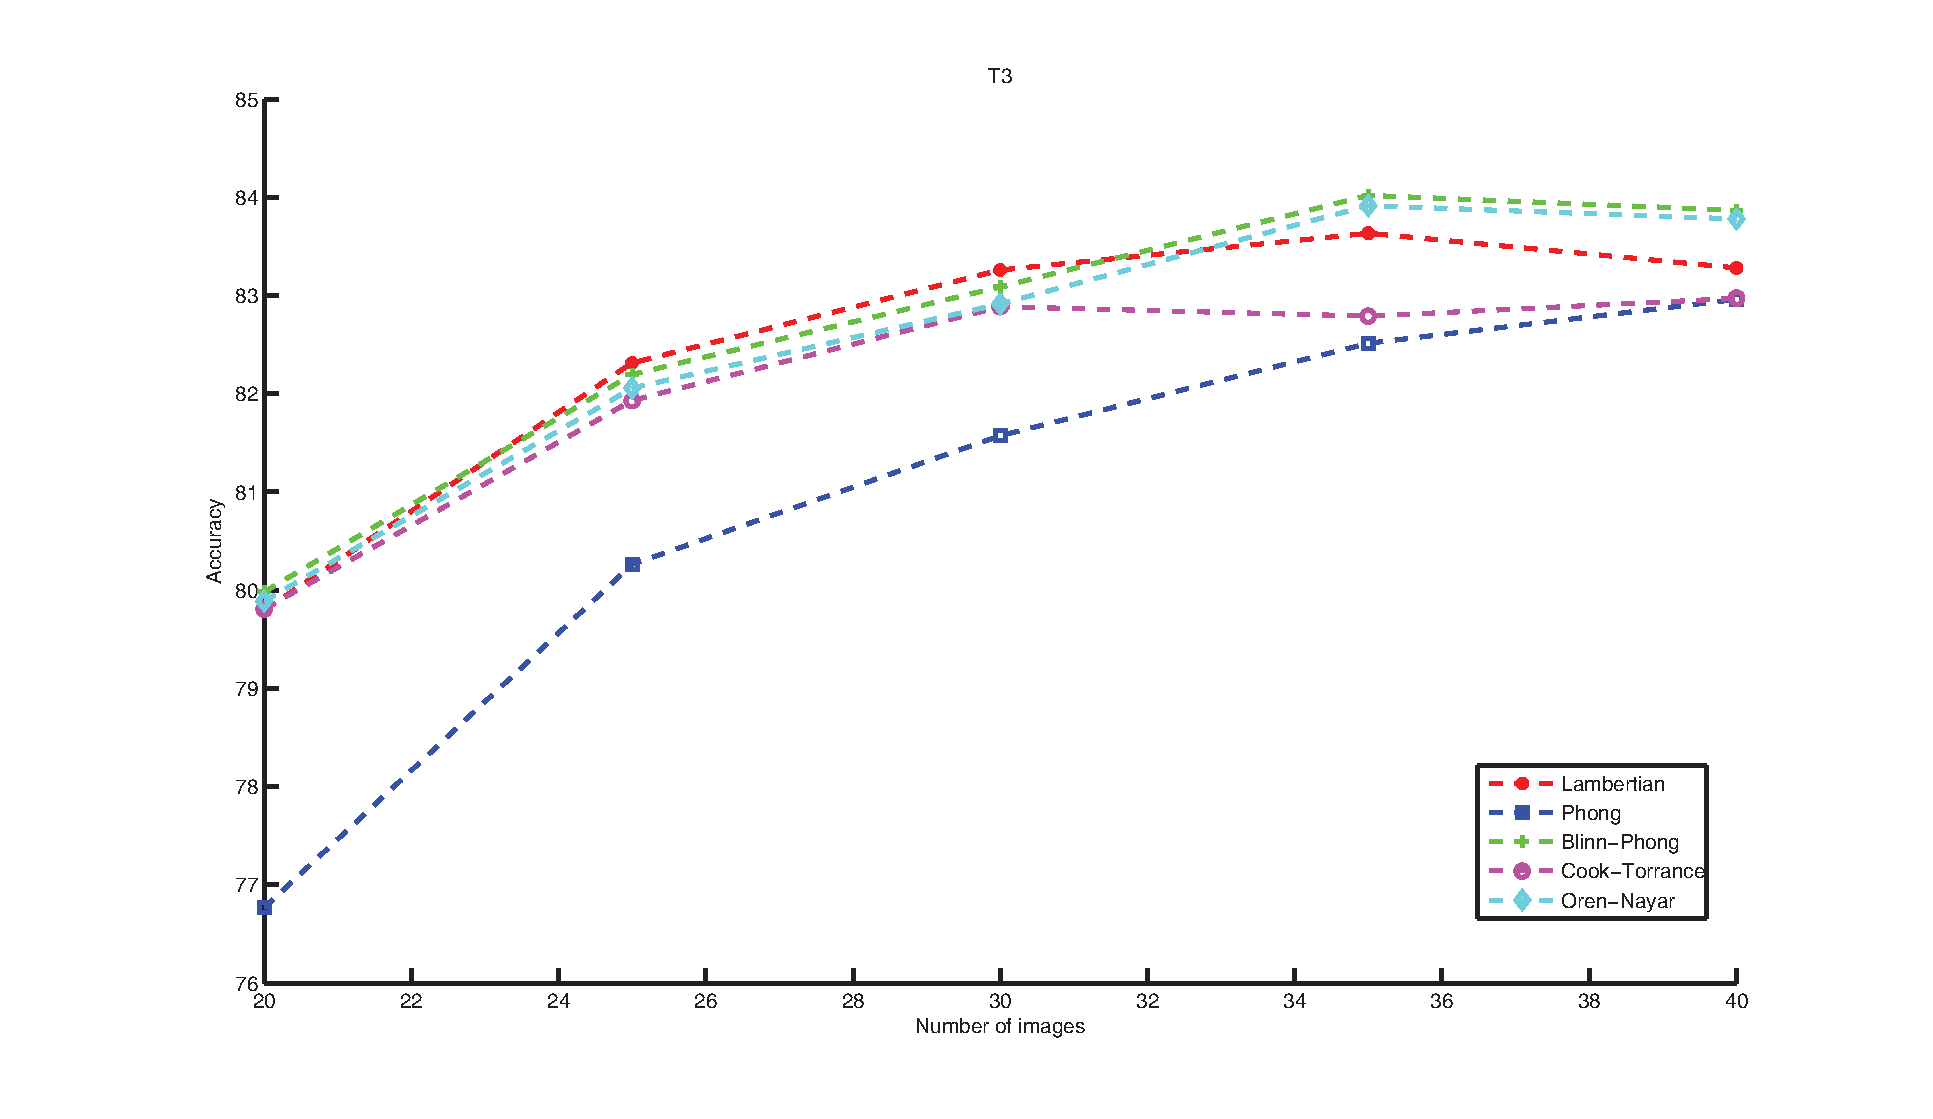
\epsfig{file=images/results/T3.eps, width=0.75\linewidth}}
		\subfigure[TT dataset]{\epsfig{file=images/results/TT.eps, width=0.75\linewidth}}
	\end{center}
	\caption{{\it Results on the T1, T3 and TT dataset for diffuse materials.}}
	\label{fig:DiffusePlotB}
\end{figure}

\subsection{Shiny/glossy material dataset}
For the experiments on the shiny/glossy material dataset we dropped the Phong reflectance for further investigation because of the results found on the diffuse material dataset. We also do not report on results on the $T3$ and $TT$ training sets since these datasets resulted in no significant results in experiment B on the diffuse dataset.

In table \ref{tab:SpecularResultsA} we report the accuracy of the different reflectance models where we have 18 images in the training set and the remaining 18 images in the test set. We observe that the accuracy using synthetic image data has decreased drastically compared to the diffuse material dataset. The difference in accuracy is around 38\% between the original data and the synthetic data. We expect that these results are caused by the poor recovery of the surface albedo and surface normals, since our photometric stereo approach uses a Lambertian surface assumption and the materials in this dataset have a shiny/glossy nature. 

\begin{table}
	\center
	\begin{tabular}{l|c|r}
	Method 				&	T1\\
	\hline
	Original			&	\todo{99.7133}\\
	Lambertian 			&	61.2700\\
	Blinn-Phong 		& 	60.3989\\
	Torrance-Sparrow 	&	61.3722\\
	Oren-Nayar 			&	61.4256\\
	\end{tabular}
	\caption{{\it Mean accuracy and standard deviation over 5 repetitions for the shiny/glossy material dataset for 18 images in the training set and 18 images in the test set}}
	\label{tab:SpecularResultsA}
\end{table}

Running experiment B on this dataset shows similar results even when increasing the amount of images used for the construction of models to the point that all images are used. The material models perform equally bad regardless of the number of images used for photometric stereo or the reflection model used for synthesis as can be observed in figure \ref{fig:SpecularPlotB}. These results stress the importance of having a photometric stereo method with assumptions beyond that of Lambertian surfaces for recovery. Different reflection models cannot improve image quality as they are limited in the recovery from the simple photometric stereo method.

\begin{table}
	\center
	\begin{tabular}{l|c|r}
	Method 				&	T1 - mean 	& T1 - std \\
	\hline
	Original			&	99.7133		& - \\
	Lambertian 			&	60.9289		& 2.5450 \\
	Blinn-Phong 		& 	61.9122 	& 2.6138 \\
	Torrance-Sparrow 	&	61.1278 	& 2.4911 \\
	Oren-Nayar 			&	61.1395 	& 2.6008 \\
	\end{tabular}
	\caption{{\it Mean accuracy and standard deviation over 5 repetitions for the shiny/glossy material dataset for 36 images in the training set and 18 images in the test set}}
	\label{tab:SpecularResultsB}
\end{table}
\begin{figure}[H]
	\begin{center}
		\subfigure[T1 dataset]{\epsfig{file=images/results/T1_specular.eps, width=0.75\linewidth}}
	\end{center}
	\caption{{\it Results on the T1 dataset for specular materials}}
	\label{fig:SpecularPlotB}
\end{figure}




	%___________________________________________________________________________________________
 	\nocite{*}
	\bibliographystyle{plain}
	\bibliography{bibtex}
	\printindex
\end{document}

